%%%%%%%%%%%%%%%%%%%%%%%%%%%%% Define Document %%%%%%%%%%%%%%%%%%%%%%%%%%%%%%%%%%
\documentclass[spanish,12pt,a4paper,twoside,openany]{book}
%%%%%%%%%%%%%%%%%%%%%%%%%%%%%%%%%%%%%%%%%%%%%%%%%%%%%%%%%%%%%%%%%%%%%%%%%%%%%%%
%%%%%%%%%%%%%%%%%%%%%%%%%%%%% Using Packages %%%%%%%%%%%%%%%%%%%%%%%%%%%%%%%%%%
\usepackage[left=1.00in, right=1.00in, top=1.00in, bottom=1.00in]{geometry}
\usepackage{graphicx}
\graphicspath{{img/}}  % Incluir la ruta de la carpeta de imagenes
\usepackage{graphics} %Incluir imagenes pdf
\usepackage{float}
\usepackage{caption}
\usepackage{adjustbox}  % Rotar imagenes
\usepackage{subcaption}  %Ajustar el ancho caption
%INCLUIR PDF
\usepackage{pdfpages}  %incluir pdf
\usepackage{pdflscape} %Rotar una pagina determinada
\usepackage{amssymb}
\usepackage{amsmath}
\usepackage{amsthm}
\usepackage{amsmath}
\setlength{\jot}{1.5ex}
\setlength{\abovedisplayskip}{1.5ex}
\setlength{\belowdisplayskip}{1.5ex}
%%%%%%%%%%%%%%%%%%%%%%%%%%%%%%%%%%%%%%%%%%%%%%%%%%%%%%%%%%%%%%%%%%%%%%%%%%%%%%%%%%
\usepackage{empheq}
\usepackage{mdframed}
\usepackage{booktabs}
\usepackage{longtable} 
\usepackage{lscape}
\usepackage{lipsum}
\usepackage{graphicx}
\usepackage{float}
\usepackage{color}
\usepackage{psfrag}
\usepackage{pgfplots}
\usepackage{bm}
\usepackage{enumitem}
\usepackage[utf8]{inputenc}
\usepackage[spanish,mexico]{babel}
%%%%%%%%%%%%%%%%%%%%%%%%%% Change font %%%%%%%%%%%%%%%%%%%%%%%%%%%%%%%%%%%%%%%%%%
\usepackage[T1]{fontenc}
%\usepackage{helvet}  % Paquete para cambiar la fuente a Helvetica
\renewcommand{\familydefault}{\sfdefault} % Configurar la familia de fuentes como sans serif (Helvetica)
\usepackage{setspace}
%\singlespacing  % Esaciado simple
%\onehalfspacing % Espaciado 1.5
\doublespacing
%%%%%%%%%%%%%%%%%%%%%%%%%%%%%%%%%%%%%%%%%%%%%%%%%%%%%%%%%%%%%%%%%%%%%%%%%%%%%%%%
\usepackage{amssymb}
\usepackage{appendix}
%%%%%%%%%%%%%%%%%%%%%%%%%% Color define %%%%%%%%%%%%%%%%%%%%%%%%%%%%%%%%%%%%%%%
\usepackage{xcolor}
%%%%%%%%%%%%%%%%%%%%%%%%%%%%%%%%%%%%%%%%%%%%%%%%%%%%%%%%%%%%%%%%%%%%%%%%%%%%%%%

%%%%%%%%%%%%%%%%%%%%%%%%%%%% Referencia Bibliográfica %%%%%%%%%%%%%%%%%%%%%%%%%
\usepackage{csquotes}
%\DeclareUnicodeCharacter{0301}{\'{e}} 
\usepackage[style=iso-authoryear]{biblatex}
\addbibresource{bibliography/biblatex-iso690-examples.bib}

%%%%%%%%%%%%%%%%%%%%%%%%%%%%%%%%%%%%%%%%%%%%%%%%%%%%%%%%%%%%%%%%%%%%%%%%%%%%%%
%%%%%%%%%%%%%%%%%%%%%%%%%%%%%% Creative Commnons %%%%%%%%%%%%%%%%%%%%%%%%%%%%%
\usepackage[
type={CC},
modifier={by-nc-nd},
version={4.0},
]{doclicense}

%%%%%%%%%%%%%%%%%%%%%%%%%%%%%%%%%%%%%%%%%%%%%%%%%%%%%%%%%%%%%%%%%%%%%%%%%%%%%%
%%%%%%%%%%%%%%%%%%%%%%%%%%%%% Color links %%%%%%%%%%%%%%%%%%%%%%%%%%%%%%%%%%%%
\usepackage{hyperref}
\hypersetup{
	colorlinks=true,
	citecolor=orange,
	linkcolor=red, %Cambiar al color de preferencia
	filecolor=magenta,      
	urlcolor=cyan,
	pdftitle={Overleaf Example},
	pdfpagemode=FullScreen,
}
\urlstyle{same}
%%%%%%%%%%%%%%%%%%%%%%%%%%%%%%%%%%%%%%%%%%%%%%%%%%%%%%%%%%%%%%%%%%%%%%%%%%%%%%%
%\usepackage{showframe}
%%%%%%%%%%%%%%%%%%%%%%%%%%%%%%%%%%%%%%%%%%%%%%%%%%%%%%%%%%%%%%%%%%%%%%%%%%%%%%
%%%%%%%%%%%%%%%%%%%%%%%%% Chapter Configuration %%%%%%%%%%%%%%%%%%%%%%%%%%%%%%%
\usepackage{titlesec}
\titleformat{\chapter}[block]
{\normalfont\bfseries\Large}{\thechapter.}{0.5em}{\Large}

\titleformat{\section}
{\normalfont\bfseries\large}{\thesection}{0.5em}{\large}

\titleformat{\subsection}
{\normalfont\bfseries\large}{\thesubsection}{0.5em}{\large}

\renewcommand{\thechapter}{\Roman{chapter}}
\renewcommand{\thesection}{\arabic{chapter}.\arabic{section}}
\renewcommand{\thesubsection}{\arabic{chapter}.\arabic{section}.\arabic{subsection}}
\titlespacing*{\chapter}{0pt}{-30pt}{12pt}
\setlength{\parskip}{0mm}

\renewcommand{\thetable}{\arabic{chapter}.\arabic{table}}
\renewcommand{\thefigure}{\arabic{chapter}.\arabic{figure}}

%%%%%%%%%%%%%%%%%%%%%%%%%%%%%%%%%%%%%%%%%%%%%%%%%%%%%%%%%%%%%%%%%%%%%%%%%%%%%%%
%%%%%%%%%%%%%%%%%%%%%%%%%%%%%% Configuration Table of contents %%%%%%%%%%%%%%%%%%
\usepackage{tocloft}
\usepackage{titletoc}

%%%%%%%%%%%%%%%%%%%%%%%%%%%%%%%%%%%%%%%%%%%%%%%%%%%%%%%%%%%%%%%%%%%%%%%%%%%%%%
%%%%%%%%%%%%%%%%%%%%%%%%%% Encabezados %%%%%%%%%%%%%%%%%%%%%%%%%%%%%%%%%%%%%%%
\usepackage{fancyhdr}
\pagestyle{plain}
\fancyhf{}
\fancyhead[LE,RO]{\thepage}
\fancyhead[RE,LO]{\leftmark}
\renewcommand{\headrulewidth}{0.4pt}
%%%%%%%%%%%%%%%%%%%%%%%%%%%%%%%%%%%%%%%%%%%%%%%%%%%%%%%%%%%%%%%%%%%%%%%%%%%%%%
%%%%%%%%%%%%%%%%%%%%%%%%%% Acronym %%%%%%%%%%%%%%%%%%%%%%%%%%%%%%%%%%%%%%%
\usepackage[acronymlists={label-list}]{glossaries}
\newacronym{html}{HTML}{Hypertext Markup Language}
\newacronym{css}{CSS}{Hojas de Estilo en Cascada}
\newacronym{js}{JS}{JavaScript}
\newacronym{pip}{PIP}{Proyectos de inversión pública}
\newacronym{ong}{ONG}{Organismo no gubernamental}
\newacronym{mdt}{MDT}{Municipalidad Distrital de Tamburco}
\newacronym{uep}{UEP}{Unidad de Estudios y Proyectos}
\newacronym{sgodur}{SGODUR}{Sub-Gerencia de Obras Desarrollo Urbano y Rural}
\newacronym{uoem}{UOEM}{Unidad de Obras y Equipos Mecánicos}
\newacronym{uslo}{USLO}{Unidad de Supervisión y Liquidación de Obras}
\newacronym{ucdur}{UCDUR}{Unidad de Catastro Desarrollo Urbano y Rural}
\newacronym{utc}{UTC}{Unidad de Transporte y Circulación}
\newacronym{ioarr}{IOARR}{Inversiones de Optimización, Ampliación Marginal, de Rehabilitación y Reposición}
\makeglossaries
%%%%%%%%%%%%%%%%%%%%%%%%%%%%%%%%%%%%%%%%%%%%%%%%%%%%%%%%%%%%%%%%%%%%%%%%%%%%%%
%%%%%%%%%%%%%%%%%%%%%%%%%%%%%%% Title & Author %%%%%%%%%%%%%%%%%%%%%%%%%%%%%%%%
\title{MANTENIMIENTO DE PISTAS EN LA AV. TAMBURCO-ABANCAY-APURÍMAC}
\author{Juan Benito Quintana Arone}
%%%%%%%%%%%%%%%%%%%%%%%%%%%%%%%%%%%%%%%%%%%%%%%%%%%%%%%%%%%%%%%%%%%%%%%%%%%%%%%
%\usepackage{showframe}

\begin{document}
%\maketitle
\newcommand{\mytitulo}{MANTENIMIENTO DE PISTAS EN LA AV. TAMBURCO-ABANCAY-APURÍMAC}
%%%%%%%%%%%%%%%%%%%%%%%%%%%%%%%%%%%%%%%%%%%%%%%%%%%%%%%%%%%%%%%%%%%%%%%%%%%%%%%
\frontmatter

\begin{titlepage}
	\begin{center}
		\textsf{\textbf{\LARGE UNIVERSIDAD NACIONAL MICAELA BASTIDAS DE APURÍMAC.}}\\
		\vspace{5mm}
		\textsf{\textbf{\Large FACULTAD DE INGENIERÍA}}\\
		\vspace{5mm}
		\textsf{\textbf{ \Large ESCUELA ACADÉMICO PROFESIONAL DE INGENIERÍA CIVIL}}\\
		\vspace{5mm}	
		\begin{figure}[h!]
			\centering
			
\includegraphics[width=0.3\linewidth]{0.2.pdf}
		\end{figure}
		
		\vspace{3mm}	
		\textsf{\textbf{ \Large INFORME DE PRÁCTICAS PRE-PROFESIONALES:}}\\
		\vspace{7mm} {\Large \textbf{''MANTENIMIENTO DE PISTAS EN LA AV. TAMBURCO DEL DISTRITO DE TAMBURCO –PROVINCIA DE ABANCAY – REGIÓN DE APURÍMAC''}}\\
		
		\vspace{5mm}
		\textsf{\textbf{ \Large PRESENTADO POR:}}\\
		\vspace{5mm}
		{\Large\textsf{JUAN BENITO QUINTANA ARONE}}\\
		
		
	
		\vfill
		\textsf{\textbf{ \Large ABANCAY-PERÚ}}\\
		\vspace{5mm}
		\textsf{\textbf{ \LARGE 2023}}\\
		\end{center}
\end{titlepage}



\begin{titlepage}
	\begin{center}
		\textsf{\textbf{\LARGE UNIVERSIDAD NACIONAL MICAELA BASTIDAS DE APURÍMAC.}}\\
		\vspace{4mm}
		\textsf{\textbf{\Large FACULTAD DE INGENIERÍA}}\\
		\vspace{4mm}
		\textsf{\textbf{ \large ESCUELA ACADÉMICO PROFESIONAL DE INGENIERÍA CIVIL}}\\
		\vspace{4mm}	
		\begin{figure}[h!]
			\centering
			
\includegraphics[width=0.25\linewidth]{0.1.pdf}
		\end{figure}
		
		\vspace{3mm}	
		\textsf{\textbf{ \Large INFORME DE PRÁCTICAS PRE-PROFESIONALES:}}\\
		\vspace{3mm}
		{\large\textsf{''MANTENIMIENTO DE PISTAS EN LA AV. TAMBURCO DEL DISTRITO DE TAMBURCO – PROVINCIA DE ABANCAY – REGIÓN DE APURÍMAC''}}\\
		\vspace{5mm}
		{\Large\textsf{PRESENTADO POR\\}}
		\textsf{\textbf{ \Large JUAN BENITO QUINTANA ARONE \\}}
		
		\vspace{5mm}	
		{\large \textsf{Sustentado y aprobado el \today, ante el jurado:}}\\
		\vspace{5mm}		

		\begin{flushleft}
			\textsf{\textbf{ \large Presidente	:}}\hspace{18mm} \rule{10cm}{0.4pt}\\
			%\hspace{3cm} %\textnormal{\sffamily Ph.D: Lucy M. Guanuchi Orellana} \\
			\vspace{10mm}
			\textsf{\textbf{ \large Primer miembro	:}}\hspace{5mm} \rule{10cm}{0.4pt}\\
			%\hspace{3cm} \textnormal{\sffamily Dr: Nelson Palemon Meza Peña} \\		
			\vspace{10mm}
			\textsf{\textbf{ \large Segundo miembro	:}} \rule{10cm}{0.4pt}\\
			%\hspace{3cm} \textnormal{\sffamily Mstro: Feliciano Escobedo Silva} \\		
			%\vspace{3mm}
			%\textsf{\textbf{ \large Asesor	:}} \rule{8cm}{0.4pt}\\	
			%\hspace{3cm} \textnormal{\sffamily Mgt: Calixto Cañari Otero} \\	
		\end{flushleft}
		
		\vfill
		
	\end{center}
\end{titlepage}


\newpage
\pagestyle{plain}
%\vspace*{20cm}
\vspace*{\fill}
 
\doclicenseThis ,El presente proyecto, pertenece a la linea de investigación denominado
El autor autoriza a la Universidad Nacional Micaela Bastidas de Apurímac a reproducir la tesis en su totalidad o en parte, con fines estrictamente académicos.
En particular esta licencia no permite venta ni modificaciones de este material.
	




\newpage
\pagestyle{plain}
\vspace*{\fill} %Centrar verticalmente en la pagina
\begin{flushright}%Alinea a la izquierda
	\begin{minipage}[t]{0.6\textwidth}
		{\LARGE\textbf{Dedicatoria}\\}
		
	En este día tan especial, quiero dedicarles mi tesis a mis padres Teresa, Benito y mis hermanos como una muestra de gratitud y reconocimiento a cada uno de ustedes. Su presencia en mi vida ha sido un regalo inmenso y estoy infinitamente agradecido por tenerlos a mi lado.
		
	\end{minipage}
\end{flushright}

\vspace*{\fill}
\newpage
\pagestyle{plain}
\vspace*{\fill} %Centrar verticalmente en la pagina
\begin{flushleft}%Alinea a la izquierda
	\begin{minipage}[t]{0.7\textwidth}
		{\LARGE\textbf{Agradecimientos}\\}
		En primer lugar, quiero agradecer a Dios por su amor y guía constante en mi vida. Ha sido mi fuerza y mi refugio en los momentos de desafío. Su bendición ha sido fundamental en cada paso del camino.
		
		A mis padres Teresa y Benito, quiero expresarles mi profundo agradecimiento por su amor inquebrantable y su apoyo incondicional. Han sido mis pilares, siempre presentes para brindarme palabras de aliento, ánimo y sabiduría en cada etapa de mi vida universitaria. 
		
		A mis hermanos, gracias por ser mis compañeros de vida y mis mayores motivadores. Su apoyo incondicional y su fe en mí me han impulsado a seguir adelante incluso en los momentos más desafiantes. 
		
		\vspace{5mm}
		
		Con profundo amor y gratitud,\\
		\vspace{5mm}
		Juan Benito Quintana Arone
		
		
		
	\end{minipage}
\end{flushleft}

\vspace*{\fill}
\newpage
\tableofcontents
\newpage
\listoftables
\newpage
\listoffigures
\newpage
\printglossary[type=\acronymtype, title={Siglas y Acrónimos}]
%%%%%%%%%%%%%%%%%%%%%%%%%%%%%%%%%%%%%%%%%%%%%%%%%%%%%%%%%%%%%%%%%%%%%%%%%%%%%%%%
\mainmatter
\chapter*{RESUMEN}

En resumen 


\lipsum[5] 
\pagestyle{myheadings}
\chapter{DATOS GENERALES DEL ALUMNO}
		\noindent \textbf{Apellidos y nombres:} Quintana Arone Juan Benito \\
		\textbf{Código}:152254\\
		\textbf{Último ciclo de estudios terminado:}2023-I\\
		\textbf{Créditos aprobados:203 créditos }\\
		\textbf{Docente asesor:}Ph.:Lucy Marisol Guanuchi Orellana\\
%\pagestyle{fancy}
\chapter{DATOS GENERALES DE LA ENTIDAD}
\section{Nombre:}
Municipalidad Distrital de Tamburco\\

\begin{figure}[h!]
	\captionsetup{width=0.4\textwidth}
	\centering
	
\includegraphics[width=0.4\linewidth]{2.2.pdf}
	\caption[Logotipo de la Municipalidad Distrital de Tamburco]{Logotipo de la Municipalidad Distrital de Tamburco}
	\label{fig:mdt-1}
\end{figure}

\section{Razón social:}
\noindent Municipalidad Distrital de Tamburco\\
R.U.C:20175824619

\section{Actividad específica:}
\noindent Principal - 8411 - Actividades de la administración pública en general.\\
La Municipalidad Distrital de Tamburco es una entidad pública, como se muestra en la figura \ref{fig:organigrama-tamburco}, se subdividen en 5 sub-gerencias:sub-gerencia de administración y finanzas, sub-gerencia de adminsitración tributaria y rentas, sub-gerencia de desarrollo económico, social y cultural, sub-gerencia dee obras y desarrollo urbano y rural y sub-gerencia de recursos naturales y gestión ambiental.
\section{Dirección:}
\noindent Dirección legal:Plaza. De armas S/N Cercado (a lado del parque).\\
Departamento:Apurímac\\
Provincia:Abancay\\
Distrito:Tamburco
\begin{figure}[h!]
	\captionsetup{width=0.8\textwidth}
	\centering
	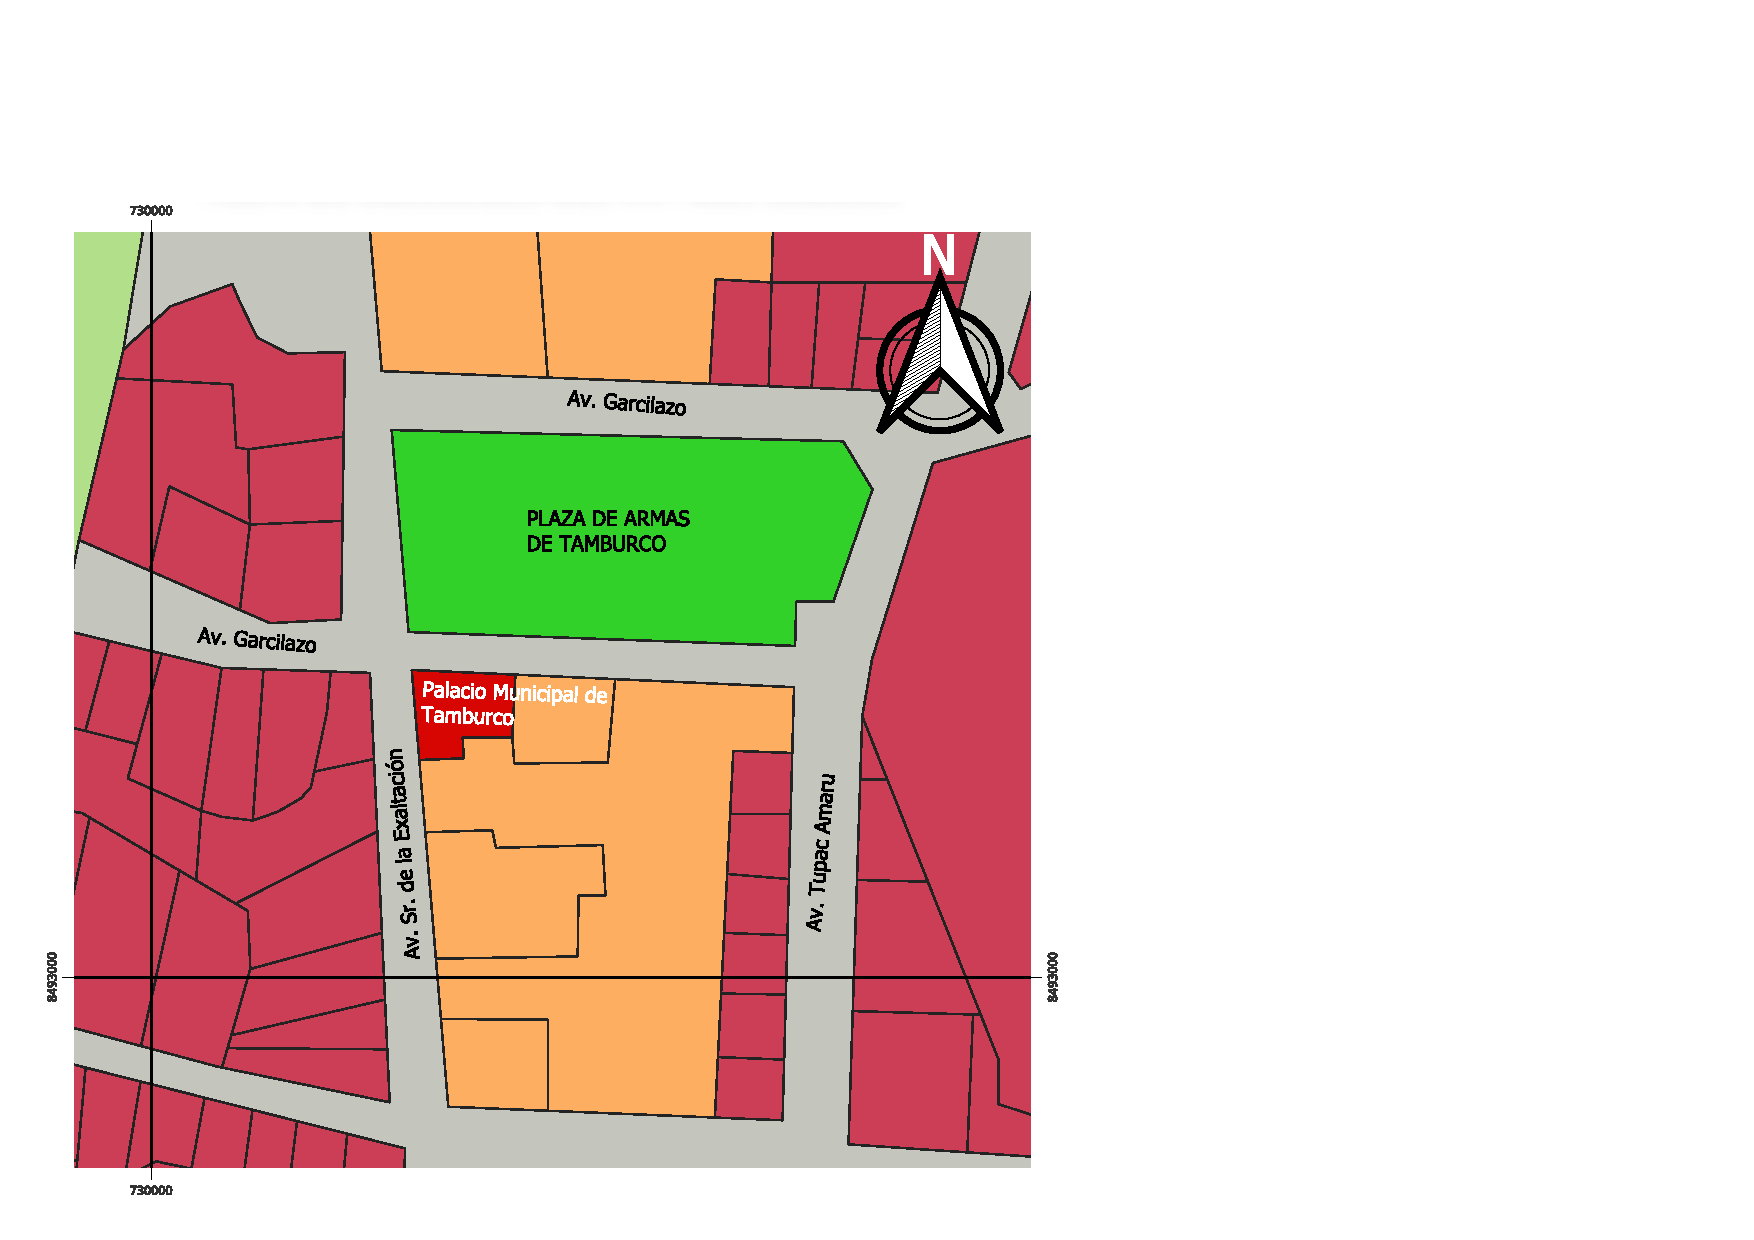
\includegraphics[width=0.8\textwidth]{2.0.pdf}\\
	\caption[Mapa de ubicación del Palacio Municipal]{Ubicación de la Municipalidad Distrital de Tamburco}
	\label{map_ubic}
\end{figure}
\section{Nombre del Representante Legal:}
\noindent Raúl Silva Campos\\
\textbf{Alcalde de la Municipalidad Distrital de Tamburco}

\section{Nombre del Jefe Inmediato:}
\noindent Ing. Ricardo Hemrich Pinto Yupanqui, Sub Gerente de Obras y Desarrollo Urbano y Rural.\\

\section{Teléfonos:}
\begin{itemize}
	\item Jefe Inmediato: 952717755
	\item Representante Legal:
\end{itemize}

\vspace{3mm}
\begin{figure}[h!]
	\captionsetup{width=0.8\textwidth}
	\centering
	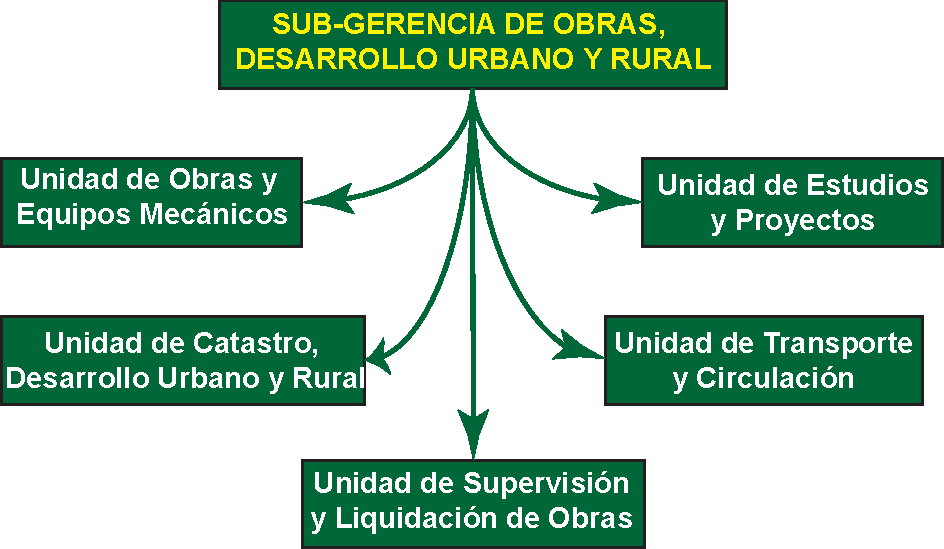
\includegraphics[width=0.8\textwidth]{2.5.pdf}
	\caption{Distribución en unidades de la SGODUR}
	\label{fig:2.5}
\end{figure}
\newpage
\begin{figure}[H]
	\centering
	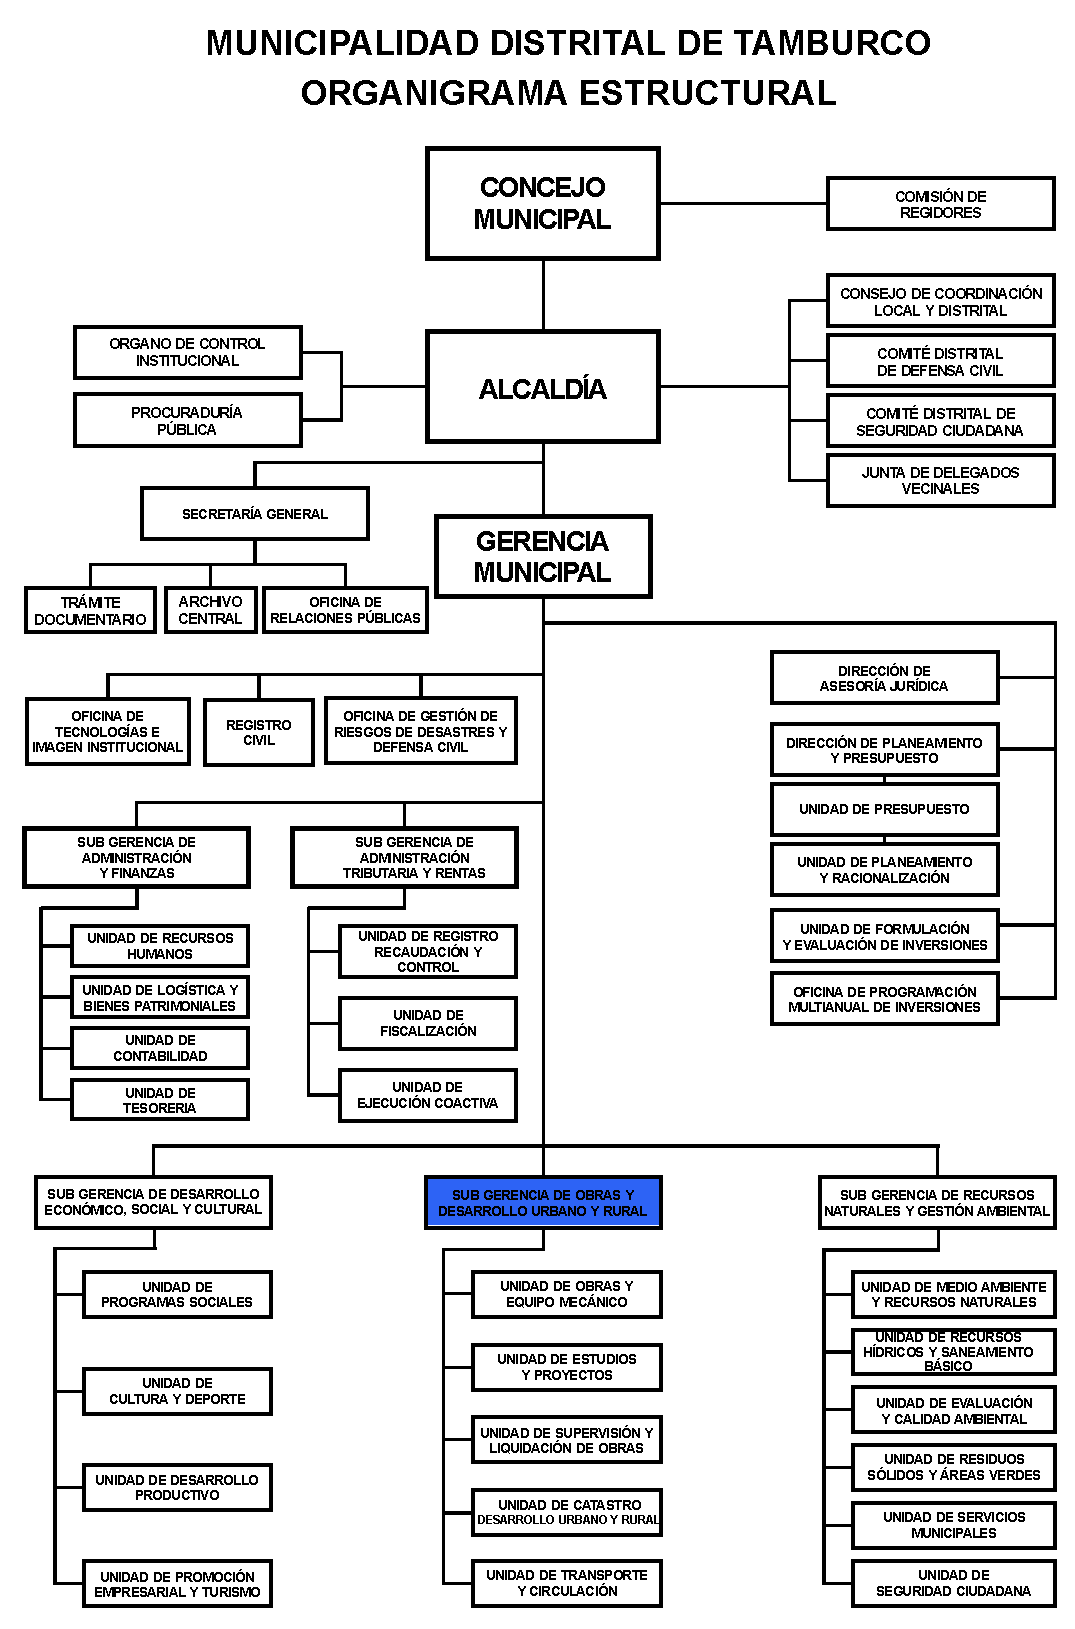
\includegraphics[height=24cm]{2.4.pdf}
	\caption[Organigrama de la Municipalidad Distrital de Tamburco]{Fuente:Municipalidad Distrital de Tamburco}
	\label{fig:organigrama-tamburco}
\end{figure}
%\pagestyle{fancy}
\chapter{PROCESOS DESARROLLADOS DURANTE LA PRÁCTICA}\label{procesos-desarrollados}
\section{Objetivos}
\subsection{Objetivos generales}
\begin{itemize}
	\item Afianzar los conocimientos teóricos adquiridos en las sesiones académicas durante la formación universitaria es esencial para la preparación integral de un futuro profesional. Las prácticas pre-profesionales en la Sub Gerencia de Obras y Desarrollo Urbano y Rural, específicamente en el área de Unidad de Obras y Equipo Mecánico, proporcionan una oportunidad valiosa para aplicar y consolidar esos conocimientos en un entorno laboral real. Esta experiencia práctica no solo brinda una comprensión más profunda de los conceptos teóricos, sino que también permite desarrollar habilidades específicas y aprender cómo se aplican en situaciones concretas. Este enfoque integrado entre teoría y práctica contribuye significativamente al crecimiento y desarrollo profesional del estudiante.

\end{itemize}
\subsection{Objetivos específicos}
\begin{itemize}
	\item Ampliar los conocimientos sobre la gestión pública, en concordancia con las directrices y normativas establecidas por la Municipalidad Distrital de Tamburco, es una prioridad para cualquier profesional que aspire a contribuir de manera efectiva en el ámbito público. Estar al tanto de las regulaciones y lineamientos específicos de la entidad local no solo facilita la toma de decisiones informadas, sino que también asegura que las acciones y proyectos estén alineados con los objetivos y metas de la municipalidad. Esto fortalece la capacidad del profesional para desempeñarse con eficiencia y eficacia en el entorno de la gestión pública, maximizando el impacto positivo de sus contribuciones.
	\item Adquirir conocimientos en la elaboración de fichas técnicas con fondos asignados por el Ministerio de Economía y Finanzas es una habilidad valiosa para cualquier profesional involucrado en proyectos financiados por entidades gubernamentales. Estas fichas técnicas son documentos detallados que describen de manera precisa y completa los aspectos técnicos y financieros de un proyecto, proporcionando la información necesaria para su planificación y ejecución efectiva. Dominar esta habilidad asegura que los proyectos se formulen y presenten de manera adecuada, cumpliendo con los requisitos y estándares establecidos por el Ministerio de Economía y Finanzas. Esto, a su vez, contribuye al éxito y viabilidad de los proyectos financiados por esta entidad.
	\item Ampliar y profundizar el dominio de software esencial en el campo de la ingeniería es una excelente manera de fortalecer tus habilidades profesionales. Esto incluye herramientas como AutoCAD 2021, Revit, AutoCAD Civil 3D, QGIS y Excel 2021, que son cruciales para el diseño, modelado y análisis en ingeniería civil. Asimismo, familiarizarte con Oracle Primavera P6 te brindará habilidades avanzadas en gestión de proyectos. En cuanto al análisis estructural, programas como ETABS y SAFE son fundamentales y dominarlos te permitirá realizar evaluaciones estructurales detalladas y precisas. Esta inversión en formación y habilidades técnicas te posicionará como un profesional altamente competente en el campo de la ingeniería civil.
	\item La asimilación de experiencia durante la inspección de obras realizadas por administración directa es una oportunidad invaluable para cualquier profesional en el campo de la ingeniería. Durante este proceso, se tiene la oportunidad de observar y participar en la ejecución de proyectos de manera directa, lo que proporciona una comprensión profunda de los aspectos prácticos y operativos de la construcción. Además, permite identificar desafíos comunes y aprender estrategias efectivas para resolver problemas en el sitio de trabajo. Esta experiencia en inspección de obras contribuye significativamente al crecimiento profesional, al enriquecer el conocimiento teórico con la aplicación práctica en el campo de la ingeniería civil.
	\item La capacidad de asimilar conocimientos, experiencias y sugerencias, así como interactuar con diversos profesionales en el entorno laboral, es esencial para el crecimiento y desarrollo como ingeniero civil. Esta interacción enriquecedora brinda la oportunidad de aprender de la experiencia de otros, adquirir nuevas perspectivas y fortalecer habilidades técnicas y profesionales. La diversidad de profesionales con los que se interactúa puede ofrecer valiosos insights y enfoques distintos para abordar desafíos y resolver problemas. Este proceso de aprendizaje continuo y colaborativo contribuye significativamente a la calidad y capacidad como ingeniero civil, permitiendo una evolución constante en el campo de la ingeniería.
\end{itemize}

\section{Descripción del proyecto}
\subsection{Nombre del proyecto}
'' Mantenimiento de pistas en la Avenida Tamburco del Distrito de Tamburco, Abancay - Apurímac ''
\subsection{Estado situacional de la infraestructura}
La infraestructura vial en mención, está como clasificada como vía nacional  PE 30S, las carreteras en el Perú se clasifican de acuerdo a 2 criterios: En función a su demanda y en función a su orografía según menciona \cite[12]{MTC2018}, une las ciudades de Abancay y Cusco, constituido de pavimento flexible que a medida transcurre por zonas urbanas existen intersecciones con pavimentos rígidos.

Cabe aclarar que la vía se encuentra bajo la juridicción de PROVIAS NACIONAL encargado de la ejecución de proyectos de construcción, mejoramiento, rehabilitación y mantenimiento de la Red Vial Nacional, que a su vez concesiona para el mantenimiento a diferentes empresas privadas, en este caso particular es SURVIAL la empresa encargada de tal fin.
En el presente análisis situacional se evidenció deterioro de los siguientes tramos mostrados a continuación:
\begin{enumerate}[noitemsep]
	\item Intersección Av. Tupac Amaru - Av. Tamburco(KM: 775+44-775+74)
	\item Intersección Av. Tamburco-Jr. Señor de Exaltacion (KM: 774+67-775+03)
	\item Intersección Av. Tamburco -Coronel Gonzales(KM: 794+25-795+57)
	\item Intersección Av.Tamburco - 14 de Septiembre(KM: 773+44-773+76.649)
	\item Av. Tamburco (KM: 776+51-776+65)
	\item Intersección Av. Tamburco-Calle Martinelli (KM: 766+51-766+64.14)
	\item Intersección Av. Tamburco- Prolon. Huancavelica(KM: 765+31-765+45.96)
	\item Intersección Av. Tamburco-Prolong. Nuñez(KM: 763+31-763+52.5870)
	\item Av. Tamburco (Grifo REPSOL) (KM: 762+43-763+00)
	\item Intersección Av. Tamburco-Av. Taracalle(KM:761+49.79-761+70.333)
\end{enumerate}

Los tramos mencionados se encuentran actualmente deteriorado ya que el asfalto sufrió un deterioro por el constante tránsito de vehículos de servicio urbano, así como los vehículos de carga pesada que transitan, al ser este una vía nacional clasificada como PE 30S, esta situación hace que se genere una congestión vehicular de manera constante, generando un retraso en el tránsito por la presencia de hoyos, que dificulta el tránsito vehicular.

Debido a la juridicción la Municipalidad Distrital de Tamburco no podría intervenir con ningún proyecto de inversión, por esto la única alternativa viable para dar solución es un convenio inter-institucional suscrito entre PROVIAS-MDT.

Respecto a las causas del desgaste y deterioro existen muchas variables en cuestión, mientras no existan estudios que determinen las causas exactas son opiniones meramente especulativos, como: tiempo de servicio culminado, mala conservación de la infraestructura, uso inadecuado, etc.
\section{Objetivos generales}
Todo proyecto que tenga total o parcialmente financiado por recursos de origen público son administrados según la norma decretada por el \cite{CongresoRepublica2022} con un objetivo claro y bien establecido, siendo los siguientes.

\begin{enumerate}
	\item Mejorar el servicio de transporte y movilidad urbana no solo facilita la accesibilidad y comodidad de los ciudadanos, sino que también puede tener un impacto positivo en la calidad de vida, la economía local y el medio ambiente. Para lograrlo, es importante considerar estrategias que incluyan el diseño eficiente de rutas y medios de transporte, la implementación de tecnologías y sistemas de gestión, así como la promoción de opciones de movilidad sostenible. Además, es fundamental contar con la participación y retroalimentación activa de la comunidad para asegurar que las soluciones propuestas sean adecuadas y efectivas.
	\item Para mejorar el servicio de transporte y la movilidad urbana, es fundamental proporcionar una experiencia de conducción más cómoda y suave para los usuarios. Esto implica no solo mantener en óptimas condiciones la infraestructura vial, reparando baches y nivelando calles, sino también implementar una señalización clara y eficaz que permita a los conductores anticipar las condiciones de la vía. Asimismo, se debe planificar rutas eficientes que minimicen el tráfico y se deben invertir en mejoras en el transporte público, fomentando su uso como una alternativa viable al vehículo privado. Promover la movilidad sostenible, utilizar tecnologías avanzadas de transporte y considerar la comodidad del usuario en paradas y estaciones son pasos esenciales. Además, la educación vial y la concientización sobre prácticas seguras en la vía contribuyen de manera significativa a una experiencia de conducción más fluida y placentera para todos los usuarios.
	\item La implementación de medidas para proporcionar una experiencia de conducción más suave y cómoda no solo beneficia a los usuarios, sino que también conlleva una reducción significativa en los costos de mantenimiento de los vehículos. Al disminuir el desgaste y la necesidad de reparaciones ocasionadas por condiciones adversas en las vías, se logra un ahorro considerable en los recursos destinados a la mantención de la flota automotriz. Esta optimización en los gastos operativos no solo impacta positivamente en el presupuesto, sino que también contribuye a una gestión más eficiente y sostenible de la movilidad urbana.
	\item Sin lugar a dudas, mejorar el estado de las vías urbanas tiene un impacto significativo en la imagen de la ciudad. Una pista en buen estado no solo facilita la movilidad, sino que también transmite una impresión positiva a residentes y visitantes. Calles bien mantenidas sugieren una ciudad cuidada y organizada, lo cual puede fomentar un sentido de orgullo cívico entre la comunidad. Además, una buena infraestructura vial puede atraer inversiones y contribuir al desarrollo económico local. Por lo tanto, invertir en el estado de las vías urbanas no solo mejora la movilidad, sino que también tiene efectos positivos en la percepción y prosperidad de la ciudad en su conjunto.
	\item Una infraestructura vial bien mantenida y planificada no solo mejora la imagen de la ciudad, sino que también tiene un impacto directo en la eficiencia del tráfico. Al proporcionar una superficie de conducción suave y sin obstáculos, se facilita el flujo vehicular y se reduce la congestión. Esto se traduce en tiempos de viaje más cortos y una mayor eficiencia en el desplazamiento de personas y bienes. Además, al disminuir la congestión, se reducen los niveles de contaminación y se mejora la calidad del aire en la ciudad. En resumen, una infraestructura vial en buen estado contribuye de manera significativa a una movilidad más eficiente y sostenible en el entorno urbano.
	\item Una infraestructura vial en óptimas condiciones no solo mejora la movilidad, sino que también juega un papel crucial en la seguridad de conductores y peatones. Al eliminar riesgos como baches y obstáculos en la vía, se reduce significativamente la posibilidad de colisiones y lesiones. Esto crea un entorno más seguro para todos los usuarios de la vía y promueve una convivencia armoniosa entre peatones y conductores. Además, al reducir los riesgos en la vía, se fomenta una cultura vial responsable y se contribuye a la disminución de accidentes, lo que es fundamental para la seguridad y bienestar de la comunidad en general.
\end{enumerate}


\section{Ubicación geográfica}
La ejecución de la presente actividad de mantenimiento integral, del local municipal se encuentra en:
\vspace{3mm}

\begin{tabular}{ll}
	Departamento: & Apurímac \\
	Provincia     & Abancay  \\
	Distrito      & Tamburco
\end{tabular}

\begin{figure}[h]
	\captionsetup{width=0.8\textwidth}
	\centering
	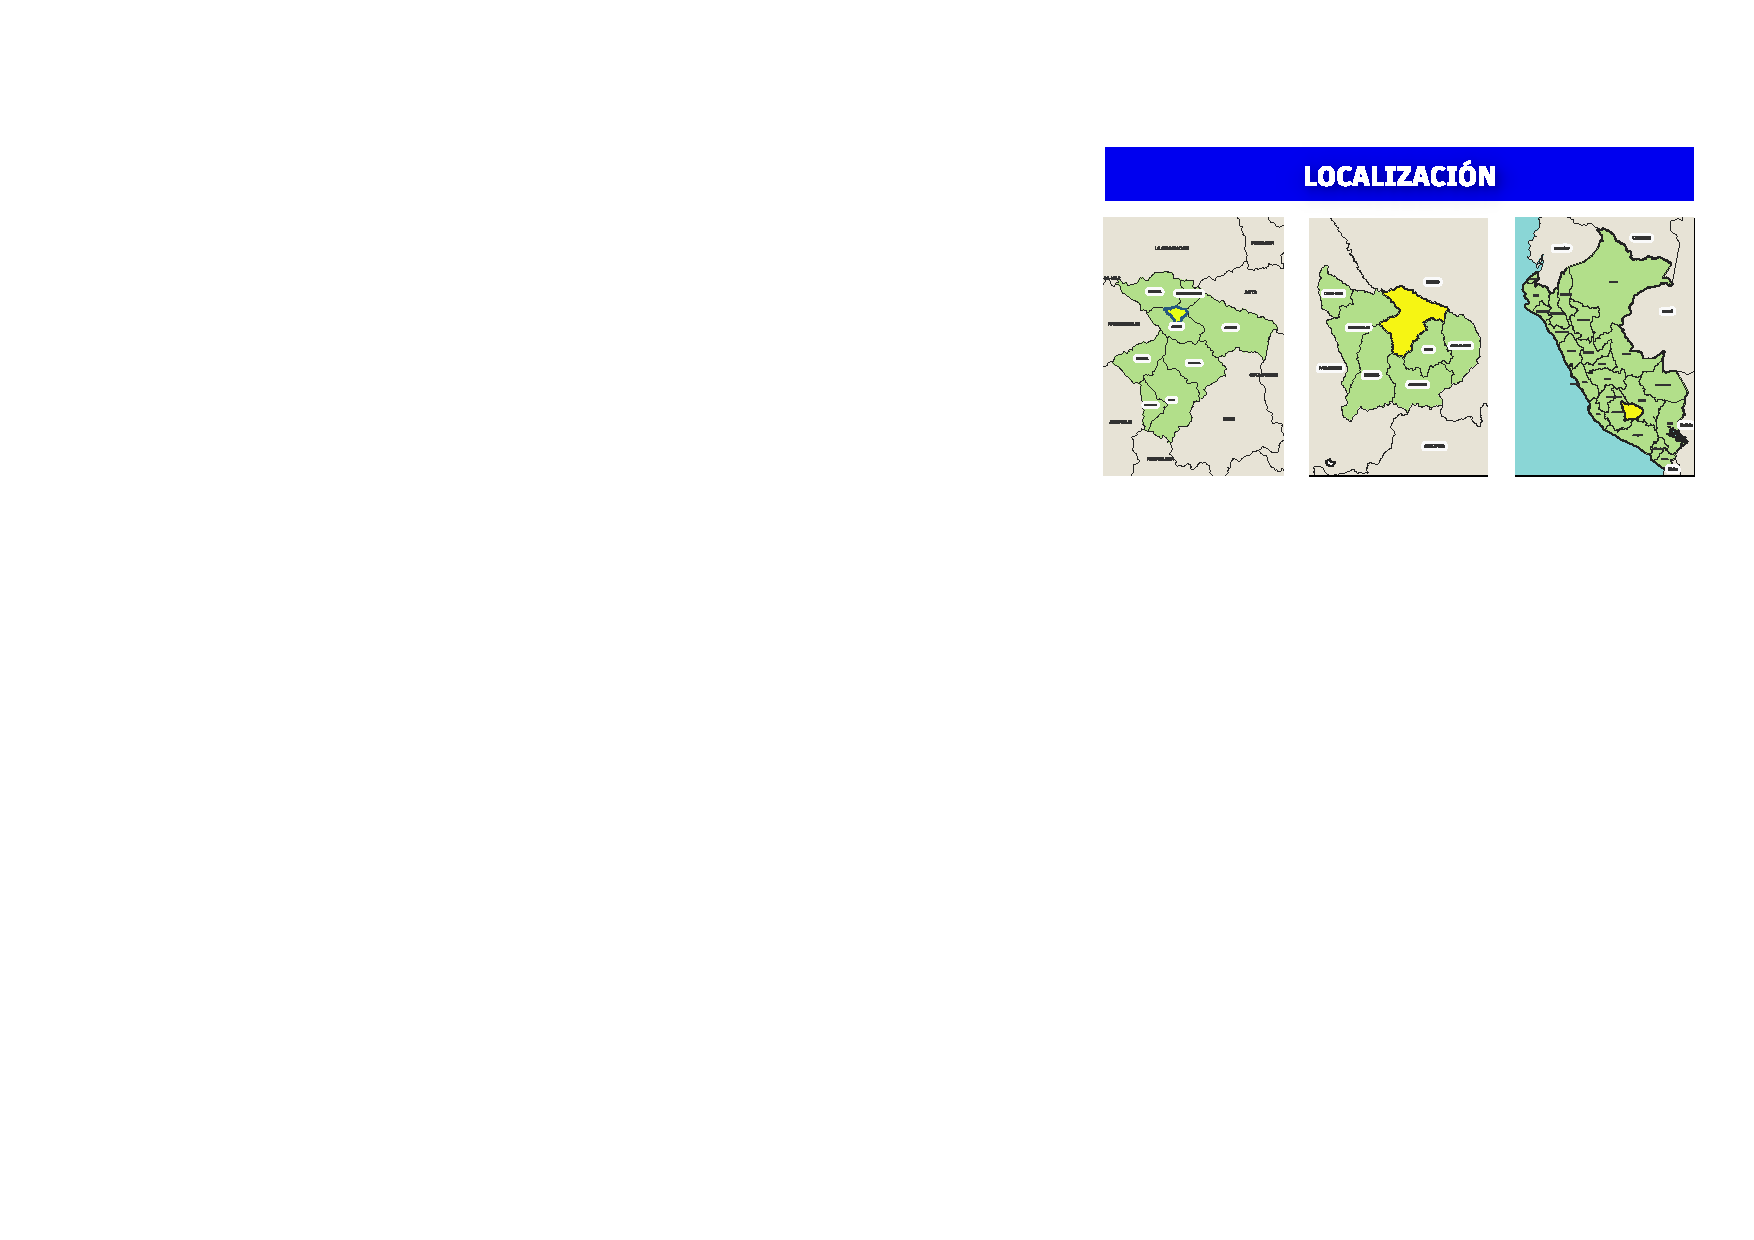
\includegraphics[width=0.8\linewidth]{2.3.pdf}
	\caption[Ubicación geográfica del proyecto]{Los tramos a intervenir están localizados desde la colindancia con el distrito de Abancay, avanza progresivamente hacia el Mirador }
	\label{fig:localizacion}
\end{figure}

\section{Justificación del proyecto}
El presente Plan de Mantenimiento se elabora con el fin de cubrir las necesidades que tiene la municipalidad de Tamburco, debido a la falta de mantenimiento y presentando deterioro en la Infraestructura vial.

\section{Presupuesto}
El presupuesto del presente plan de reparación de la via, contiene un presupuesto para ser ejecutado por ejecución presupuestaria directa.
Para determinar los costos indirectos (Gastos Generales), se ha realizado el análisis, y es función de todos los costos necesarios para ejecutar la actividad y por el periodo de ejecución, se determinó los costos indirectos de la actividad.\\

\begin{table}[H]
	\centering
	\begin{tabular}{l l }
		\toprule
		%\multicolumn{2}{c}{\textbf{Costo directo}} \\  
		\textbf{Concepto} & \textbf{Monto (s/.)} \\ \cmidrule{1-2}
		Mano de obra      & 19295.74             \\ %\midrule
		Materiales        & 42260.05             \\
		Equipo            & 14849.04             \\
		Servicios         & 44422.17             \\ \midrule
		Total             & 120827               \\ \bottomrule
	\end{tabular}
	\caption{Resumen de costo directo }
	\label{rps1}
\end{table}
El costo indirecto está constituido por la mano de obra, materiales, equipo y servicios de terceros.
\vspace{3mm}

\begin{table}[h]
	\centering
	\begin{tabular}{lll}
		\toprule
		%\multicolumn{3}{c}{\textbf{Costo directo}} \\ 
		Concepto                           & \%              & Monto (s/.) \\ \cmidrule{1-3}
		Gastos generales                   & 23.85           & 28818       \\ %\midrule 
		Gastos en inspección               & 8.41            & 10165       \\
		Gastos de liquidación              & 4.53            & 5475        \\
		Elaboración de ficha técnica       & 4.03            & 4880        \\\midrule
		\multicolumn{2}{c}{\textbf{Total}} & \textbf{160000}               \\ \bottomrule
	\end{tabular}
	\caption{Resumen de costo indirecto }
	\label{rps2}
\end{table}

El costo indirecto comprende los gastos generales, los gastos de inspección, los gastos de liquidación y los gastos de elaboración de la ficha técnica. Estos elementos constituyen una parte integral de los costos asociados al proyecto y desempeñan un papel fundamental en la planificación y ejecución efectiva de las obras en la avenida Tamburco del distrito de Tamburco, Abancay - Apurímac.


\section{Fuente de financiamiento}

Según la ley promulgada por \cite{CongresoRepublica2022}, conocida como \citetitle{CongresoRepublica2022}, las fuentes de financiamiento para el mantenimiento se determinan de acuerdo a lo establecido por el \cite{CongresoRepublica2003}, titulada \citetitle{CongresoRepublica2003}, específicamente para el mantenimiento se consideran las siguientes fuentes: D7-FCM (Fondo de Compensación Municipal), 08-OIM (Otros Impuestos Municipales), 09-RDR (Recursos Directamente Recaudados) y el CANON. En este caso, se está haciendo uso del CANON y el SOBRECANON para llevar a cabo el plan de mantenimiento de la avenida Tamburco en el distrito de Tamburco, Abancay - Apurímac.

\section{Plazo de ejecución}
Se establece un plazo de ejecución de 60 días calendario para la realización del plan de "Mantenimiento de pistas en la avenida Tamburco del distrito de Tamburco, Abancay - Apurímac". Este período permitirá llevar a cabo las intervenciones planificadas de manera eficaz y garantizar la mejora y conservación adecuada de la infraestructura vial en la mencionada avenida.

\section{Modalidad de ejecución}
La modalidad de ejecución para la presente actividad será por Administración Presupuestaria Directa. Esto implica que la entidad responsable llevará a cabo la gestión y ejecución del proyecto directamente, administrando los recursos y supervisando cada etapa del proceso. Esta modalidad ofrece un mayor control y flexibilidad en la ejecución del proyecto, permitiendo una adaptación eficaz a las necesidades y requisitos específicos de la obra en la avenida Tamburco del distrito de Tamburco, Abancay - Apurímac.

\section{Detalle de las actividades realizadas en este proyecto}
\begin{itemize}
	\item Se llevó a cabo la meticulosa identificación in situ de las áreas concernientes al pavimento flexible en la Av. Tamburco, abarcando desde la convergencia de la Av. Tupac Amaru con la Av. Tamburco hasta el punto de intersección entre la Av. Tamburco y Av. Taracalle. Este proceso se rigió estrictamente por las pautas establecidas en el Manual de Carreteras: Especificaciones Técnicas para la Construcción del 2013 del Ministerio de Transportes y Comunicaciones \cite{MTC2013}. Cada detalle y característica fue minuciosamente documentado, permitiendo así una evaluación exhaustiva del estado actual del pavimento y sentando las bases para las futuras intervenciones y mejoras necesarias en esta importante vía urbana.
	\item Durante el proceso, se llevaron a cabo las mediciones de los daños visibles, expresados en metros cuadrados ($m^{2}$), y se recopilaron evidencias fotográficas. Para ello, se emplearon herramientas como una cinta métrica, cámara fotográfica, tablero y lapiceros, asegurando así un registro detallado y preciso de las condiciones del pavimento en la Av. Tamburco.
	\item Con los datos recopilados durante el trabajo de campo, se procedió a realizar el modelado detallado de la Av. Tamburco. Este proceso contempló la integración de diversas variables y mediciones, permitiendo así obtener una representación precisa y completa de la infraestructura vial en cuestión. El modelado resultante servirá como herramienta fundamental para futuras planificaciones y análisis de la Av. Tamburco, contribuyendo a la toma de decisiones informadas y a la ejecución de intervenciones efectivas en esta importante arteria urbana.
	\item Luego de completar el proceso de modelado, se procedió a llevar a cabo el laminado de los planos finales en diversos tamaños. Estos fueron meticulosamente preparados para garantizar una representación precisa y detallada de la Av. Tamburco. Una vez completado el laminado, los planos fueron convertidos al formato PDF para su posterior entrega. Este formato asegura una distribución eficiente y accesible de la información, facilitando su uso en futuras etapas de planificación y ejecución de proyectos relacionados con la Av. Tamburco.
	\item Se llevó a cabo el metrado y cuantificación de materiales utilizando el software especializado en costos y presupuestos conocido como Power Cost. Este proceso permitió calcular de manera precisa las cantidades de materiales necesarios para la ejecución de las intervenciones planificadas en la Av. Tamburco. La utilización de esta herramienta garantizó una gestión eficiente de recursos y una planificación detallada de los costos asociados al proyecto, contribuyendo a una ejecución efectiva y controlada de las obras en esta importante vía urbana.
	\item Se procedió a elaborar el cronograma de obra empleando el software especializado en programación y control de proyectos denominado Oracle Primavera P6. Esta herramienta permitió planificar de manera detallada y eficiente las distintas etapas y actividades que comprenden la ejecución del proyecto en la Av. Tamburco. La utilización de Oracle Primavera P6 aseguró una gestión óptima del tiempo y recursos, facilitando la coordinación y supervisión de las tareas, y contribuyendo así a una ejecución efectiva y controlada de las obras en esta importante vía urbana.
	\item Se brindó apoyo en la elaboración de la memoria descriptiva, empleando el sistema de composición de textos de alta calidad conocido como \LaTeX. Esta herramienta facilitó la creación de un documento detallado y bien estructurado que describe de manera exhaustiva los aspectos relevantes del proyecto en la Av. Tamburco. La utilización de \LaTeX aseguró un formato profesional y una presentación impecable de la información, contribuyendo a la claridad y precisión del contenido de la memoria descriptiva.
	\item Se brindó apoyo en la elaboración de las especificaciones técnicas, tomando como referencia la normativa establecida en el Manual de Carreteras: Especificaciones Técnicas para la Construcción del 2013 del Ministerio de Transportes y Comunicaciones \cite{MTC2013}. Este proceso garantizó que cada aspecto y detalle del proyecto en la Av. Tamburco estuviera alineado con las normas y estándares de construcción vigentes. La atención meticulosa a estas especificaciones técnicas contribuyó a la calidad y conformidad del proyecto, asegurando que se llevara a cabo de manera adecuada y de acuerdo con las regulaciones establecidas.
\end{itemize}

\begin{figure}[H]
	\begin{subfigure}{0.45\textwidth}
		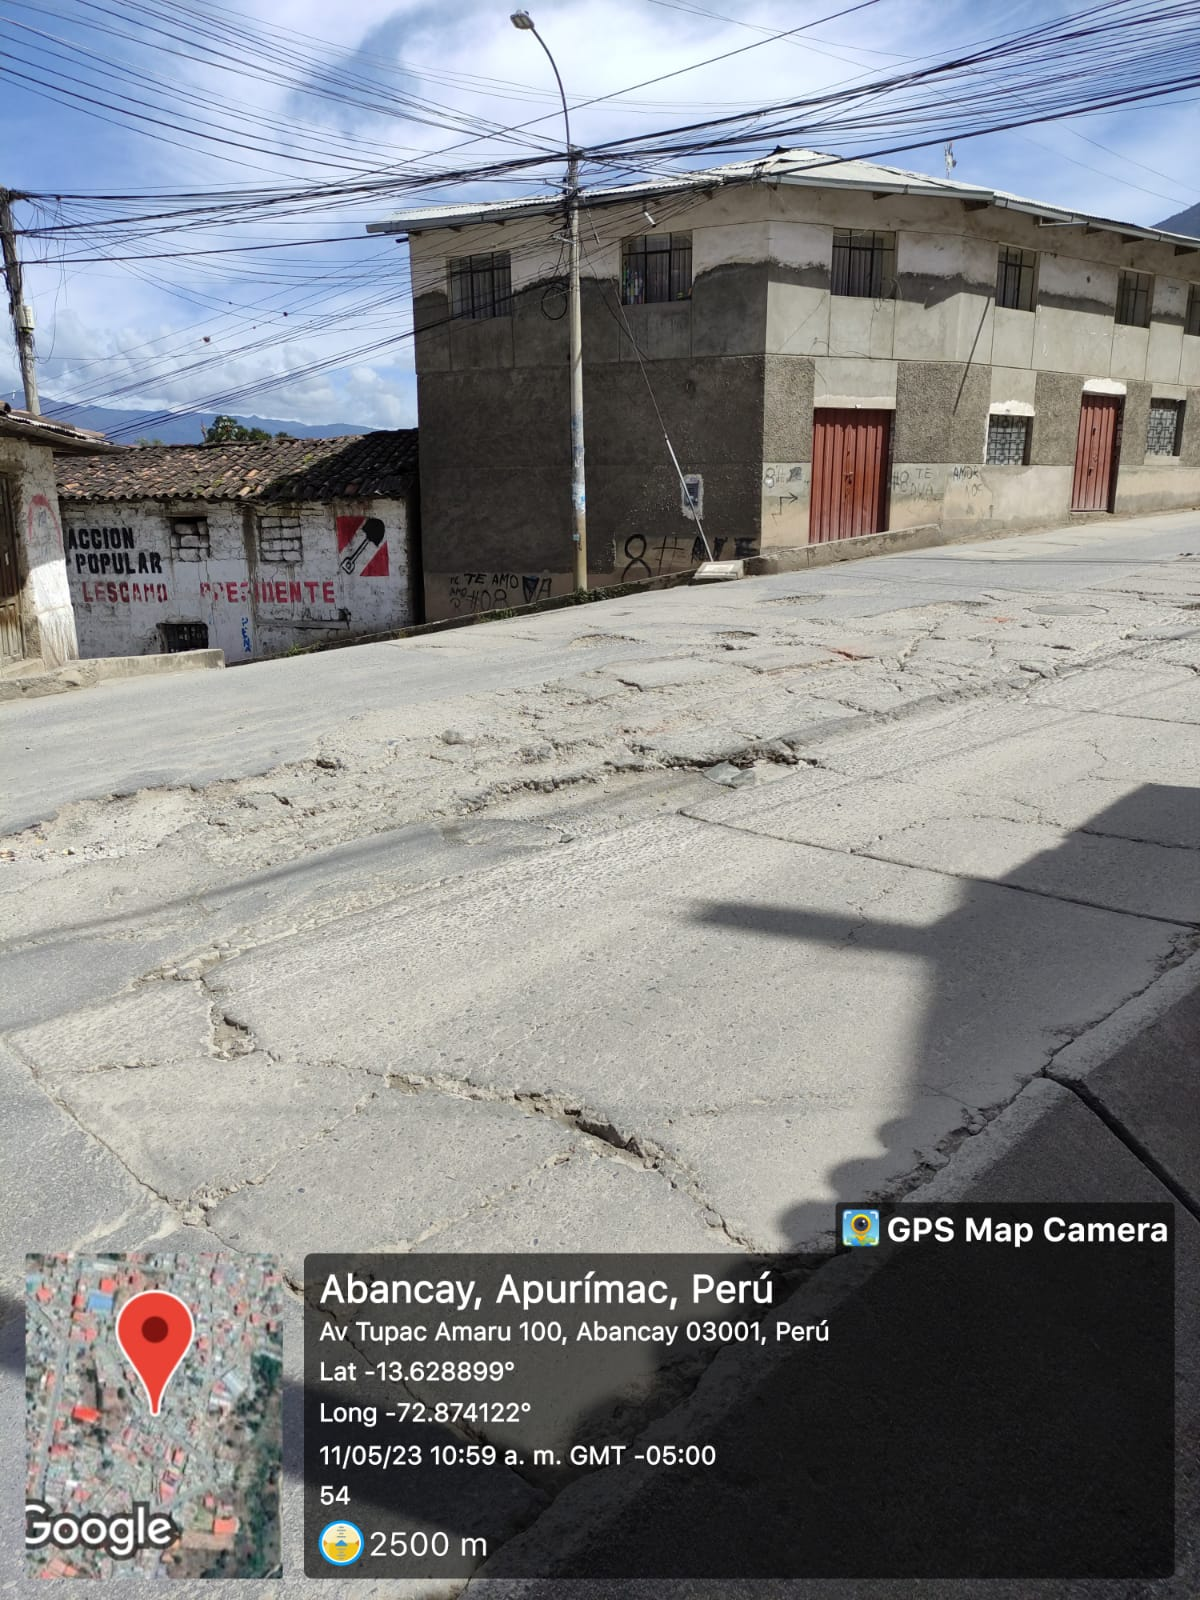
\includegraphics[width=\linewidth]{3.0.jpg}
		\caption{Intersección Av. Tupac Amaru con Av. Tamburco}
		\label{fig:subfigura1}
	\end{subfigure}
	\hfill
	\begin{subfigure}{0.45\textwidth}
		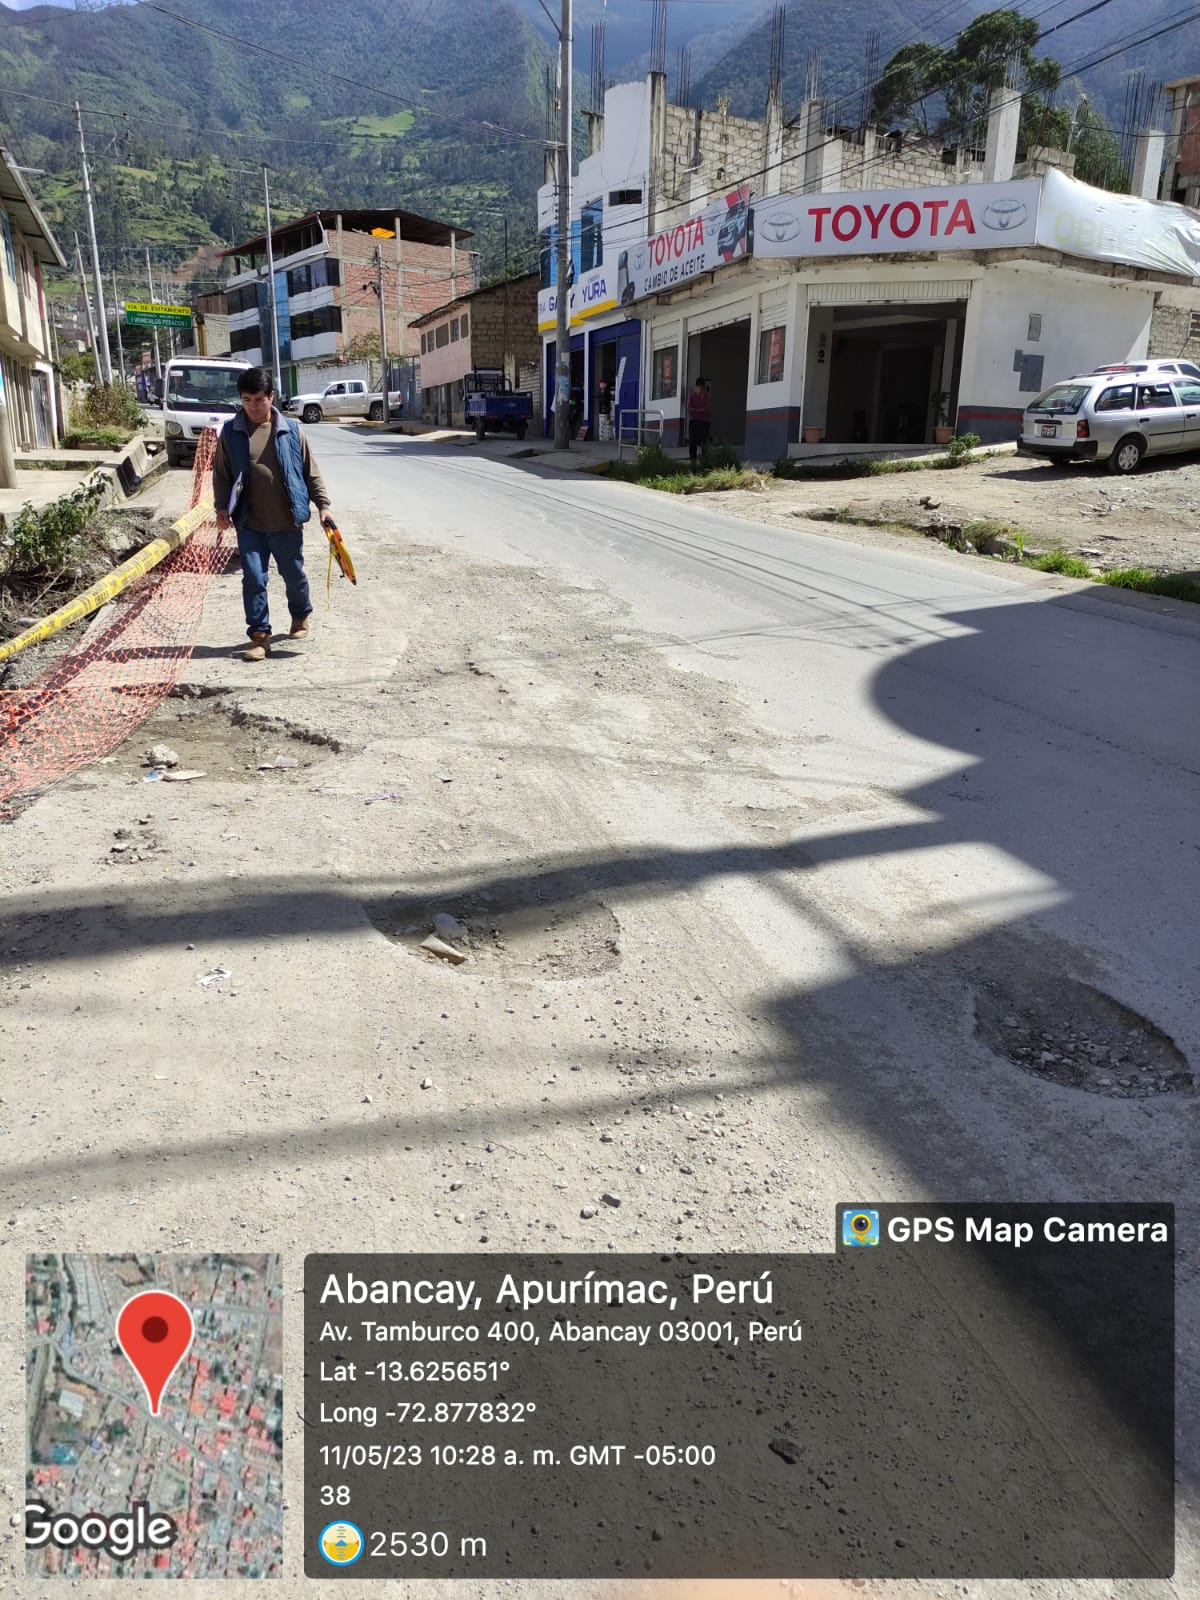
\includegraphics[width=\linewidth]{3.1.jpg}
		\caption{Intersección de Prolongación Huancavelica con Av. Tamburco}
		\label{fig:subfigura2}
	\end{subfigure}
	\caption{Se observa el desgaste y deterioro del pavimento flexible de la Av. Tamburco de causas no determinadas}
	\label{fig:ta-ph}
\end{figure}

\newpage
\begin{figure}[H]
	\begin{subfigure}{0.45\textwidth}
		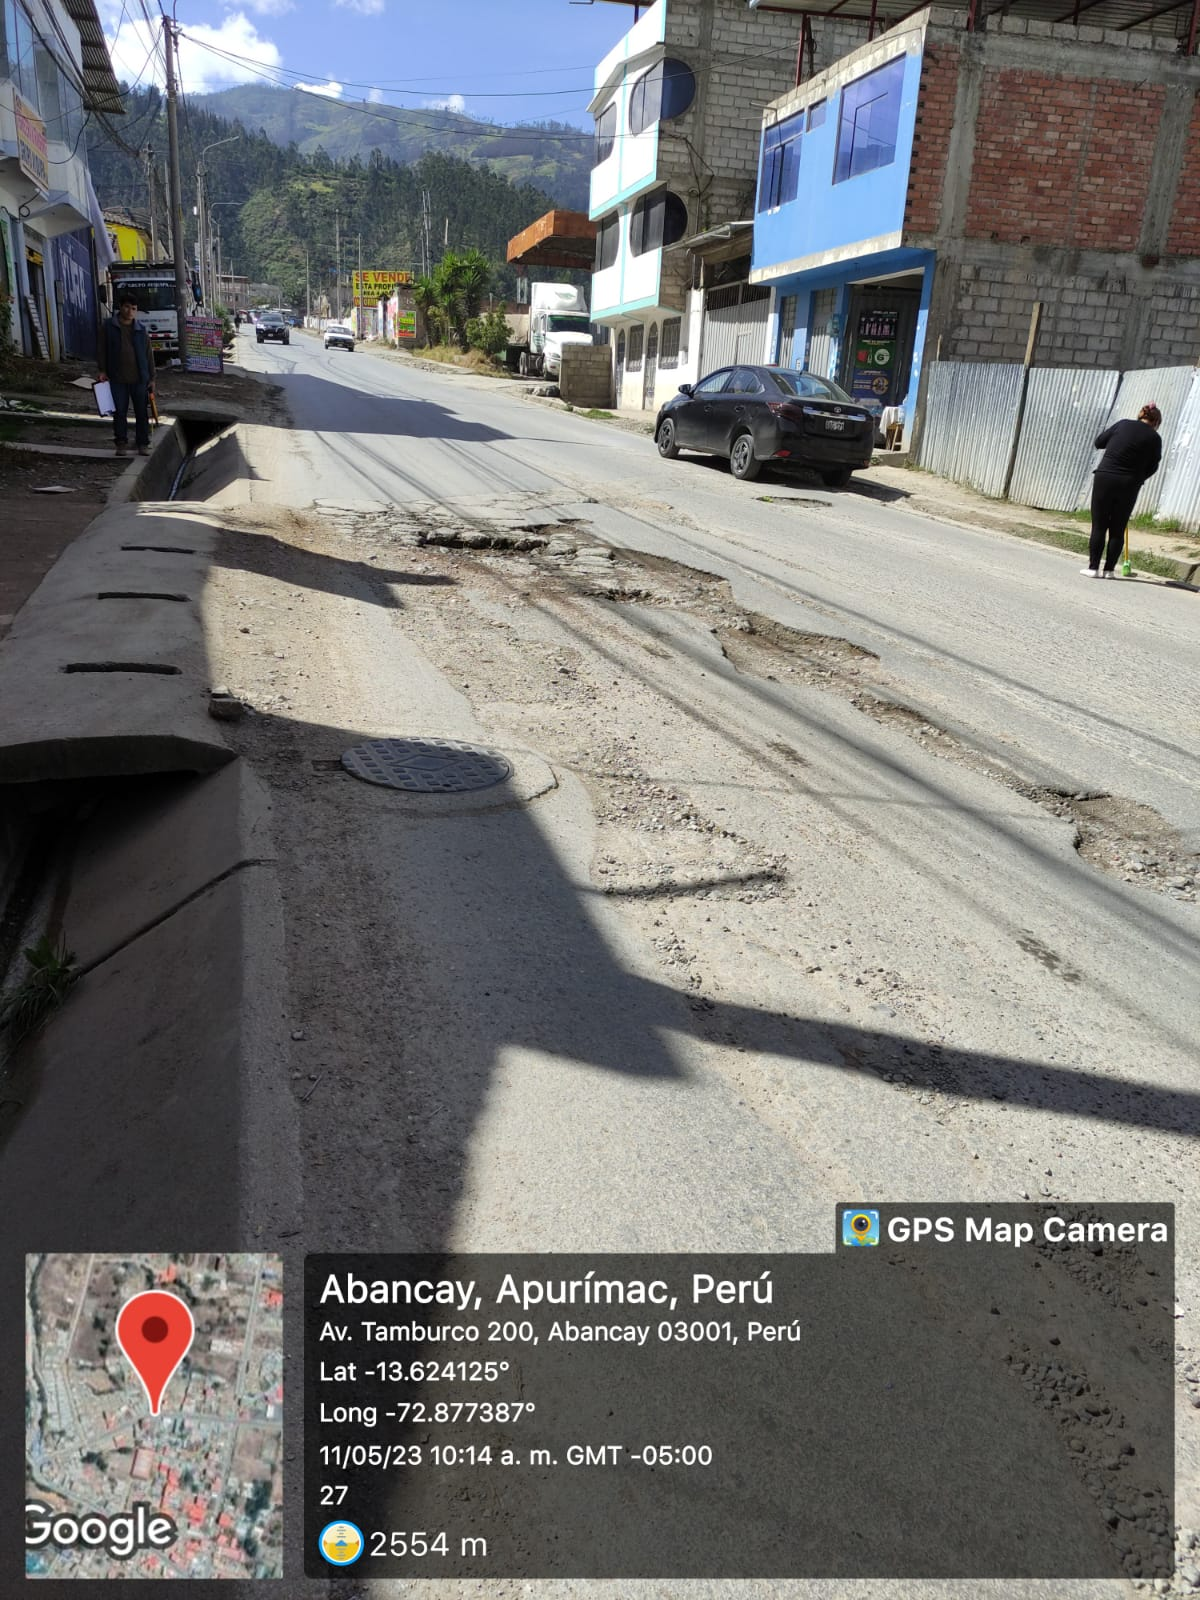
\includegraphics[width=\linewidth]{3.2.jpg}
		\caption{Intersección Jr. Arica con Av. Tamburco}
		\label{fig:subfigura3}
	\end{subfigure}
	\hfill
	\begin{subfigure}{0.45\textwidth}
		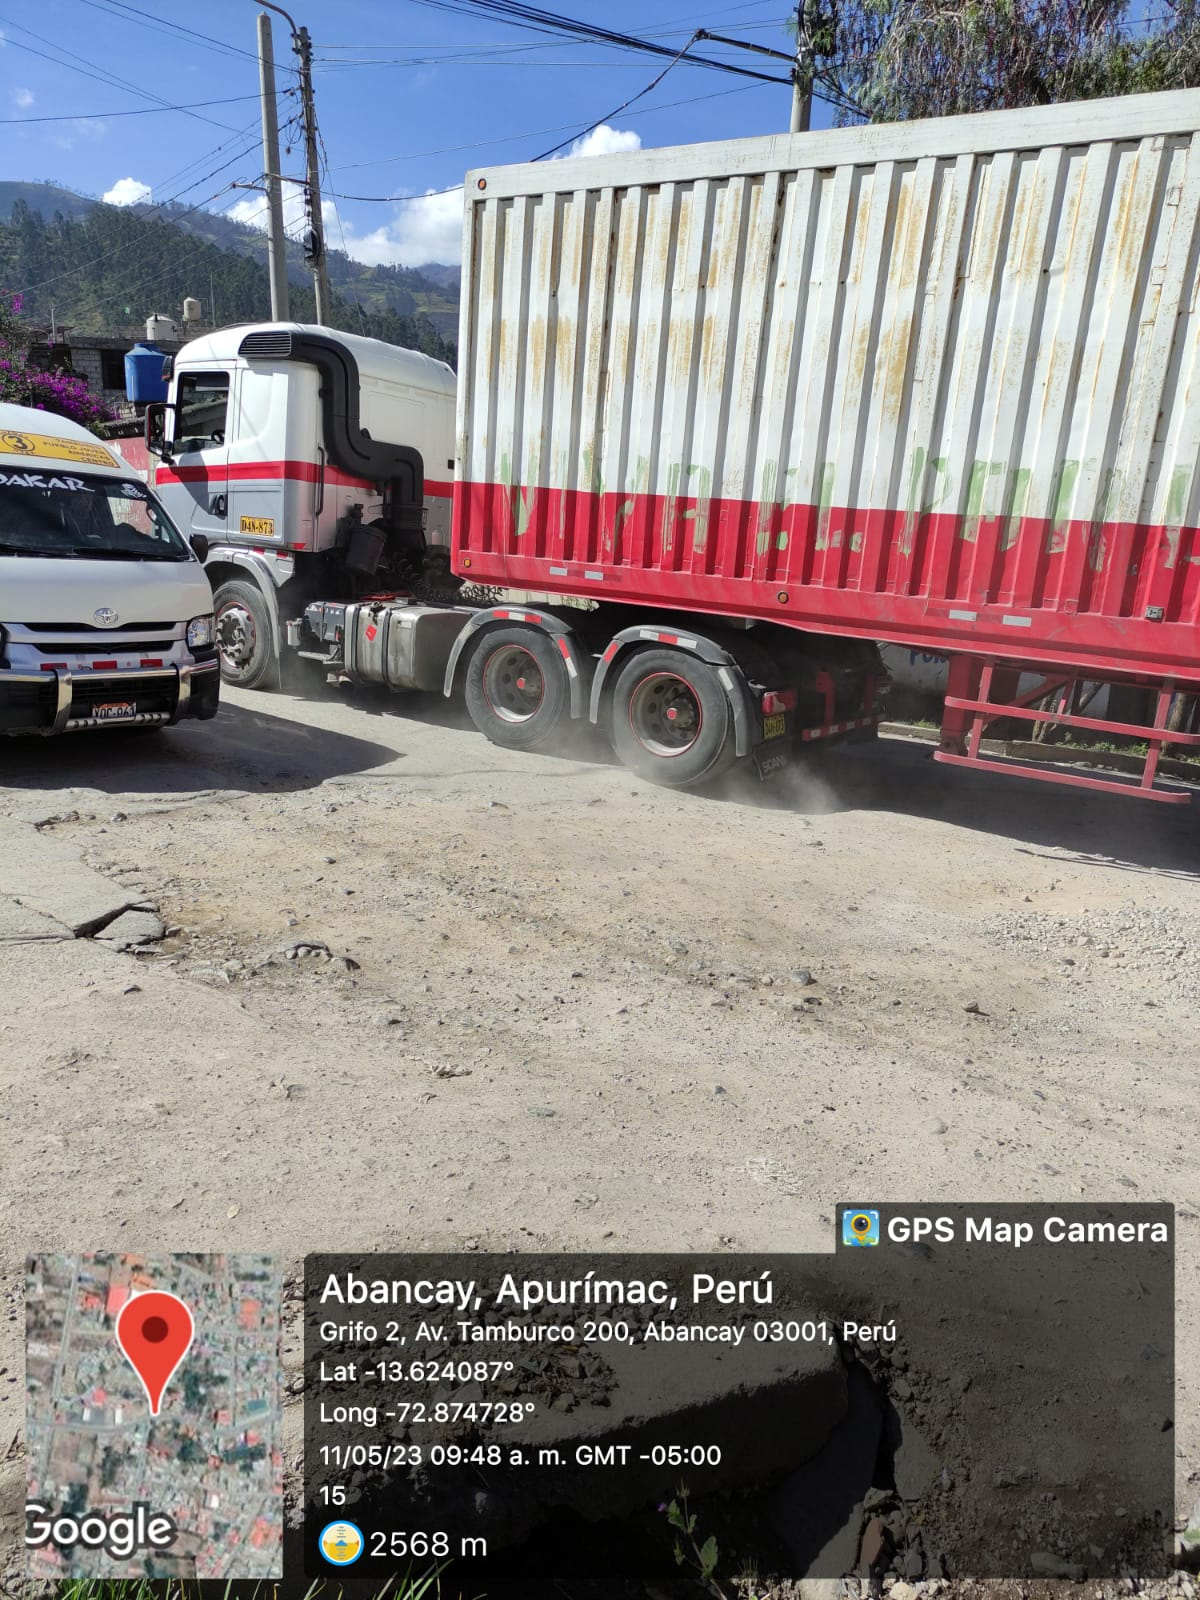
\includegraphics[width=\linewidth]{3.3.jpg}
		\caption{Intersección Av. Cononel Gonzales con Av. Tamburco}
		\label{fig:subfigura4}
	\end{subfigure}

	\caption{Se observa el desgaste y deterioro del pavimento flexible de la Av. Tamburco de causas no determinadas}
	\label{fig:at-cg}
\end{figure}

\section{Otras actividades realizadas}
\subsection{Trabajo de campo}

\begin{itemize}
	\item Se brindó apoyo en el levantamiento topográfico para la construcción de la Alameda en el sector conocido como Víctor Acosta. Este proceso involucró la medición y registro preciso de las características del terreno, proporcionando información detallada y crucial para el diseño y la ejecución de la obra. El levantamiento topográfico aseguró una planificación y construcción acorde con las condiciones reales del sitio, contribuyendo a la correcta implementación de la Alameda en el mencionado sector.
	\item Se procedió a la identificación y caracterización detallada del estado situacional del parque de la Plaza de Armas de Tamburco. Este proceso implicó un análisis minucioso de las condiciones actuales del espacio, incluyendo aspectos como el estado del pavimento, mobiliario urbano, áreas verdes, iluminación, entre otros. La recopilación de esta información proporcionó una base sólida para la planificación y ejecución de cualquier intervención o mejora que se requiera en el parque, garantizando así un espacio público óptimo y funcional para la comunidad de Tamburco.
	\item Se llevó a cabo la identificación exhaustiva del estado situacional del parque de diversiones "Señor de Exaltación". Este proceso incluyó un análisis detallado de las instalaciones, atracciones, infraestructura y condiciones generales del parque. Se recopilaron datos relevantes sobre el estado de conservación, seguridad, funcionamiento y aspectos estéticos. Esta evaluación proporcionó una base sólida para la toma de decisiones respecto a posibles mejoras, mantenimiento o renovaciones necesarias en el parque de diversiones "Señor de Exaltación", con el objetivo de asegurar un espacio recreativo óptimo y seguro para el disfrute de la comunidad.
	\item Se procedió con el trazo y replanteo para la cimentación de las estructuras que conformarán el techo del patio de honor del colegio Micaela Bastidas de Apurímac. Este proceso implicó la marcación precisa de los puntos y dimensiones necesarios para la correcta ubicación y nivelación de las bases de las estructuras. La meticulosidad en el trazado y replanteo aseguró que la cimentación se realizara de manera adecuada, proporcionando una base sólida y estable para la construcción del techo del patio de honor, contribuyendo así a la seguridad y durabilidad de la estructura.
	\item Se llevó a cabo el trazo y replanteo para la construcción del nivel Inicial de Nueva Rioja. Este proceso implicó la marcación precisa de puntos y dimensiones en el terreno, asegurando una ubicación y alineación adecuadas de la infraestructura. La meticulosidad en el trazado y replanteo garantizó que la construcción se llevara a cabo de manera precisa y conforme a los planos y diseños establecidos. Esto contribuyó a la creación de un entorno educativo seguro y funcional para los estudiantes del nivel Inicial en Nueva Rioja.
	\item Se procedió al metrado en campo para el acondicionamiento del Banco de la Nación en el Palacio Municipal de Tamburco. Este proceso implicó la medición detallada de las áreas y elementos que serían objeto de acondicionamiento, incluyendo aspectos como revestimientos, instalaciones, mobiliario y otros elementos relevantes para la adecuación del espacio. El metrado en campo proporcionó datos precisos y actualizados que sirvieron como base para la planificación y ejecución efectiva de las obras en el Banco de la Nación, asegurando así un ambiente funcional y apto para su uso en el Palacio Municipal de Tamburco.
	\item Se realizó el metrado detallado de las partidas necesarias para llevar a cabo el mantenimiento del Palacio Municipal de Tamburco. Este proceso implicó la medición precisa de cada elemento y actividad requerida, abarcando aspectos como revestimientos, instalaciones, pintura, carpintería, entre otros. El metrado proporcionó una estimación cuantitativa y cualitativa de los materiales y recursos necesarios para la ejecución efectiva del plan de mantenimiento, contribuyendo a una gestión eficaz de los recursos y garantizando la conservación y óptimo funcionamiento del Palacio Municipal de Tamburco.
\end{itemize}

\subsection{Trabajo en gabinete}
\begin{itemize}
	\item Se llevó a cabo el procesamiento de los puntos crudos del sector conocido como Víctor Acosta utilizando el software Civil 3D 2024. Se procedió con el modelamiento detallado de la superficie, la definición del alineamiento y la creación de la sección típica, dando lugar a la generación del "corridor". A partir de este modelo, se cuantificó el volumen de corte y relleno necesario para la construcción de la infraestructura en esta zona. Este proceso, realizado con herramientas de vanguardia, garantizó una planificación y ejecución precisa y eficaz de la obra en el sector Víctor Acosta, asegurando una implementación óptima y funcional de la infraestructura.
	\item Se ha elaborado un informe detallado sobre el estado actual del parque situado en la Plaza de Armas de Tamburco. En este informe se identificaron y detallaron los activos que se encuentran en mal estado, tomando en consideración que el parque ya había sido intervenido durante la gestión anterior. Este análisis exhaustivo proporciona una visión clara de los elementos que requieren atención y posible renovación, permitiendo una planificación efectiva para mejorar y mantener este espacio público importante para la comunidad de Tamburco.
	\item Se ha generado un reporte exhaustivo del estado actual del parque de diversiones "Señor de Exaltación". Se realizó el metrado de las partidas siguiendo la normativa establecida en la Norma Técnica de Metrados para obras de Edificación y Habilitaciones Urbanas, aprobada por el Ministerio de Vivienda, Construcción y Saneamiento en el año 2010 \cite{MVCS2010}. Esta normativa proporciona los lineamientos y criterios para la medición de los diferentes elementos y actividades involucradas en la construcción y habilitación urbana. El reporte incluye detalles sobre las unidades y criterios utilizados en el metrado, proporcionando una base sólida para la planificación y ejecución de las intervenciones necesarias en el parque "Señor de Exaltación".
	\item Se llevó a cabo el replanteo para la cimentación de las estructuras que conformarán el soporte del techo del patio de honor del Colegio Micaela Bastidas, utilizando el software de dibujo asistido por computadora AutoCAD 2024. Este proceso implicó la utilización de herramientas precisas y avanzadas para asegurar la correcta ubicación y alineación de las bases de las estructuras. El uso de AutoCAD 2024 garantizó un replanteo preciso y eficaz, proporcionando una base sólida para la construcción del soporte del techo, contribuyendo así a la seguridad y durabilidad de la estructura en el patio de honor del Colegio Micaela Bastidas.
	\item RSe procedió con el replanteo del perímetro para la construcción del nivel Inicial en Nueva Rioja. El trabajo consistió en el dibujo preciso del perímetro de la propiedad de este centro educativo utilizando el software de dibujo asistido por computadora AutoCAD 2024. Este proceso permitió establecer de manera exacta los límites de la propiedad, brindando una base sólida y confiable para la ejecución de la construcción. La utilización de AutoCAD 2024 garantizó un replanteo preciso y eficiente, contribuyendo a la correcta ubicación y alineación de la infraestructura educativa en Nueva Rioja.
	\item Se brindó apoyo en la redacción de especificaciones técnicas y memorias descriptivas para el acondicionamiento del Banco de la Nación en el Palacio Municipal. Para ello, se utilizó el sistema de composición de textos \LaTeX, reconocido por su capacidad para crear documentos con una alta calidad tipográfica y estructural. Este enfoque aseguró la generación de documentos escritos de alto estándar, proporcionando una presentación clara y profesional de los detalles técnicos y descriptivos necesarios para la realización del proyecto de acondicionamiento.
	\item Se llevaron a cabo los metrados necesarios para el proyecto. Para este fin, se realizó el modelado detallado en el software Revit 2024. Esta herramienta permitió una representación tridimensional precisa y completa del futuro estado del sótano del Palacio Municipal, incluyendo las instalaciones sanitarias, especiales, área de atención al usuario y accesos. El modelado en Revit facilitó la cuantificación exacta de los materiales y recursos requeridos, proporcionando una base sólida para la planificación y ejecución del proyecto de remodelación.
	\item Se llevó a cabo la programación detallada de la obra para este proyecto, utilizando el software especializado en gestión de proyectos Oracle Primavera P6. Esta herramienta permitió establecer una planificación precisa y cronograma de actividades, asignando recursos y tiempos de ejecución de manera eficiente. La utilización de Oracle Primavera P6 garantizó un seguimiento y control riguroso del progreso de la obra, facilitando la toma de decisiones y asegurando la ejecución exitosa y en tiempo del proyecto de remodelación del sótano del Palacio Municipal.
	\item  Se brindó apoyo en la programación detallada de la obra para el mantenimiento del Palacio Municipal de Tamburco. Para ello, se utilizó herramientas especializadas que permitieron establecer un cronograma preciso de actividades, asignando recursos y tiempos de ejecución de manera eficiente. Esta programación facilitó un seguimiento riguroso del progreso de la obra, contribuyendo a una gestión efectiva y exitosa del mantenimiento del Palacio Municipal de Tamburco.
\end{itemize}

Es notable destacar que, para cualquier consulta, se contó con la disponibilidad y colaboración de todo el equipo de la Oficina de Obras perteneciente a la Sub-Gerencia de la Municipalidad Distrital de Tamburco. Esta apertura y disposición del personal evidencia un ambiente de trabajo colaborativo y una cultura organizativa orientada hacia la eficiencia y la cooperación en pos de los objetivos comunes.
\newpage
\subsection{Panel fotográfico de otras actividades realizadas}
\begin{figure}[h]
	\captionsetup{width=0.8\textwidth}
	\centering
	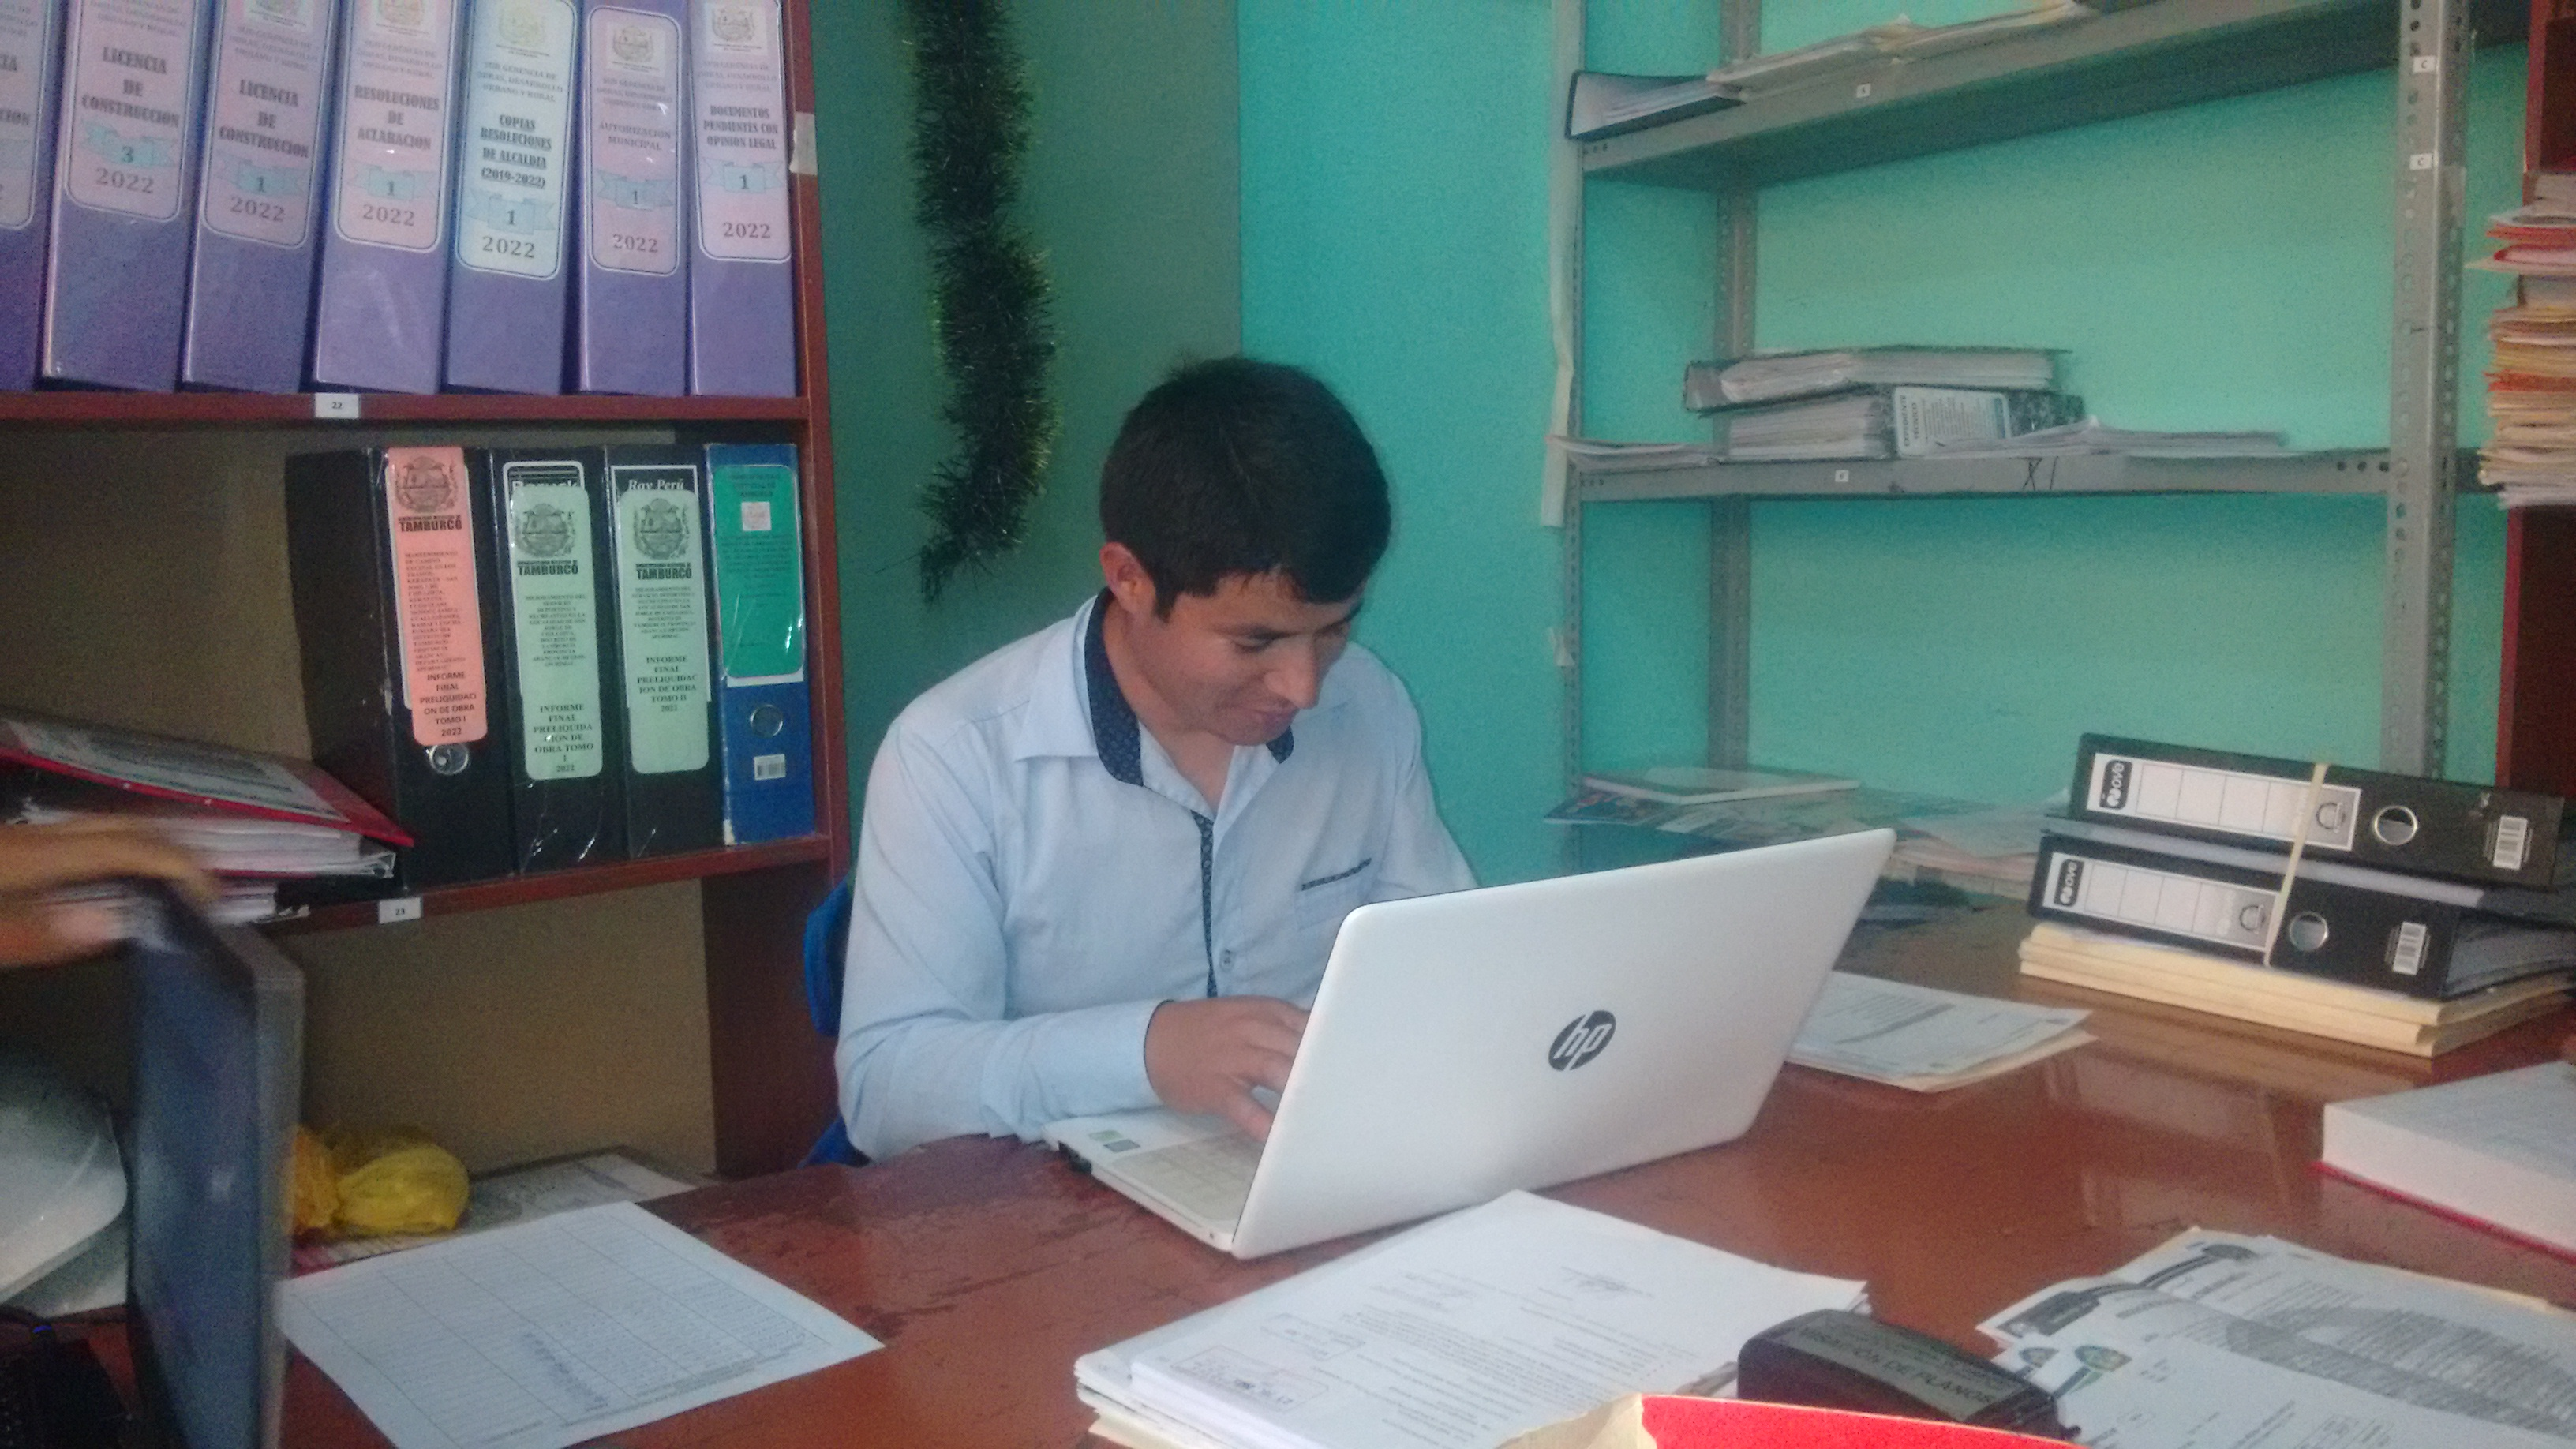
\includegraphics[width=0.8\linewidth]{3.18.jpg}
	\caption[Trabajos realizados en gabinete]{Trabajos realizados en gabinete de la oficina de obras de la Municipalidad Distrital de Tamburco}
	\label{fig:img20230825125748803}
\end{figure}

\begin{figure}[h]
	\captionsetup{width=0.8\textwidth}
	\centering
	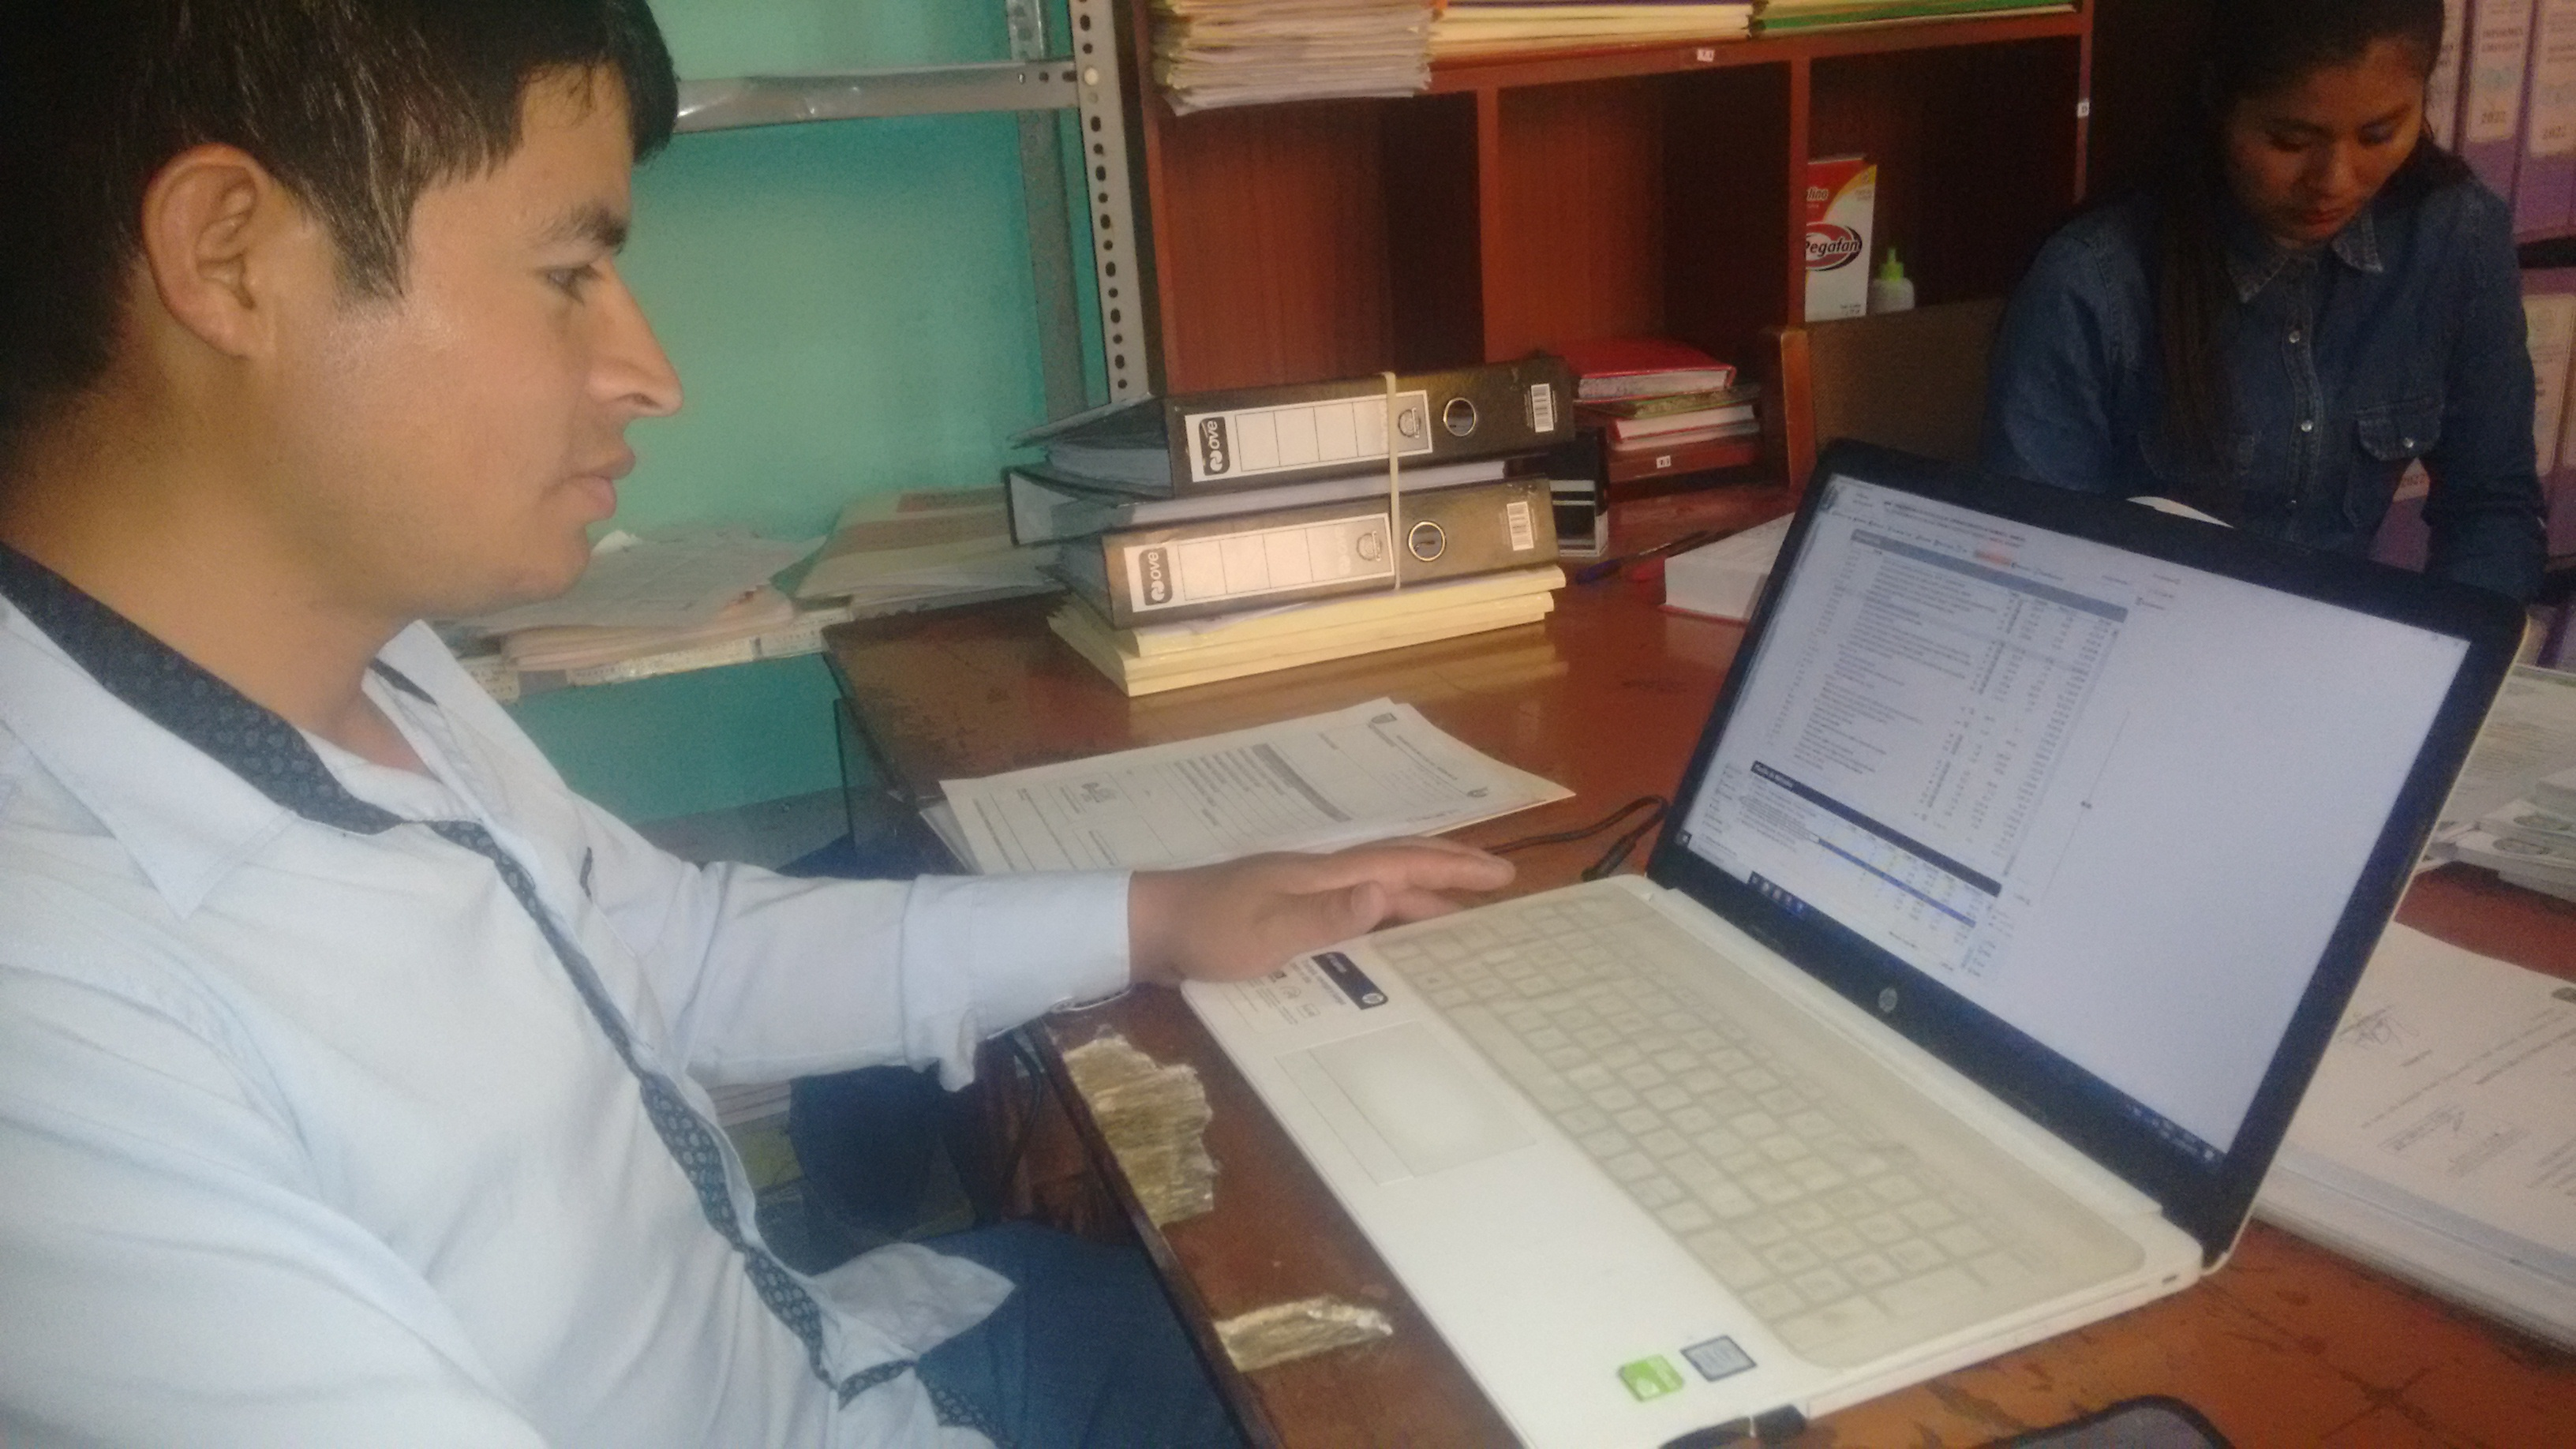
\includegraphics[width=0.8\linewidth]{3.4.jpg}
	\caption[Trabajo en gabinete: Uso del software Power Cost]{Trabajo en gabinete, utilizando el software de costos y presupuestos denominado Power Cost.}
	\label{fig:img20230825131400193}
\end{figure}

\begin{figure}[h]
	\captionsetup{width=0.8\textwidth}
	\centering
	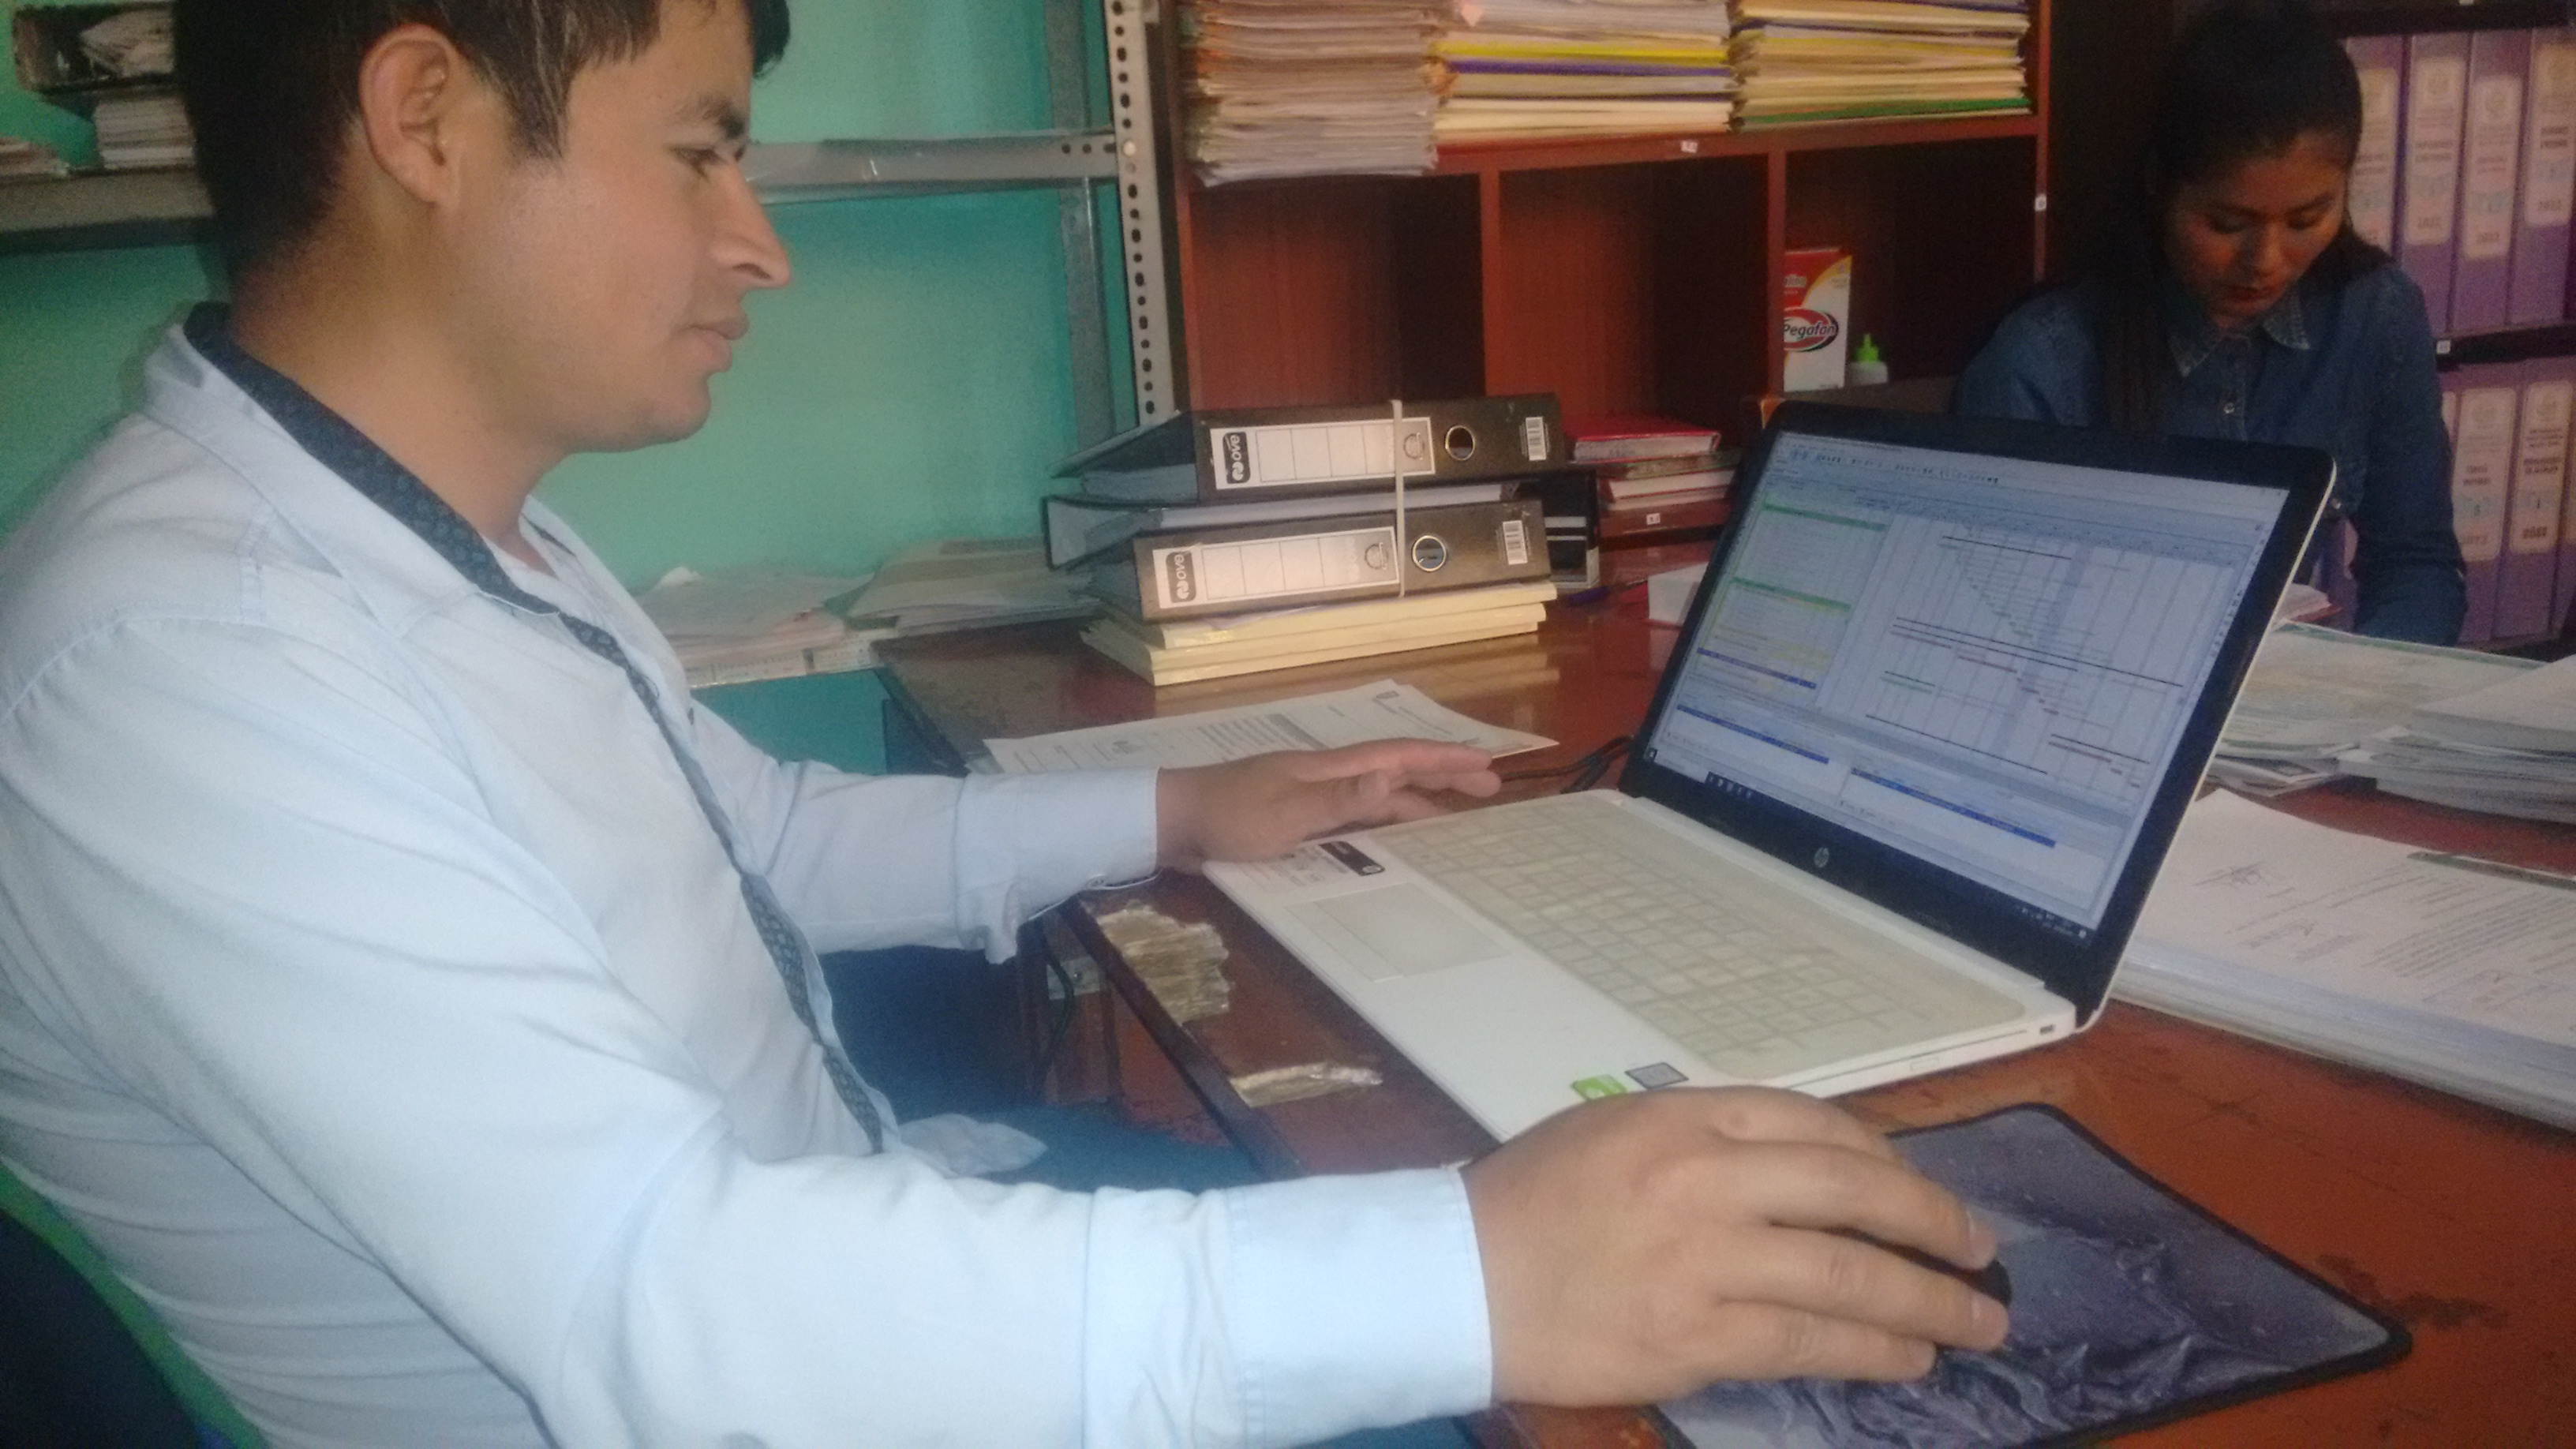
\includegraphics[width=0.8\linewidth]{3.5.jpg}
	\caption[Trabajo en gabinete: Uso del software Oracle Primavera]{Trabajo del gabinete utilizando el software de planificación y control de proyectos Oracle Primavera P6 .}
	\label{fig:img20230825131405944}
\end{figure}

\begin{figure}[h]
	\captionsetup{width=0.8\textwidth}
	\centering
	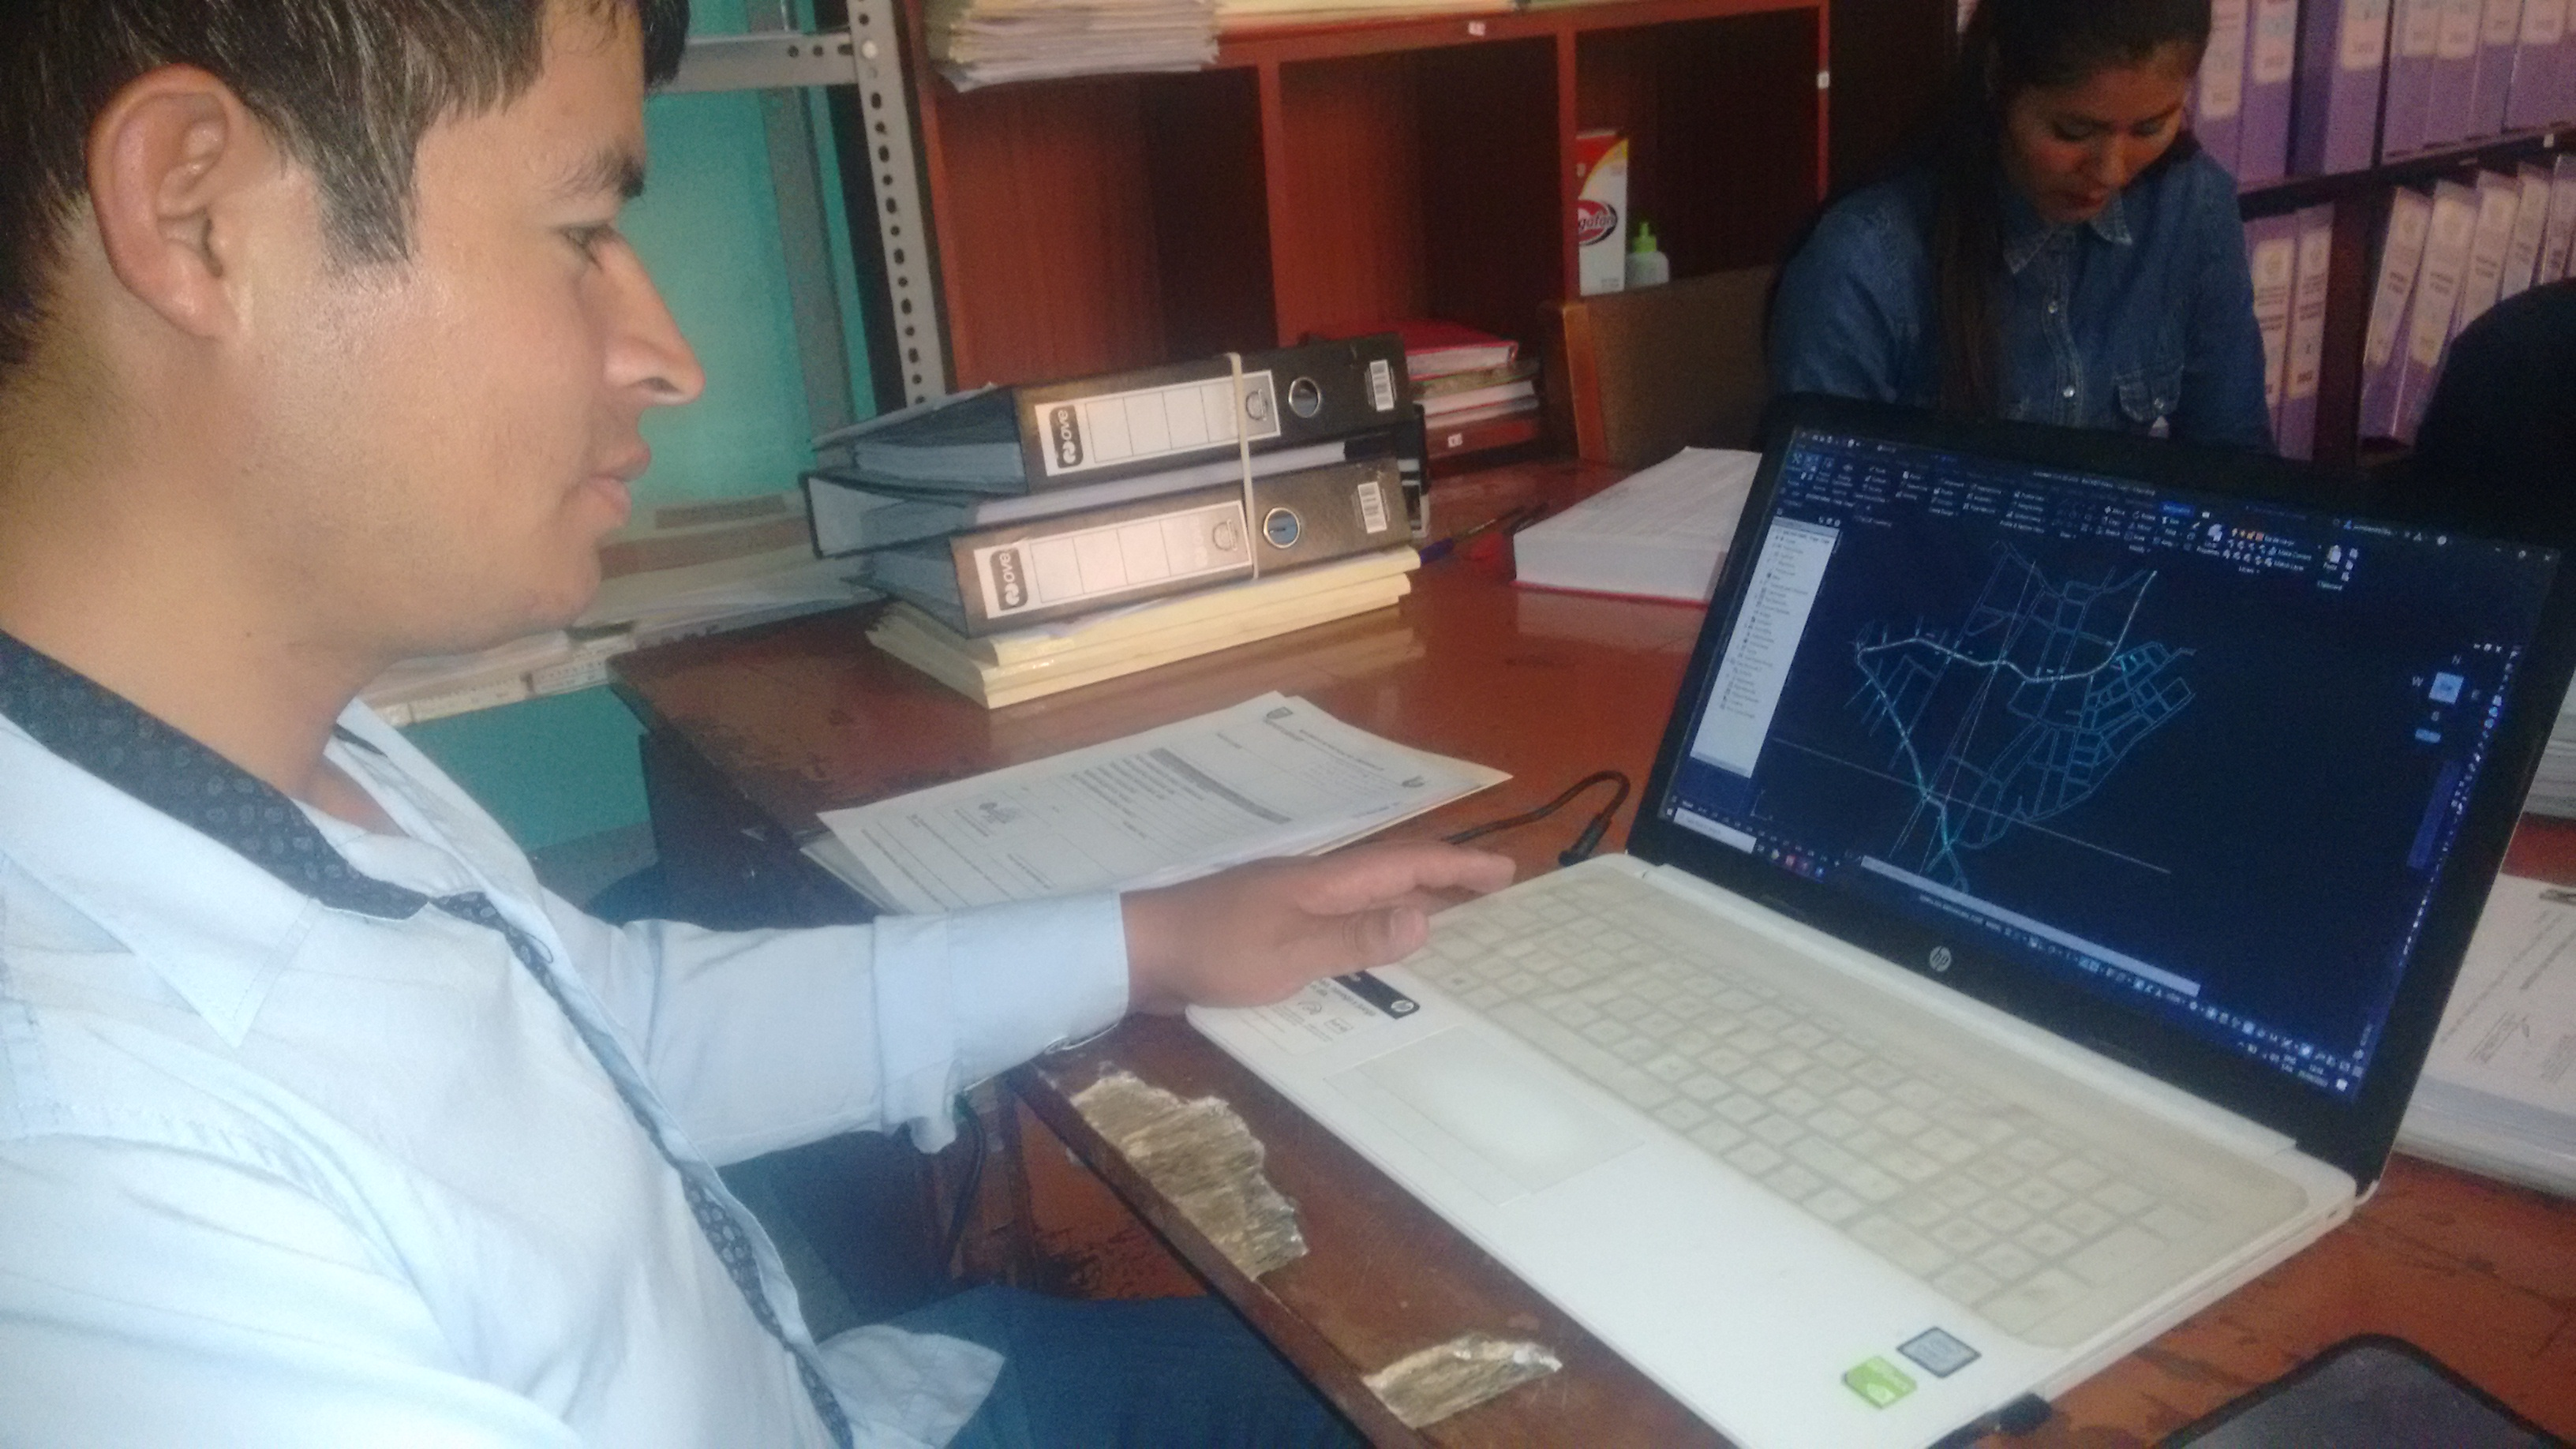
\includegraphics[width=0.8\linewidth]{3.6.jpg}
	\caption[Trabajo de gabinete: Uso del software Civil 3D 2024]{Trabajo del gabinete:Modelamiento de la Av. Tamburco, utilizando el software Civil 3D 2024}
	\label{fig:img20230825131413779}
\end{figure}

\begin{figure}[h]
	\captionsetup{width=0.8\textwidth}
	\centering
	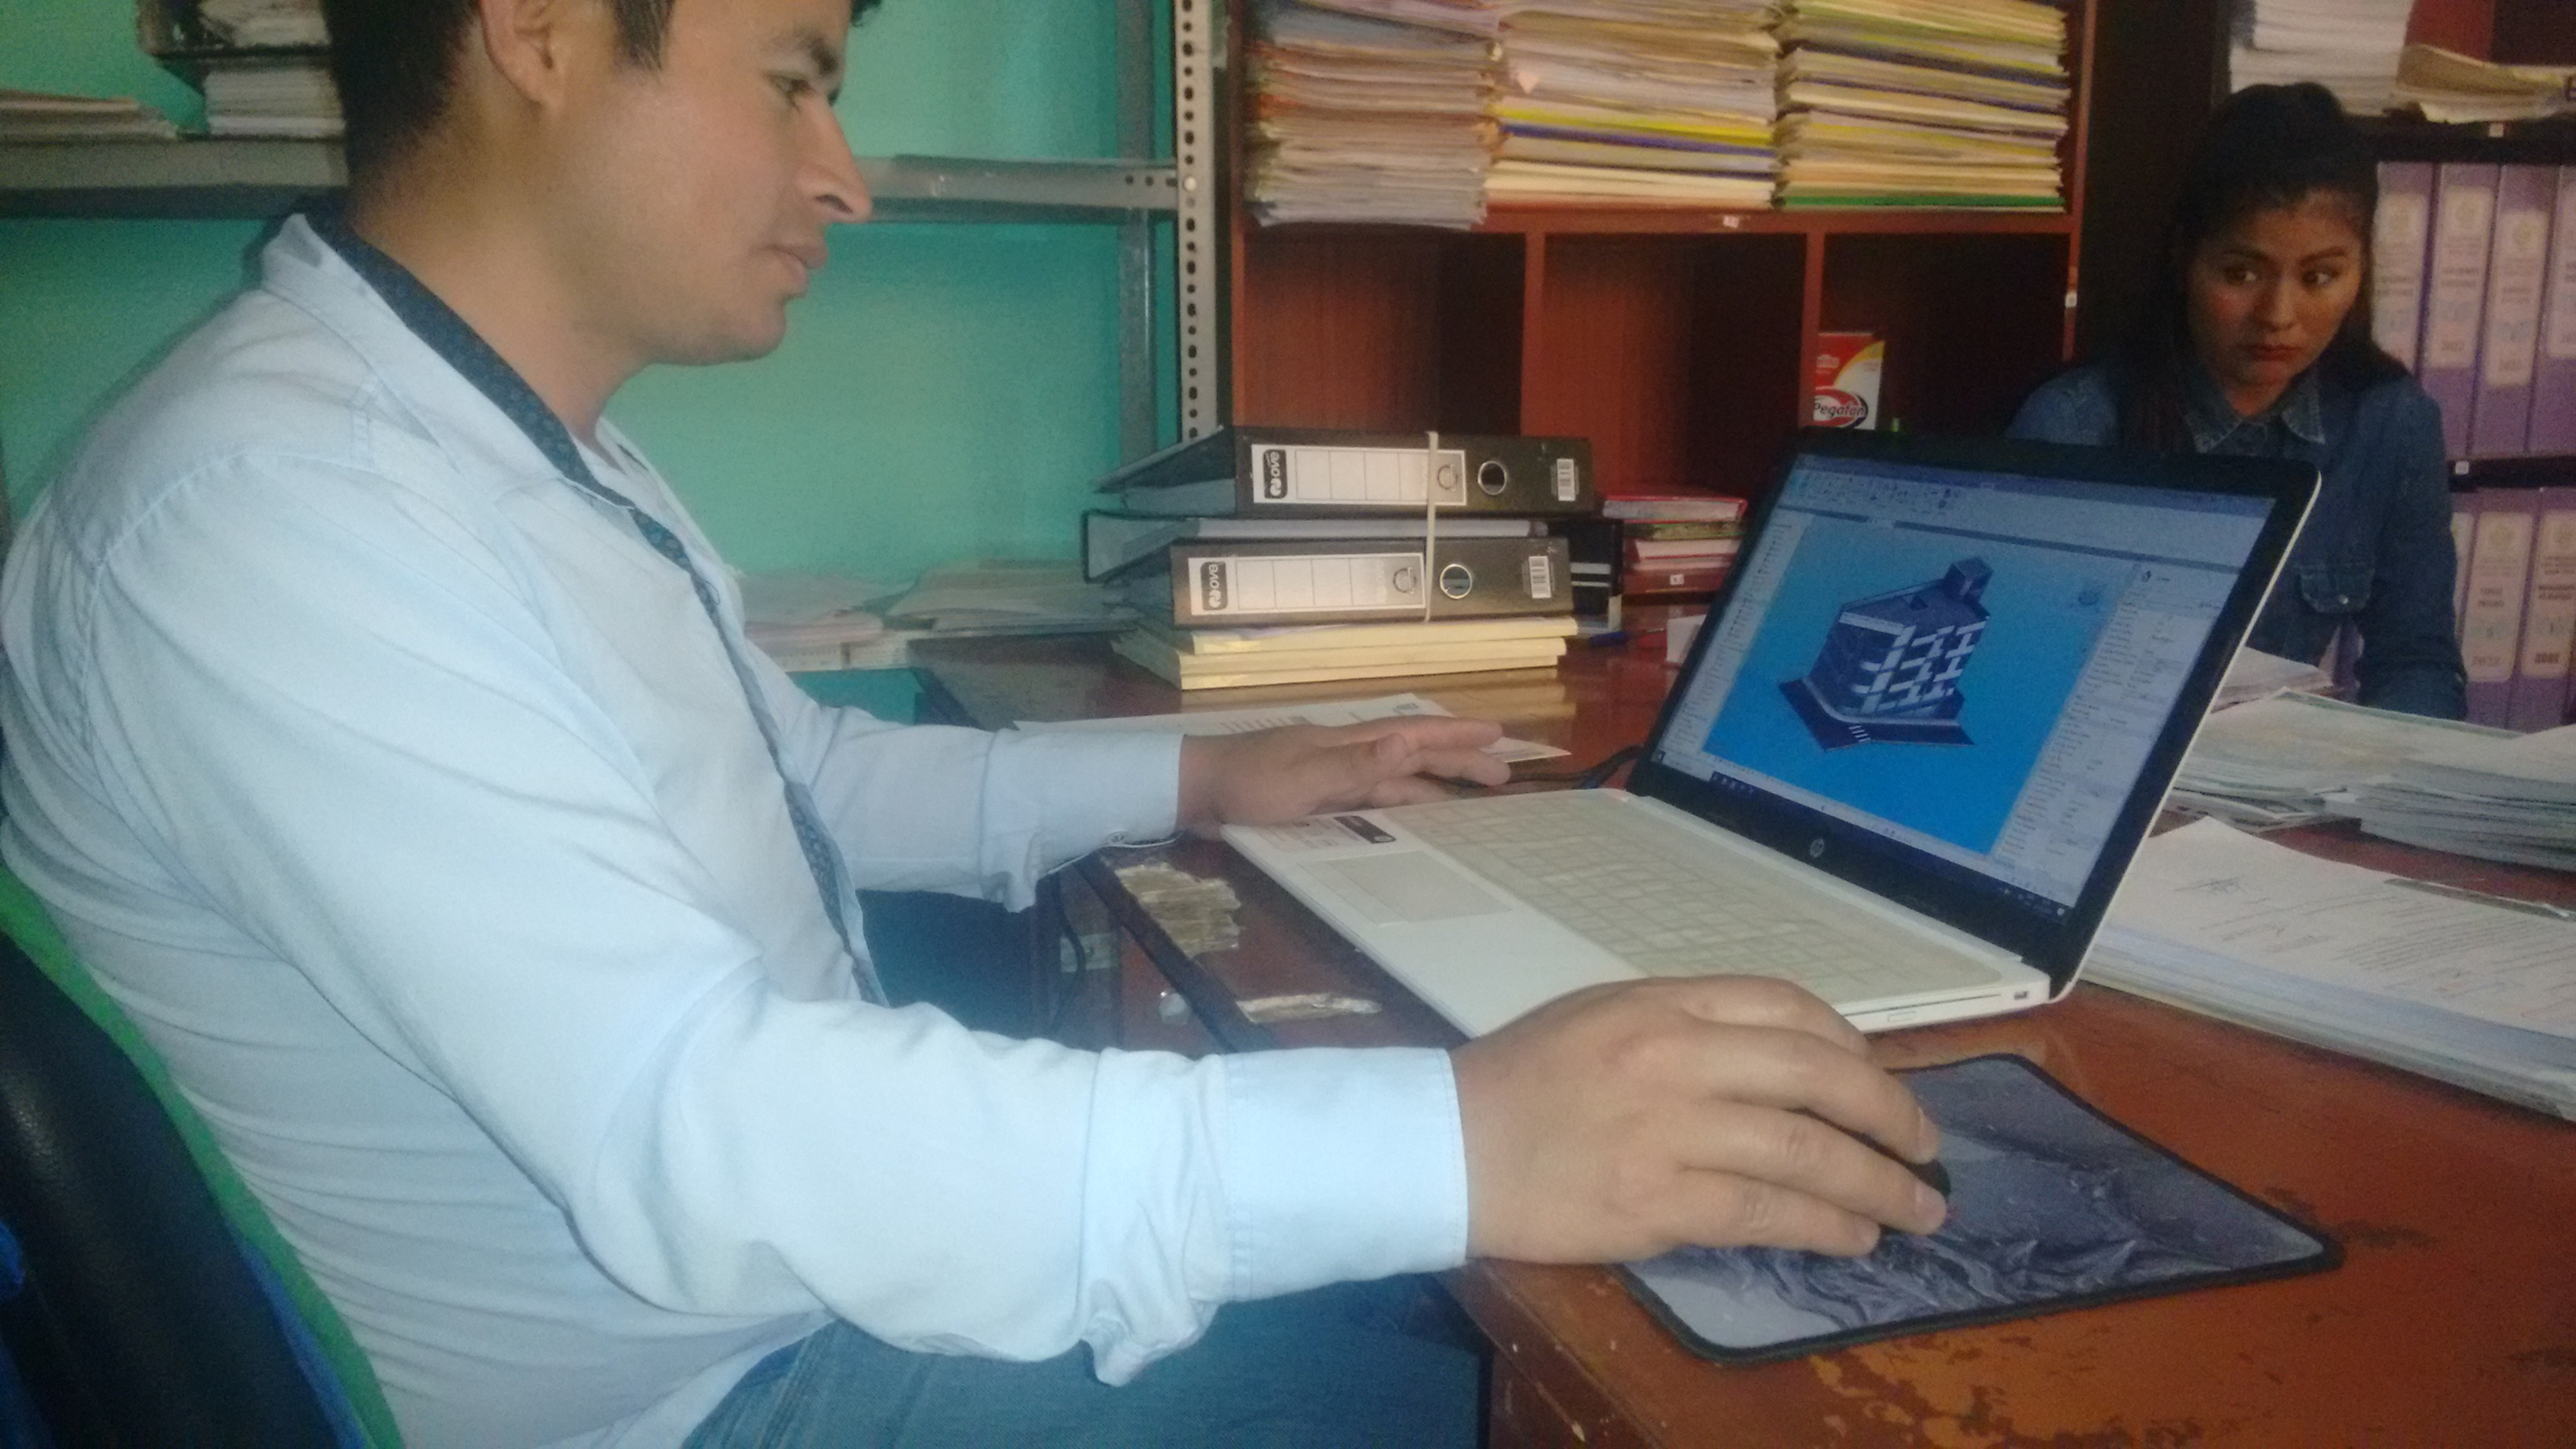
\includegraphics[width=0.8\linewidth]{3.7.jpg}
	\caption[Trabajo en gabinete: Modelamiento del Palacio Municipal de Tamburco utilizando Revit 2024]{Modelamiento del Palacio de la Municipalidad Distrital de Tamburco, para el acondicionamiento de la sede del Banco de la Nación, utilizando el software Revit 2024}
	\label{fig:img20230825131426665}
\end{figure}


\begin{figure}[h]
	\captionsetup{width=0.8\textwidth}
	\centering
	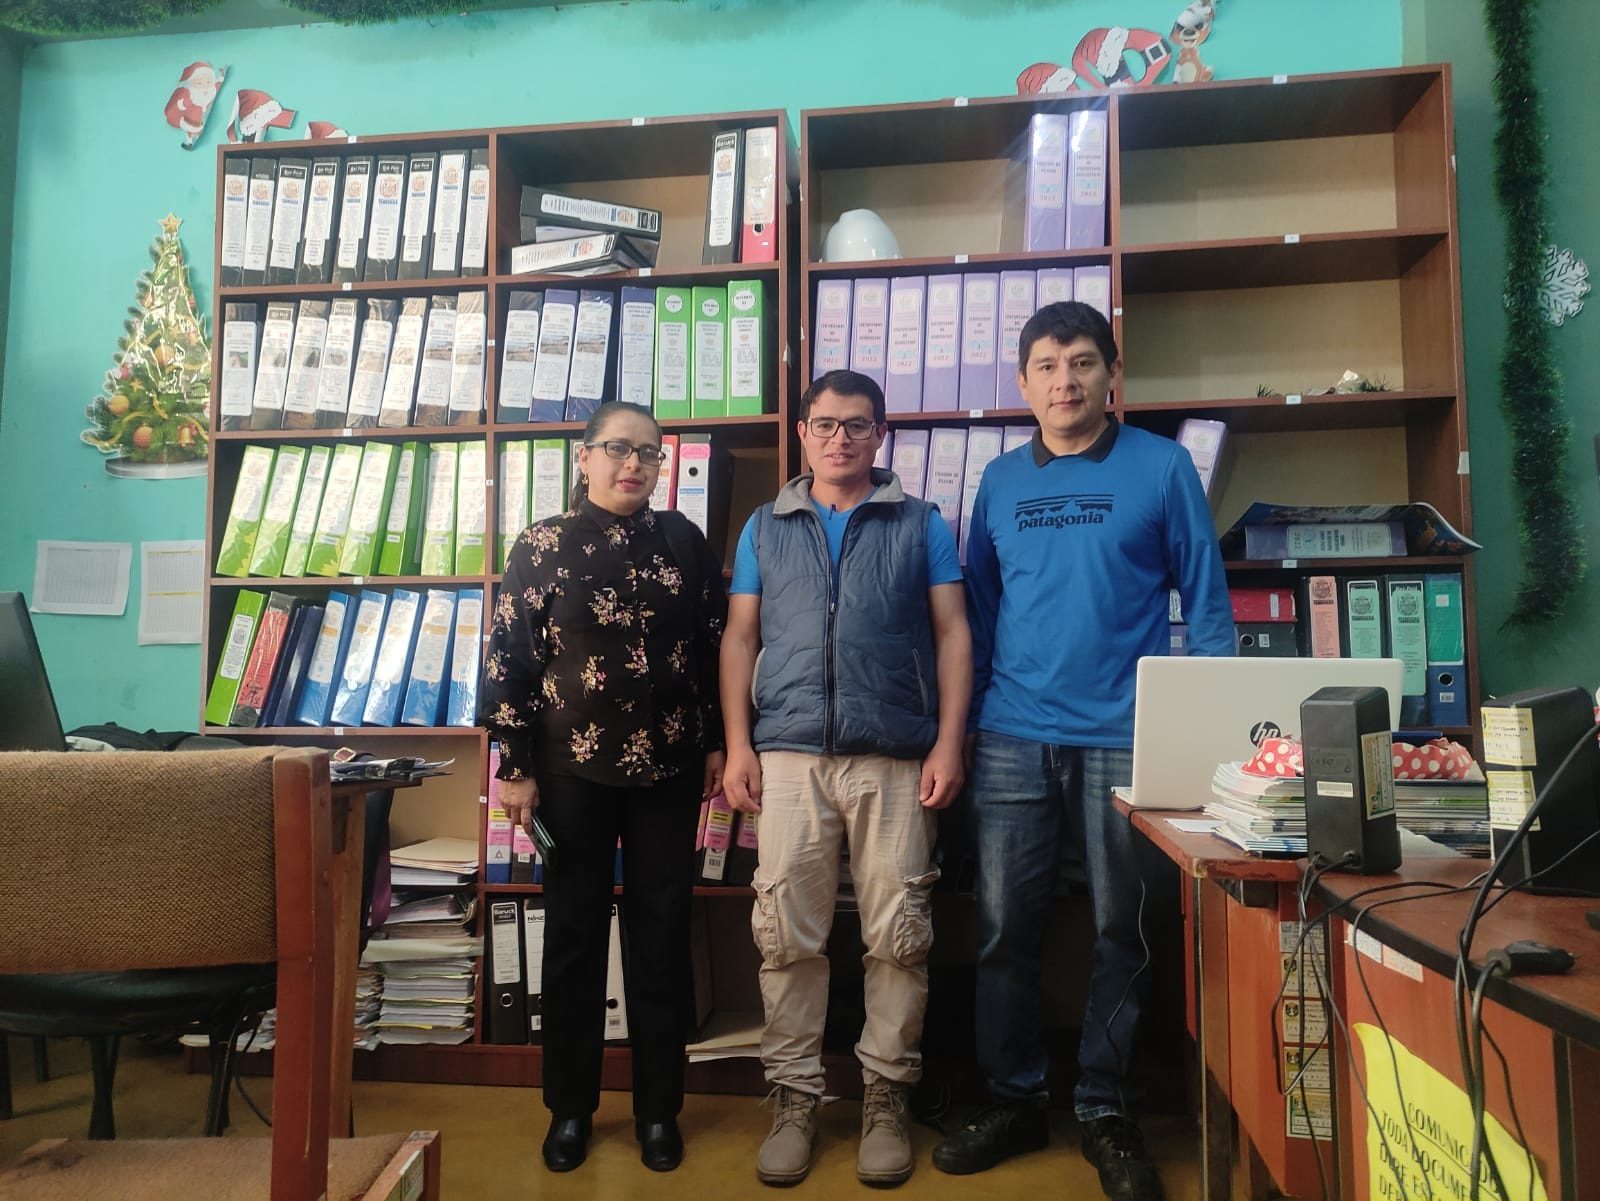
\includegraphics[width=0.8\linewidth]{3.11.png}
	\caption[Visita de la asesora de prácticas]{En la imagen se observa en la izquierda a la Dra. Lucy M. Guanuchi Orellana, en la derecha el Sub-Gerente de Obras de la Municipalidad Distrital de Tamburco y en el centro el practicante.}
	\label{fig:visita-de-la-asesora-2}
\end{figure}

\begin{figure}[h]
	\captionsetup{width=0.8\textwidth}
	\centering
	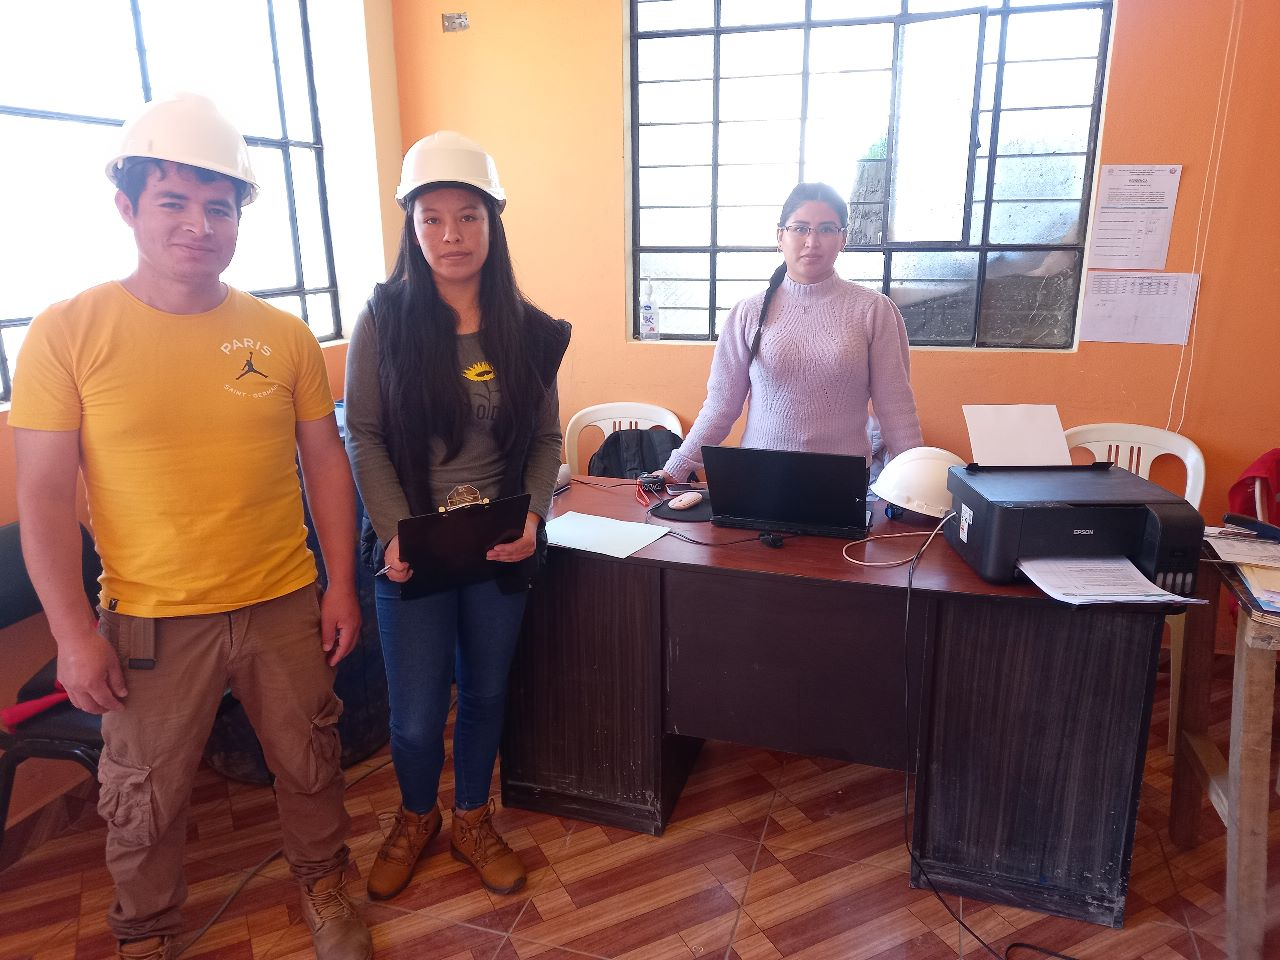
\includegraphics[width=0.8\linewidth]{3.19.jpg}
	\caption[Visita inopinada a las diferentes obras ejecutadas por la Municipalidad Distrital de Tamburco]{Visita inopinada por parte de la sub-gerencia de obras a las diferentes obras de la Municipalidad Distrital de Tamburco}
	\label{fig:1}
\end{figure}

\begin{figure}[h]
	\captionsetup{width=0.8\textwidth}
	\centering
	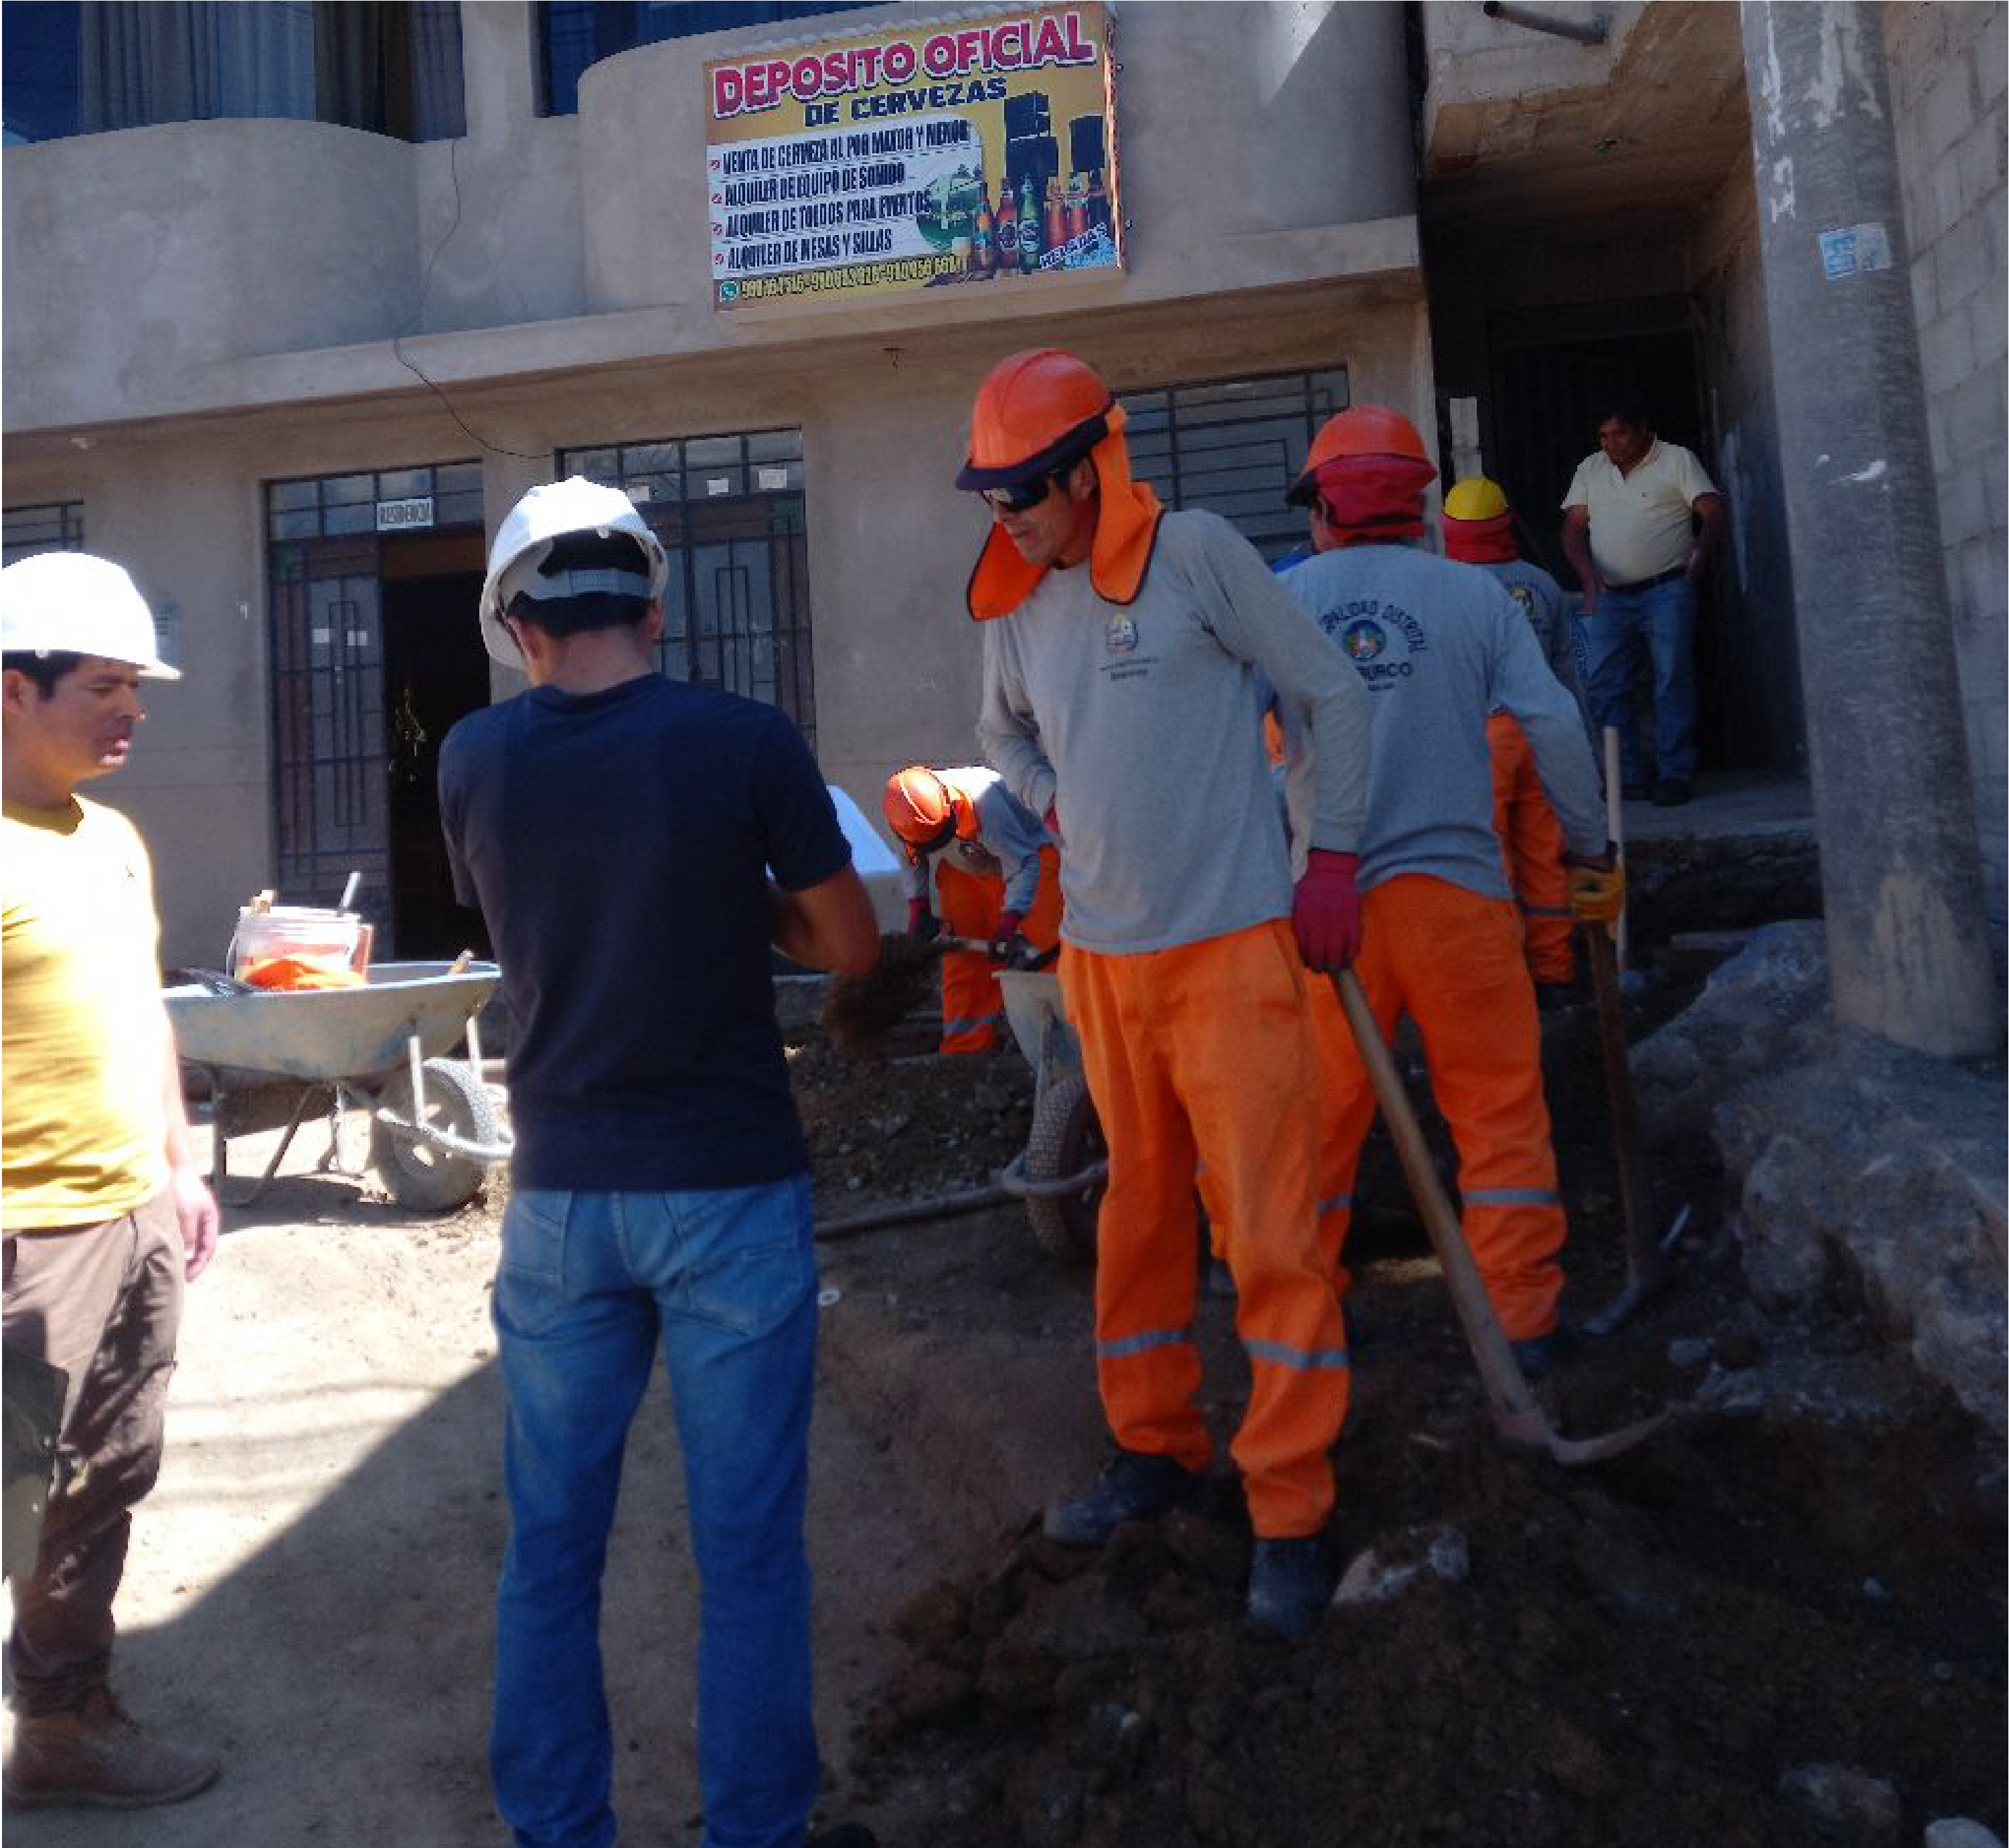
\includegraphics[width=0.8\linewidth]{3.9.png}
	\caption[Visita a obras en ejecución]{Visita al sector de Socoshuayco, donde se viene ejecutando las obras de pavimentación de pistas y veredas}
	\label{fig:visita-a-campo}
\end{figure}

\begin{figure}[h]
	\captionsetup{width=0.8\textwidth}
	\centering
	\begin{adjustbox}{angle=90}
	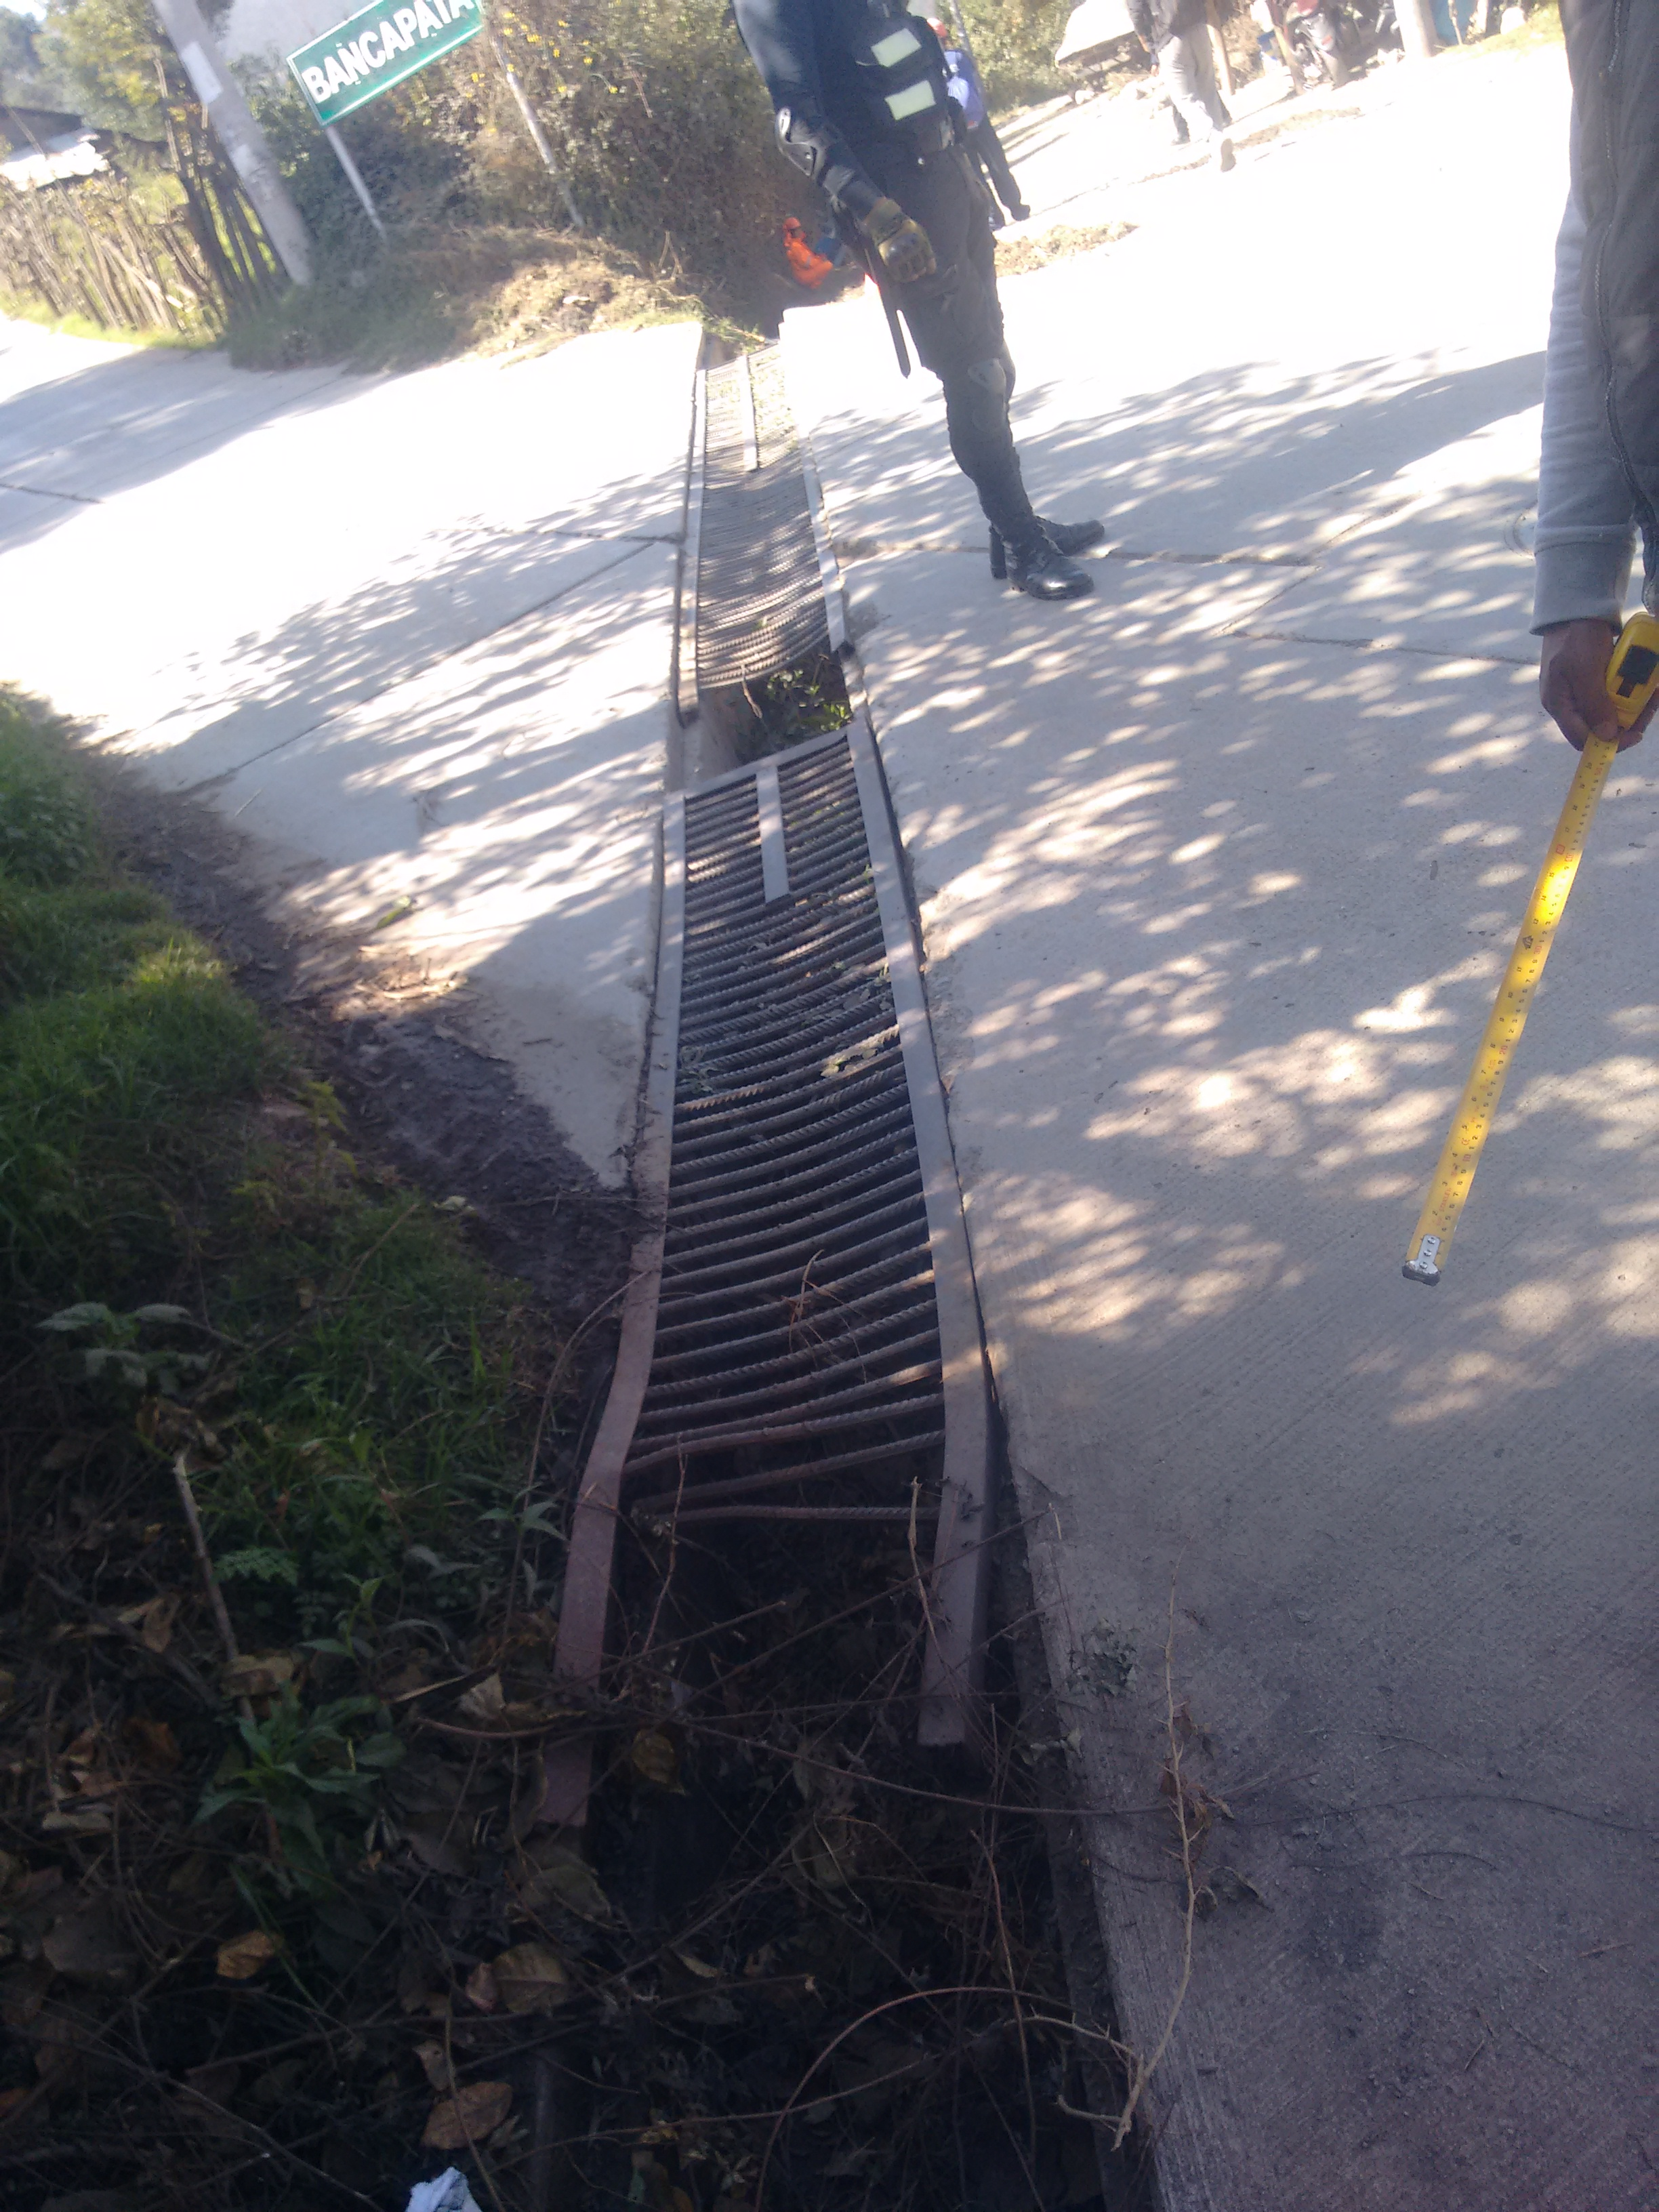
\includegraphics[height=0.8\linewidth]{3.21.jpg}
	\end{adjustbox}
	\caption[Trabajo de campo: Identificación de rejillas en mal estado]{Trabajo de campo , identificación de rejillas en mal estado en el sector de la carretera a Kerapata}
	\label{fig:img20230706125859989}
\end{figure}

\begin{figure}[h]
	\captionsetup{width=0.8\textwidth}
	\centering
	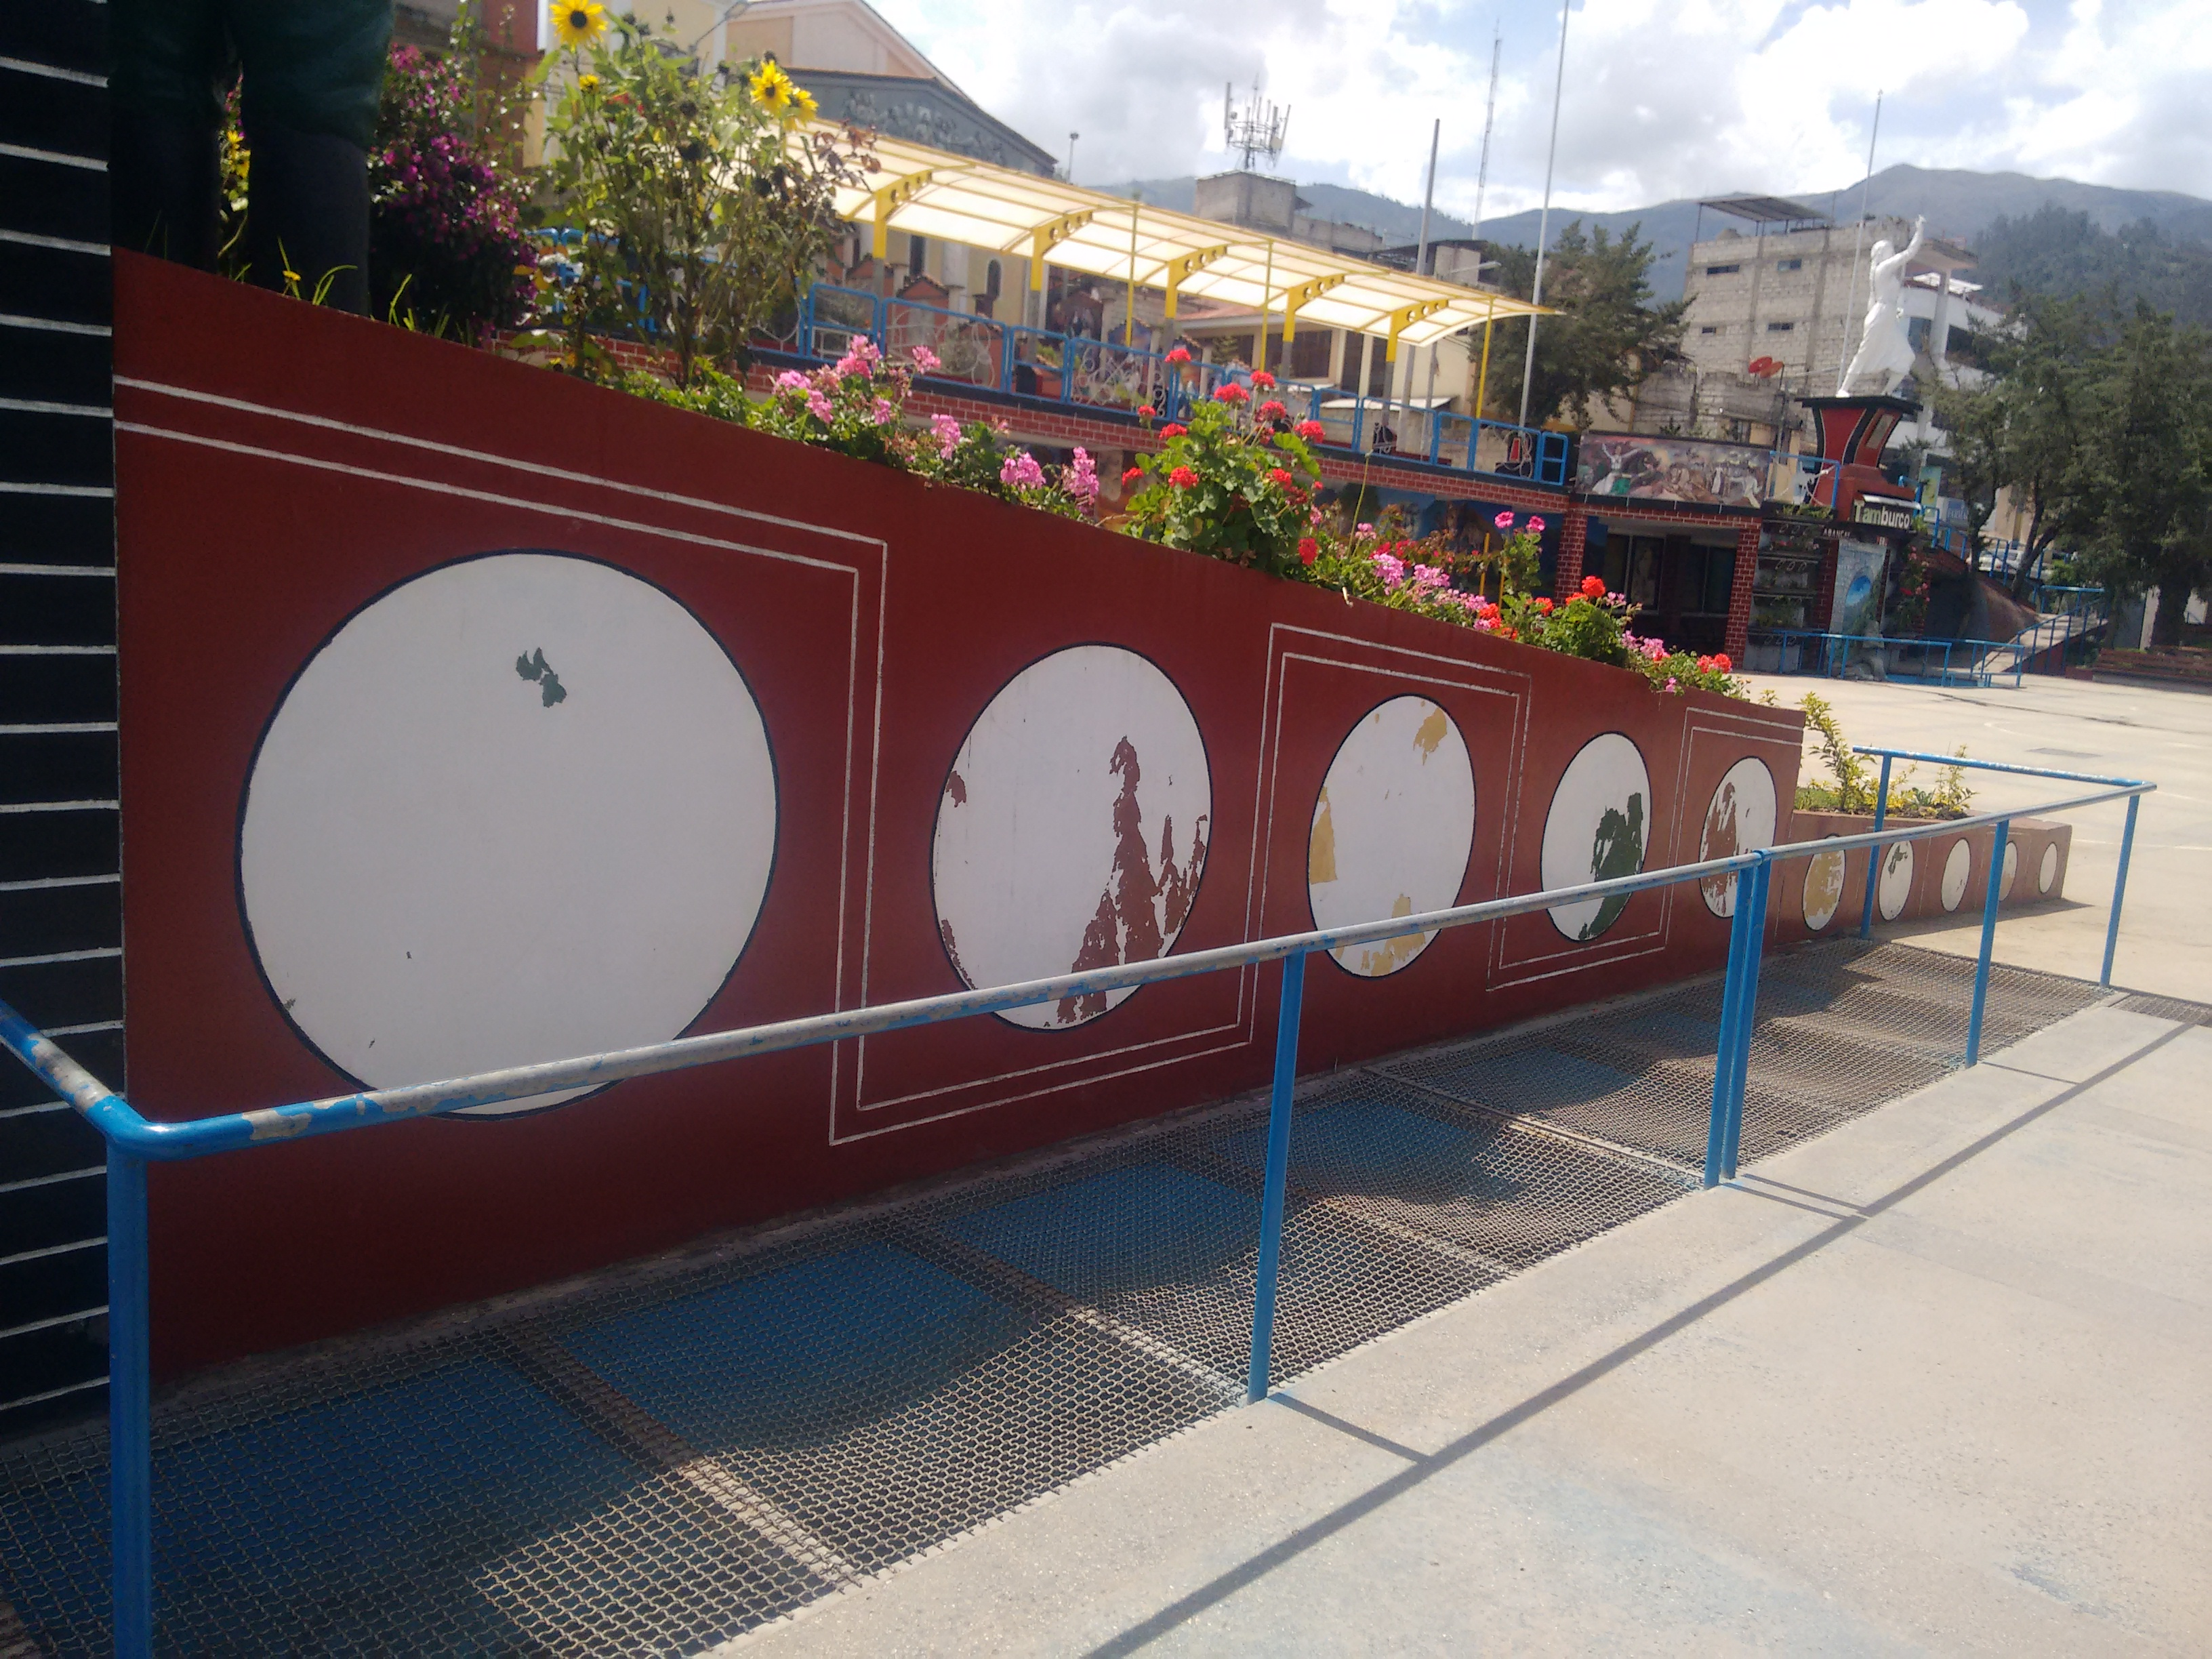
\includegraphics[width=0.8\linewidth]{3.22.jpg}
	\caption[Trabajo de campo: Cuantificación de daños y deterioro de la plaza de armas de Tamburco]{Trabajo de Campo, identificación de daños y deterioro de la plaza de armas de Tamburco}
	\label{fig:img20230414120419340}
\end{figure}

\begin{figure}[h]
	\captionsetup{width=0.8\textwidth}
	\centering
	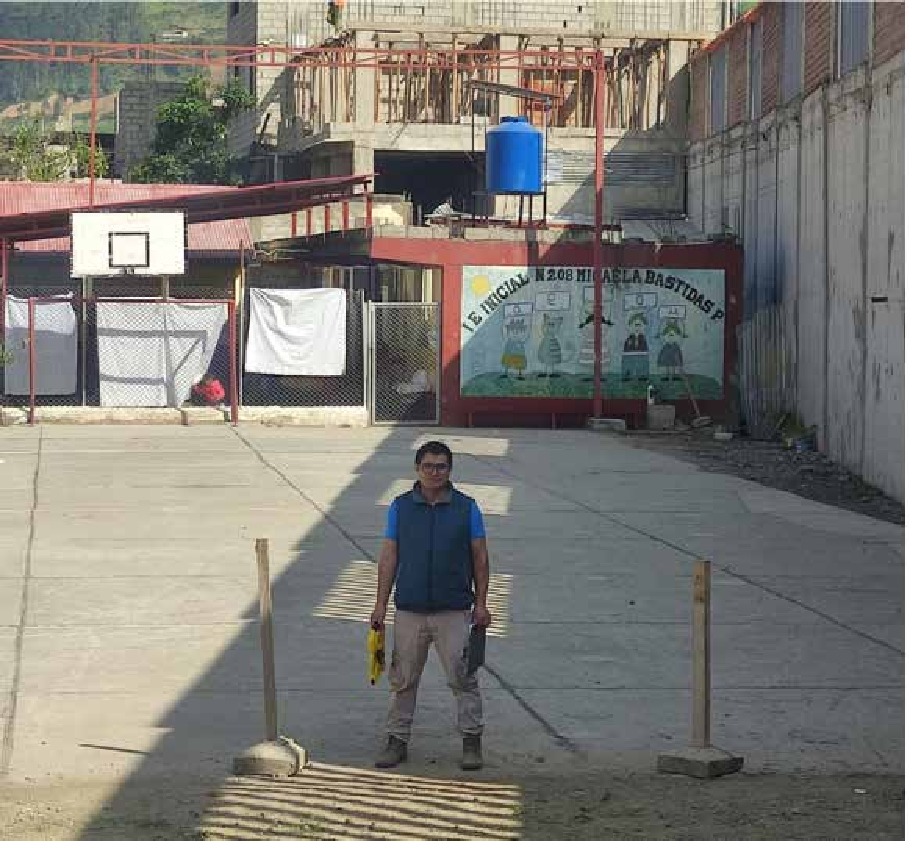
\includegraphics[width=0.8\linewidth]{3.16}
	\caption[Trabajo de Campo: Trazo y replanteo de las estructuras del colegio Micaela Bastidas]{Trazo y replanteo para el diseño de las estructuras en la plaza de honor del Colegio Micaela Bastidas.}
	\label{fig:asset-1}
\end{figure}

\begin{figure}[h]
	\captionsetup{width=0.8\linewidth}
	\centering
	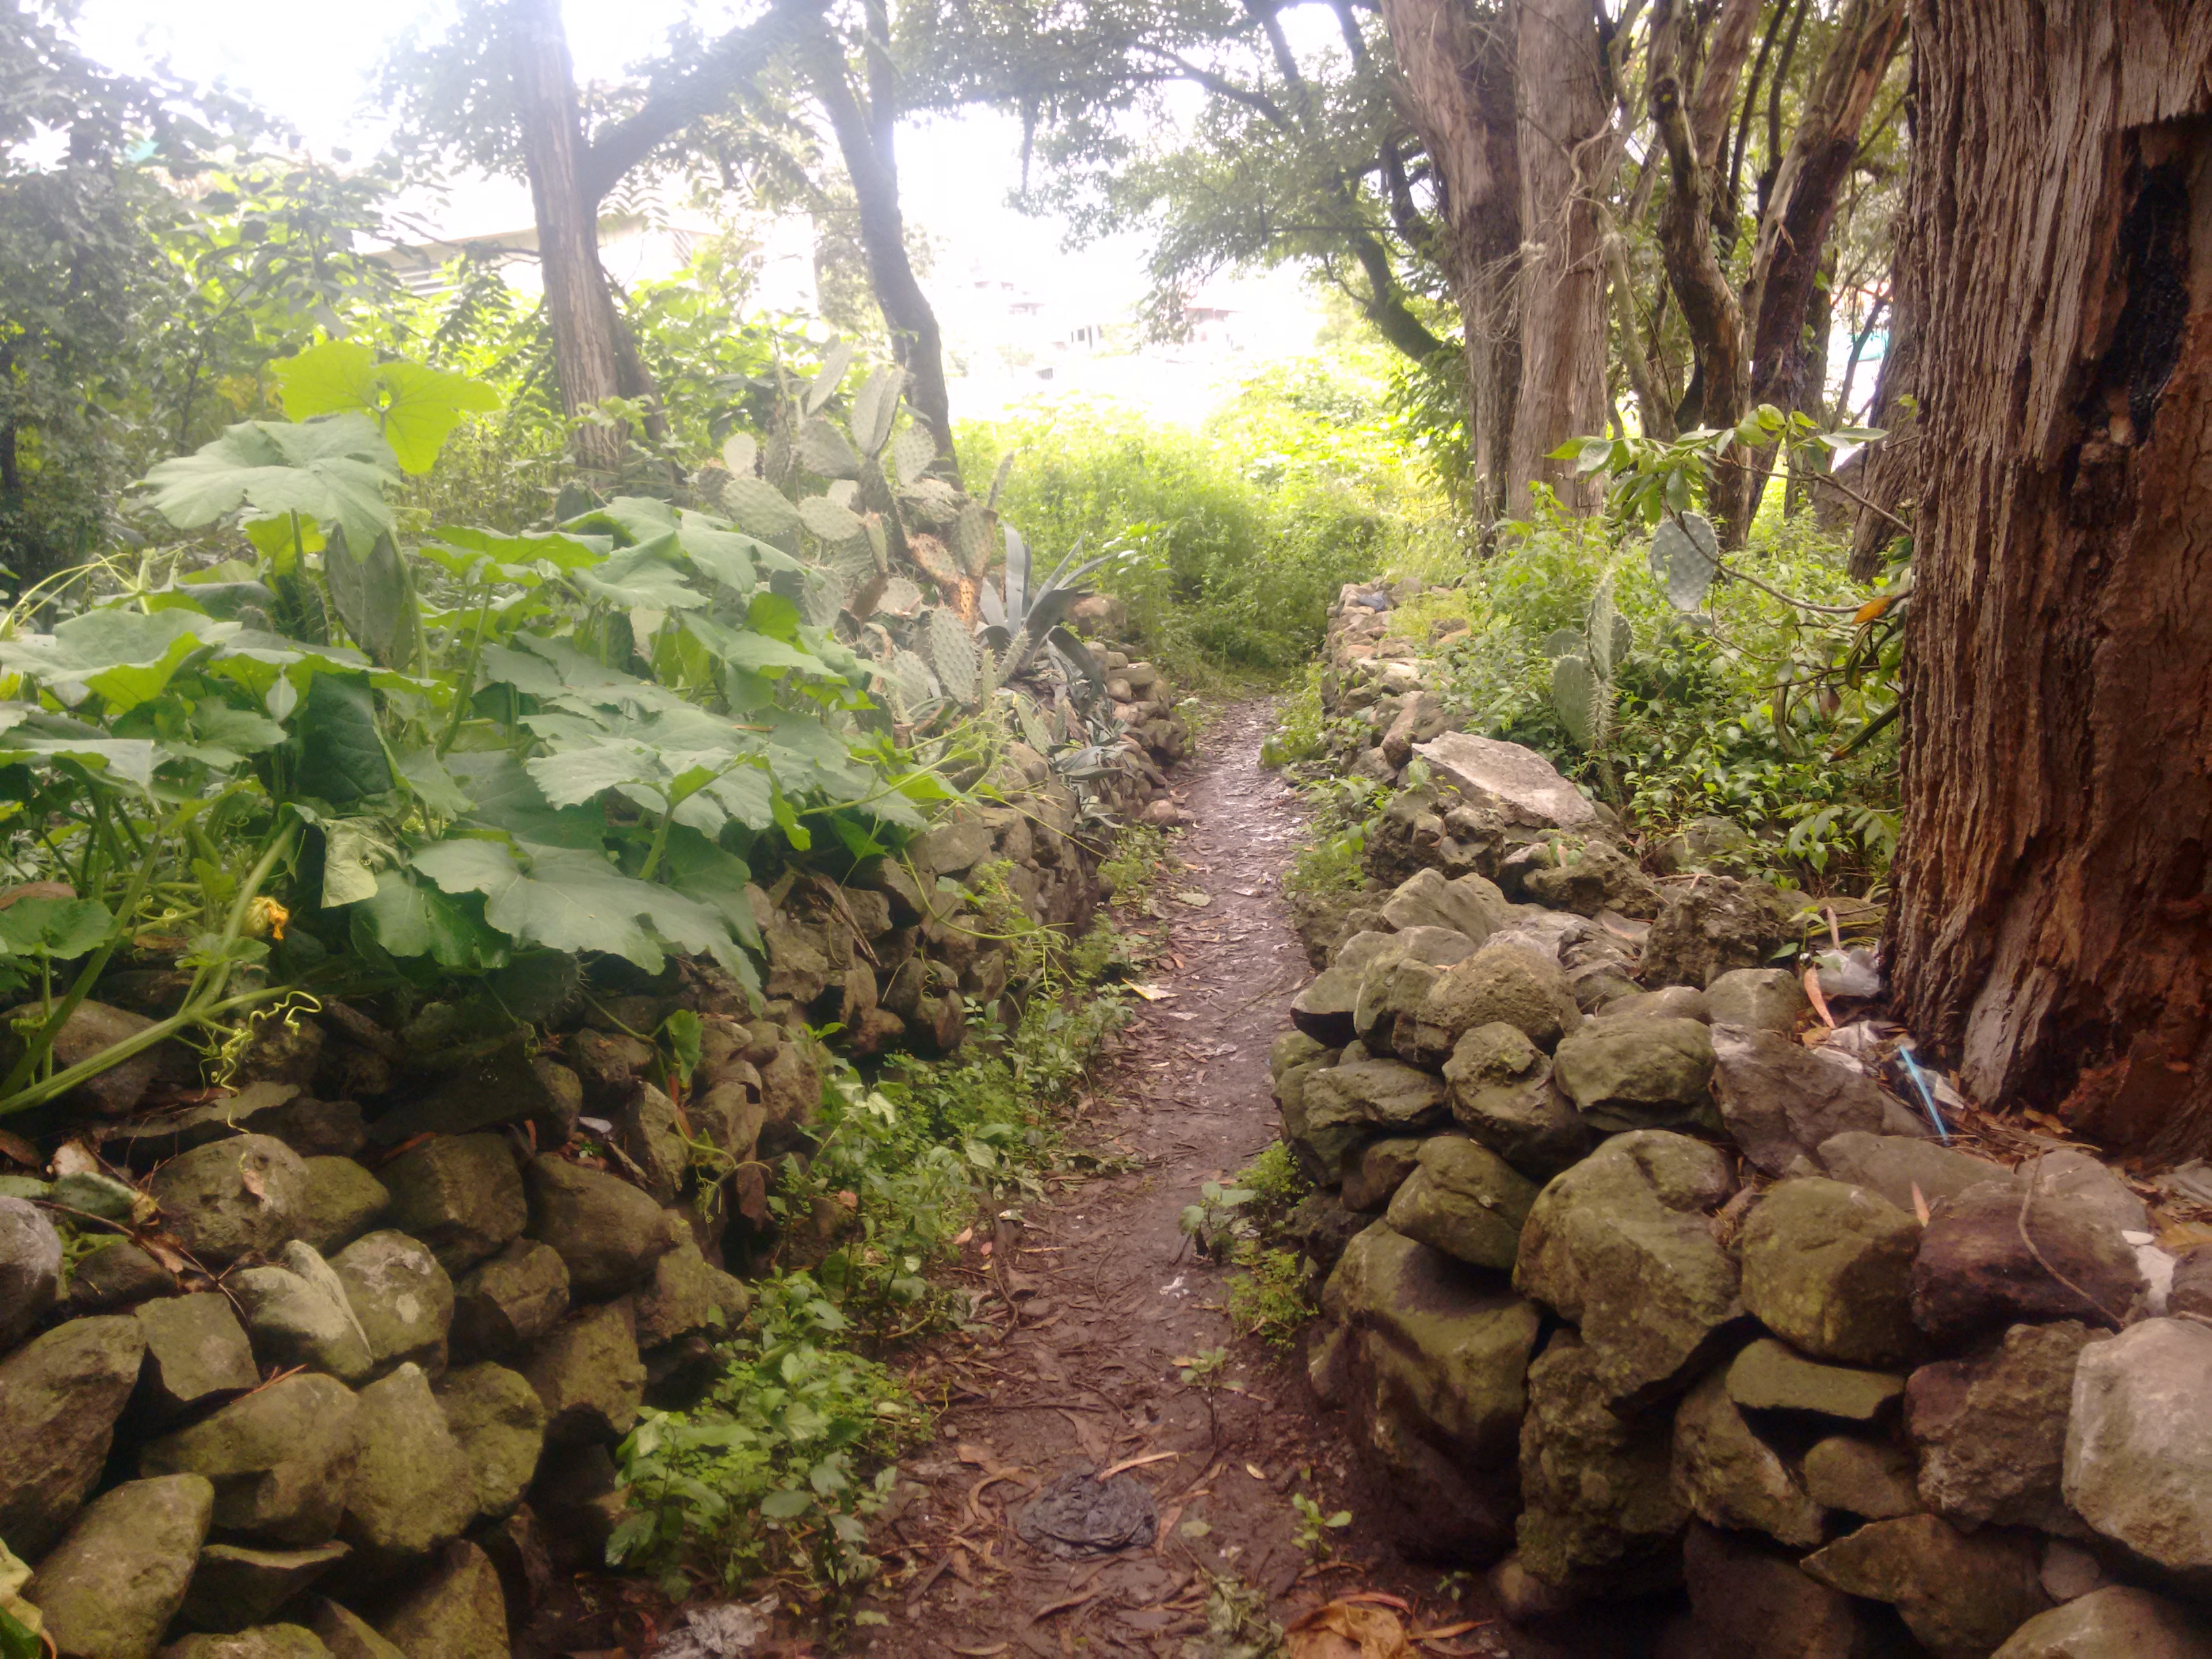
\includegraphics[width=0.8\linewidth]{3.14.jpg}
	\caption[Trabajo de campo: Apoyo en el levantamiento topográfico]{Apoyo en el levantamiento topográfico para el trazo de la alameda enla Av. Victor Acosta}
	\label{fig:img20230327093502248}
\end{figure}

%\pagestyle{fancy}
\chapter{APRECIACIÓN GENERAL}
Durante mi período como practicante, pude obtener percepciones valiosas en tres niveles distintos: en la entidad en sí, en la \acrshort{uep} (Unidad de Estudios y Proyectos), y, por último, en el entorno laboral en general. Estas experiencias me permitieron adquirir un entendimiento más completo y enriquecedor de la dinámica y funcionamiento de cada uno de estos ámbitos.
\section{Entidad}
\begin{enumerate}
	\item La entidad denominado \acrlong{mdt} está representado por Raúl Silva Campos como el alcalde del mismo, según la figura \ref{fig:organigrama-tamburco}, las decisiones económicas se toma en consejo municipal según la norma denominada Ley Orgánica de Municipalidades, aprobado por  \cite{CongresoRepublica2003}.
	\item Es evidente que en este entorno laboral, las decisiones presupuestarias se abordan con un enfoque responsable y cuidadoso. Al ser un proceso llevado a cabo en consejo, se busca asegurar la máxima responsabilidad en la toma de decisiones. Esta consideración colectiva demuestra una conciencia aguda de las posibles repercusiones a largo plazo y subraya el compromiso de asegurar la estabilidad financiera y el éxito sostenido en el futuro.
	\item Según el organigrama la autoridad responsable en el área de \acrshort{sgodur} (Sub-Gerencia de Obras y Desarrollo Urbano y Rural) es el ing. Ricardo H. Pinto Yupanqui, quien brindó la disponibilidad a atender las dudas y compartió sus conocimientos,  experiencias , consejos y recomendaciones cuando se requirieron.

	\item Existen restricciones, tales como el tope presupuestario que se disponen para solucionar un problema de infraestructura, no siendo suficiente con lo cual no se puede usar el recurso para resolver como debería ser.
\end{enumerate}
\section{Unidad de estudios y proyectos}
\begin{enumerate}
	\item La \acrlong{uep} oficina de la unidad de estudios y proyectos es la encargada de formular los proyectos, fichas de los mantenimientos, \acrshort{ioarr} ,siempre que esté en la capacidad logística y staff de profesionales capaces absolver los requerimientos que pueda surgir como consecuencia de los mismos, en este caso esta oficina dispone de una capacidad muy limitada ya que es una entidad es pequeña en cuanto a recursos.
	\item Los requerimientos para poder trabajar en estudios y proyectos en general son conocimientos en análisis estructural, concreto armado y demás cursos de pre-grado, así mismo también son necesarios el dominio de los diferentes software de ingeniería tales como:ETABS, SAFE, SAP 2000 y Robot Structural, no deja de ser de suma importancia el dominio de software de dibujo y modelado tales como: AutoCAD, Civil 3D, Revit.
	\item Definitivamente, un aspecto destacado que marca la diferencia en esta dinámica laboral son las habilidades blandas, en especial las habilidades interpersonales. Dado que surgen inevitablemente problemas y conflictos, es esencial contar con la capacidad de analizar y coordinar con las diversas partes involucradas, ya sean interesadas u opositoras, sin empeorar la situación. La habilidad para involucrar a todas las partes y hacerlas sentir parte de la solución es clave para gestionar eficazmente los desafíos y mantener un ambiente de trabajo productivo y armonioso.
	\item Es evidente que en esta oficina, cada proyecto requiere una perspectiva multidisciplinaria, ya que se depende de una variedad de especialidades para su ejecución. Esto subraya la importancia de contar con un equipo diversificado de expertos que puedan aportar sus conocimientos y habilidades únicas para abordar los desafíos de manera integral y efectiva. Esta sinergia entre diferentes disciplinas sin duda enriquece la calidad y el éxito de los proyectos que se emprenden en esta oficina.
	\item La lectura y comprensión de las normas internacionales, nacionales y manuales que rigen en nuestro país es una práctica fundamental en el ámbito laboral. Estas fuentes son invaluables al enfrentarse a situaciones ambiguas o cuestionamientos durante el trabajo, ya que proporcionan pautas claras y confiables para tomar decisiones informadas y asegurar el cumplimiento normativo. Por lo tanto, se vuelve imprescindible contar con un conocimiento actualizado de estas regulaciones para garantizar la legalidad y calidad en las acciones emprendidas.
\end{enumerate}

\section{Entorno laboral}
\begin{enumerate}
	\item Eh aqui donde se complican algunas cosas por diferentes causales tales como: Requisitos vagamente definidos, exigencias sin tener en cuenta los costos que implican, cambios a última hora, etc.
	\item En ocasiones sucede que el cliente opina basado en suposiciones y/o emociones, en estos casos es bueno explicarle al cliente de manera profesional.
	\item Sucede muy a menudo que los clientes solicitan modelos BIM a todos los profesionales y se niegan a aceptar trabajos realizados en software convencionales, en estos casos en necesario aclarar mediante directivas bien definidas antes de iniciar los trabajo y las implicancias de estos mismos.
	\item En lo que respecta a los demás aspectos, fue un ambiente con personas amables, colaborativos y cada uno con diferentes virtudes.
\end{enumerate}
%\pagestyle{fancy}
\chapter{CONCLUSIONES}
\begin{enumerate}
	\item La Municipalidad Distrital de Tamburco se ha enfocado en la ejecución de IOAAR \acrlong{ioarr} y mantenimientos. Esto se debe a las limitaciones de recursos, ya que la realización de estudios para proyectos de inversión pública (\acrshort{pip}) requeriría contar con oficinas más amplias y mantener un plantel de profesionales, lo cual implica asignar recursos adicionales. Esta estrategia permite optimizar los recursos disponibles y concentrarse en la ejecución de obras y acciones que beneficien directamente a la comunidad, aunque implique limitar la capacidad de realizar estudios detallados para nuevos proyectos de inversión pública.

	\item Es importante tener en cuenta que los practicantes que opten por realizar sus prácticas pre-profesionales en la Unidad de Estudios y Proyectos deben contar con conocimientos en diversos software de ingeniería. Estos incluyen herramientas como ETABS, SAFE y SAP2000, que son esenciales para el análisis y diseño de estructuras. Asimismo, se requiere experiencia en programas de dibujo asistido por computadora y modelado, como AutoCAD, Civil 3D y Revit, que son fundamentales para la elaboración de planos y modelos tridimensionales.
	Estos conocimientos permitirán a los practicantes contribuir de manera efectiva en la Unidad de Estudios y Proyectos, participando en la creación y desarrollo de proyectos de ingeniería de manera precisa y eficiente.

	\item Además de los conocimientos en software de ingeniería estructural y diseño, es igualmente importante que los practicantes tengan habilidades en áreas como Costos y Presupuestos, así como en Control y Seguimiento de Proyectos. En estas disciplinas, existen una amplia gama de software disponibles y el practicante puede elegir aquel con el que se sienta más cómodo o tenga experiencia previa. Esto asegura que puedan contribuir de manera efectiva en la planificación, gestión y control de los recursos y actividades relacionadas con los proyectos de ingeniería. La versatilidad en el manejo de diferentes herramientas es una habilidad valiosa para un profesional en el campo de la ingeniería.

	\item Es fundamental destacar que todos los criterios y decisiones tomadas en el proceso se basan rigurosamente en las normativas tanto nacionales como internacionales. Esto implica la lectura y comprensión detallada de reglamentos, manuales y demás documentos normativos pertinentes. Esta estricta adherencia a las regulaciones garantiza que los proyectos y procesos se desarrollen con los más altos estándares de calidad y seguridad, además de asegurar la legalidad y cumplimiento normativo en todas las etapas del trabajo.

	\item  Al concluir las prácticas pre-profesionales, el estudiante no solo adquiere conocimientos teóricos, sino también experiencias prácticas y aprendizajes invaluablemente enriquecedores al interactuar con profesionales experimentados en situaciones específicas y particulares. Cada caso y proyecto presenta desafíos y particularidades únicas, lo que permite al estudiante obtener una comprensión más profunda y aplicada de su futura profesión. Esta experiencia práctica es fundamental para su desarrollo profesional y le brinda una visión más completa y realista del campo en el que se desenvolverá.

	\item Al finalizar las prácticas pre-profesionales, el practicante no solo adquiere experiencia laboral, sino también establece relaciones laborales y amistades en el entorno profesional. Estas conexiones pueden jugar un papel crucial en el inicio de la carrera profesional, ya sea a través de recomendaciones para futuros trabajos remunerados o incluso mediante la posibilidad de ser contratado directamente por las personas con las que se trabajó durante las prácticas. El clima laboral positivo y las relaciones profesionales sólidas que se construyen durante esta etapa son activos valiosos que pueden abrir puertas importantes en el camino hacia una carrera exitosa.
\end{enumerate}
%\pagestyle{headings}
\chapter{RECOMENDACIONES}
	\begin{enumerate}
		
		\item Se recomienda a la entidad, establecer directrices claras y uniformes para la entrega y recepción de trabajos es fundamental para asegurar la calidad y consistencia en los proyectos realizados. Esto incluye especificar los componentes que deben estar incluidos en cada entrega, los formatos aceptables, los plazos y cualquier otra información relevante. Esta estandarización facilita el proceso de evaluación y asegura que todas las partes involucradas estén al tanto de lo que se espera en cada entrega. Así, se garantiza un proceso más eficiente y una mayor calidad en los trabajos realizados.
		
		\item Se recomienda a los practicantes contar con habilidades en el manejo de software especializado en ingeniería civil es esencial para contribuir de manera efectiva en proyectos y prácticas profesionales. Esto incluye herramientas como AutoCAD, Civil 3D, Revit, ETABS, SAFE, S10, MS Project, entre otros. Estos programas son fundamentales en la industria y permiten a los ingenieros realizar tareas de diseño, análisis y gestión de proyectos de manera eficiente. Quienes poseen habilidades en estas herramientas tienen un valor significativamente mayor en el campo laboral y están mejor preparados para aportar al desarrollo de proyectos de ingeniería civil.
		
		\item Para tomar decisiones efectivas en el entorno laboral, es crucial evitar depender exclusivamente de conocimientos empíricos, los cuales pueden ser inadecuados en muchas ocasiones. En su lugar, se recomienda recurrir a fuentes confiables como el jefe inmediato y otros expertos en el campo, buscando alinear las decisiones con las normativas vigentes. Esta consulta proporciona valiosos insights y perspectivas diversas, permitiendo llegar a soluciones más sólidas. Asimismo, es esencial mantenerse al tanto de las regulaciones actuales para garantizar la legalidad, seguridad y calidad en las acciones emprendidas.
		\item Durante mi experiencia como practicante, pude constatar un factor crucial en el ámbito de la remodelación y mantenimiento de espacios: la falta de consideración de las especialidades de comunicaciones, como el cableado de televisión e internet, ha sido una fuente recurrente de problemas. En el contexto actual, donde los servicios de internet, intercomunicadores y televisión son cada vez más relevantes en nuestra vida cotidiana, es imperativo reconocer la necesidad de integrar adecuadamente estas tecnologías en los proyectos de construcción y renovación.
		
	\end{enumerate}
%%%%%%%%%%%%%%%%%%%%%%%%%%%%%%%%%%%%%%%%%%%%%%%%%%%%%%%%%%%%%%%%%%%%%%%%%%%%%%
\backmatter
\appendix
\chapter{Apéndice A:Planos}
\begin{figure}[H]
	\centering
	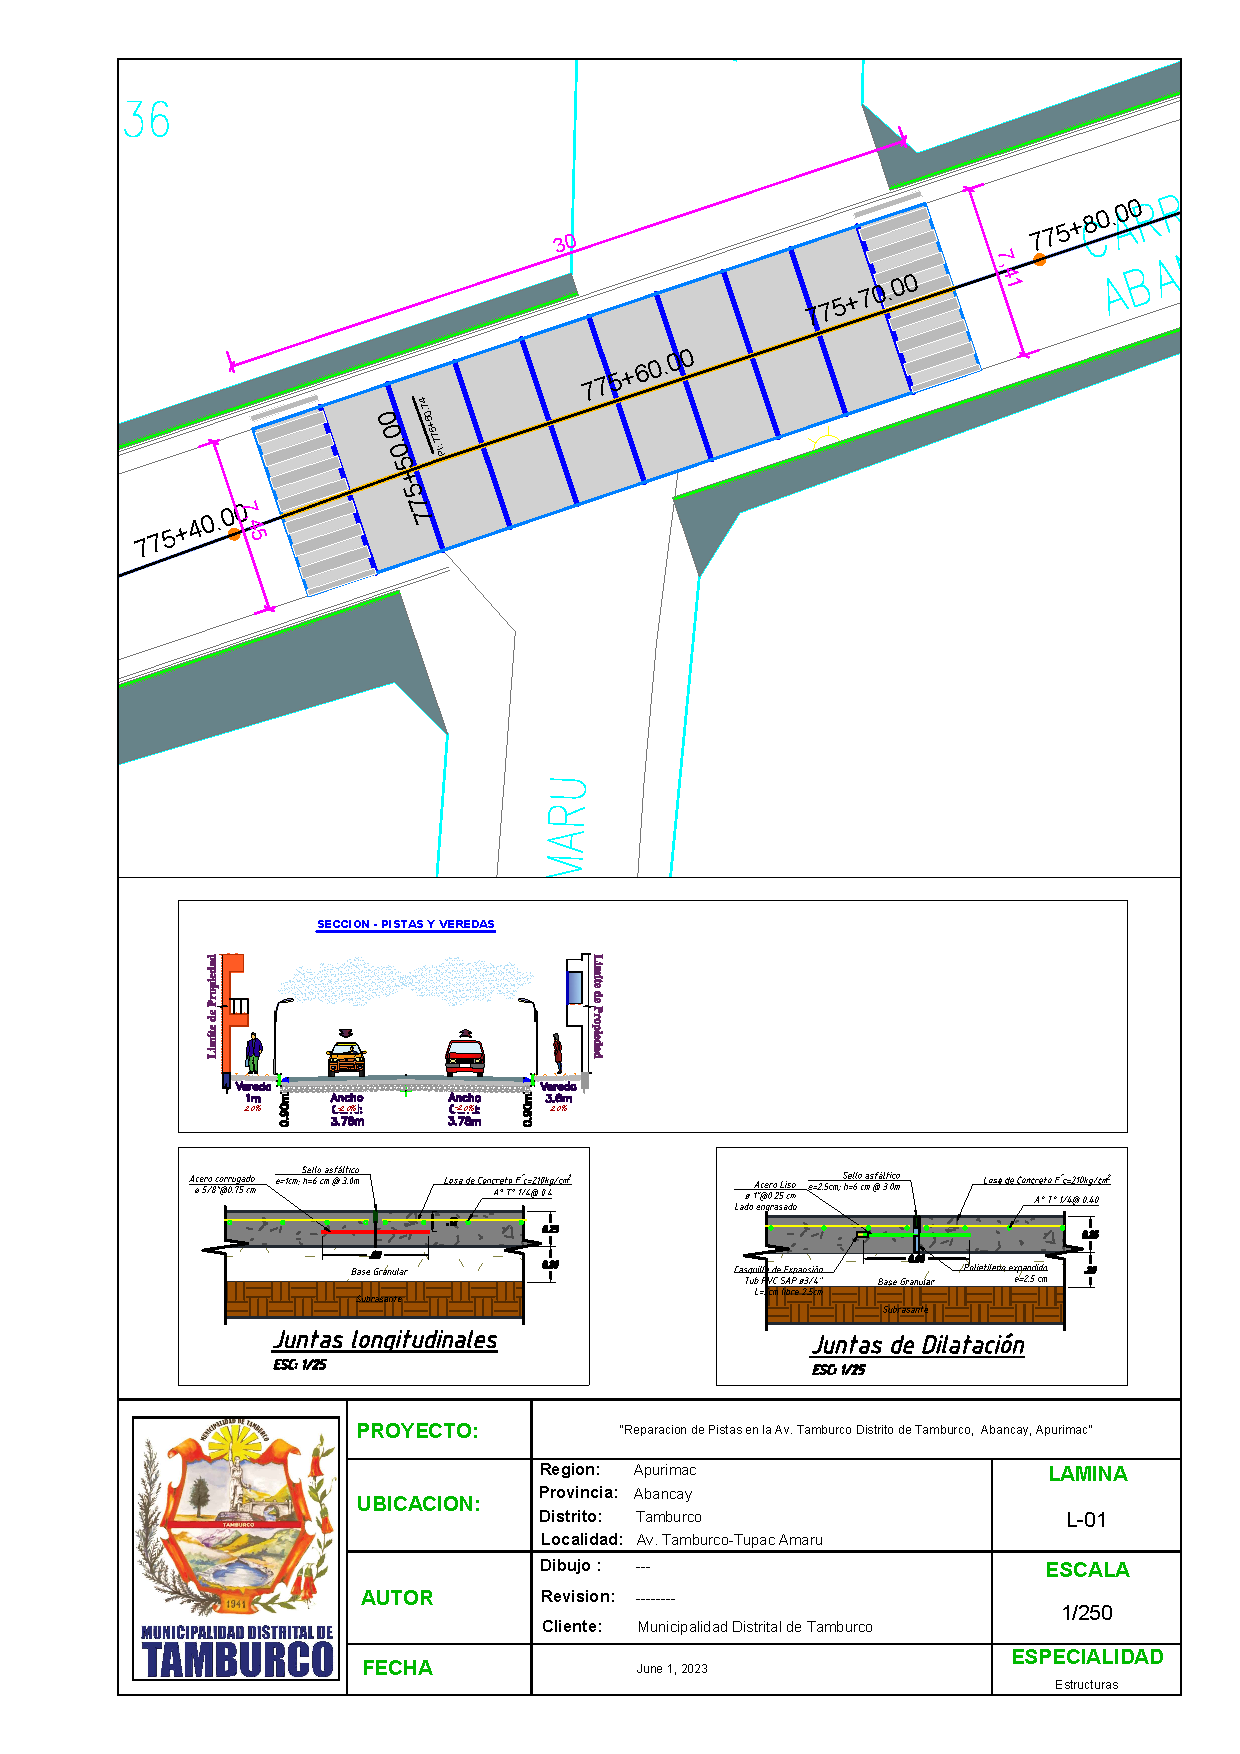
\includegraphics[height=23cm]{7.2.pdf}
	\caption{Plano del área de intervención en la Av. Tamburco-Tupac Amaru}
	\label{fig:7.2}
\end{figure}
\newpage
\begin{landscape}
	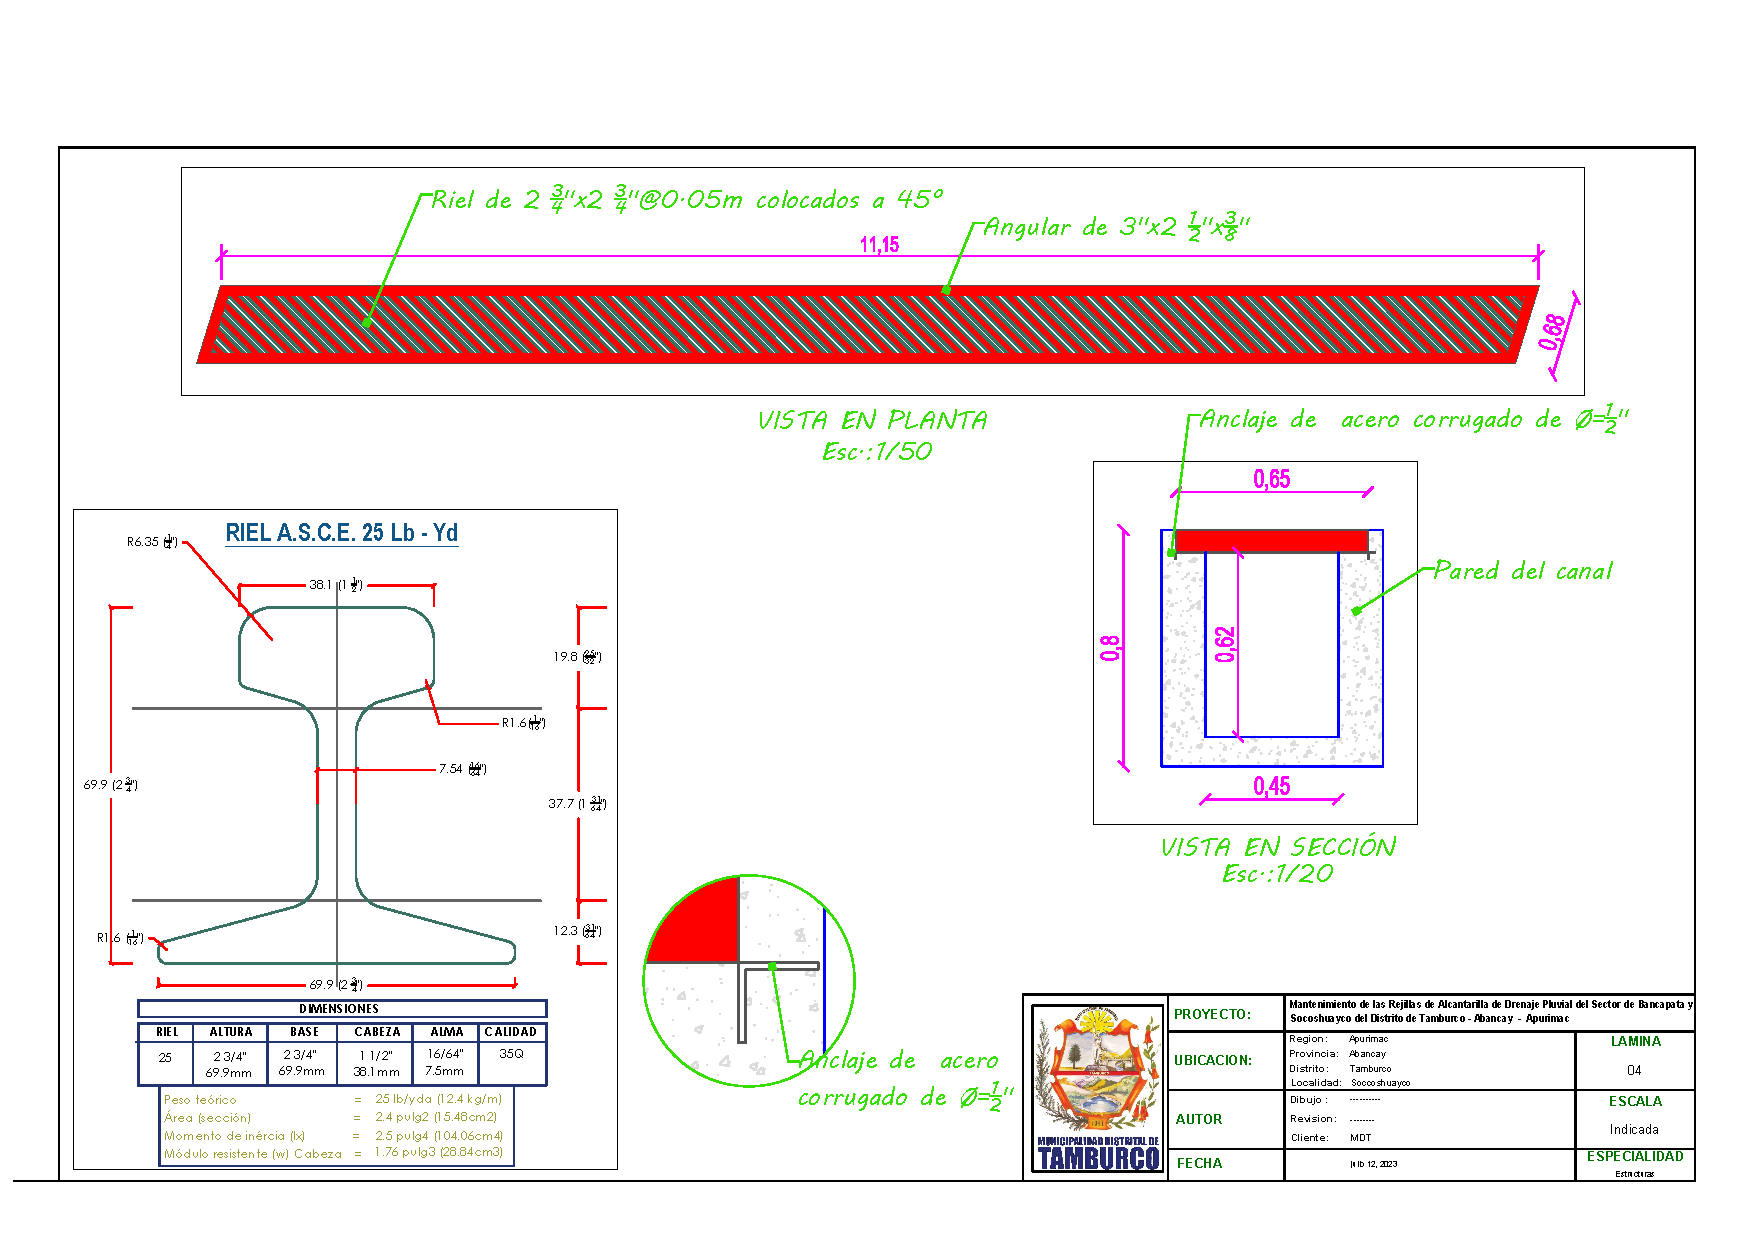
\includepdf[pages=-, angle=90]{7.3}
\end{landscape}


\newgeometry{margin=0.7in,landscape} 
    \begin{landscape}
        \chapter{Apéndice B:Mapas}
    \begin{figure}[htb]
        \centering
        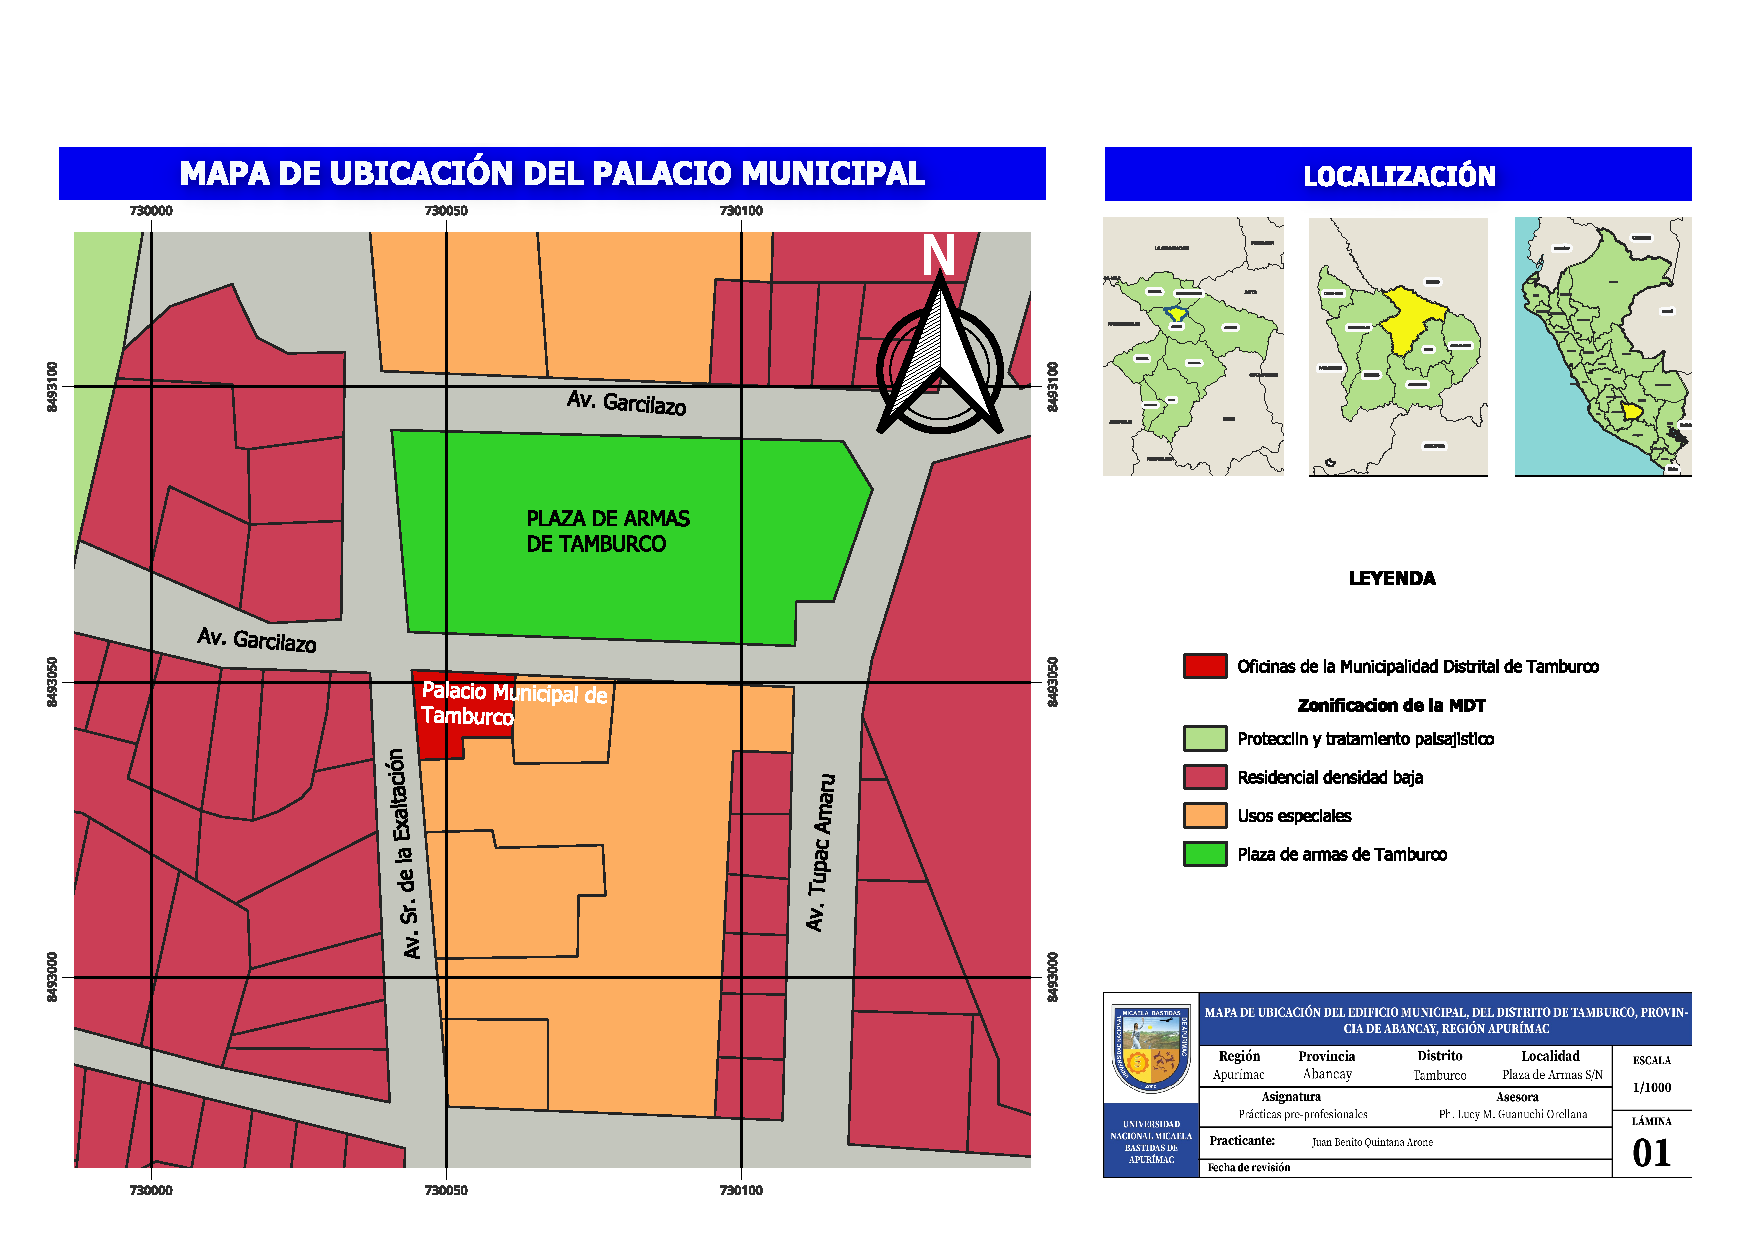
\includegraphics[scale=0.7]{7.1}
        \caption{Mapa de ubicación del Palacio Municipal}
        \label{fig:7.1}
    \end{figure}
    \end{landscape}   
\restoregeometry % Restaura la geometría original

\printbibliography[title=BIBLIOGRAFÍA]

\end{document}